
\documentclass[sigconf,balance=false]{acmart}
\usepackage{popets} 
\usepackage{tikz}
\usepackage{amsmath}
\usepackage{lipsum}% http://ctan.org/pkg/lipsum
\usepackage{multicol}% http://ctan.org/pkg/multicols
\usepackage{graphicx}% http://ctan.org/pkg/graphicx
\usepackage{listings,multicol}
\usepackage{color}
\usepackage{array}
\usepackage{booktabs}
\usepackage[tableposition=below]{caption}\captionsetup[table]{skip=10pt}
\usepackage{multirow}
\usepackage{colortbl}
\newcommand{\ltgrey}{\rowcolor[gray]{0.88}} %DIF > 

\definecolor{dkgreen}{rgb}{0,0.6,0}
\definecolor{gray}{rgb}{0.5,0.5,0.5}
\definecolor{mauve}{rgb}{0.58,0,0.82}

\setcopyright{popets} %DIF > 
\copyrightyear{YYYY} %DIF > 
% Issue info %DIF > 
\acmYear{YYYY} %DIF > 
\acmVolume{YYYY} %DIF > 
\acmNumber{X} %DIF > 
\acmDOI{XXXXXXX.XXXXXXX} %DIF > 
\acmISBN{} %DIF > 
\acmConference{Proceedings on Privacy Enhancing Technologies} %DIF > 
\settopmatter{printacmref=false,printccs=false,printfolios=true} %DIF > 
\def\checkmark{{\footnotesize $\bigstar$}}

\lstset{
frame=tb,
language=Java,
stringstyle=\color{mauve},
breaklines=true,
commentstyle=\color{dkgreen},
columns=fullyflexible,
keywordstyle=\color{blue},
aboveskip=0.1mm,
belowskip=0.1mm,
linewidth=\columnwidth
}

% inlined bib file
\usepackage{filecontents}

\definecolor{chicagomaroon}{rgb}{0.5, 0.0, 0.0}

\iffalse
\newcommand{\alex}[1]{\textcolor{chicagomaroon}{\noindent[AL: #1]}}
\newcommand{\sumanth}[1]{\textcolor{violet}{\noindent[SR: #1]}}
\newcommand{\damon}[1]{\textcolor{blue}{\noindent[DM: #1]}}
\newcommand{\sam}[1]{\textcolor{orange}{\noindent[SH: #1]}}
\newcommand{\todo}[1]{\textsf{\textcolor{red}{[TODO: #1]}}}
\newcommand{\grant}[1]{\textsf{\textcolor{teal}{[GH: #1]}}}
\newcommand{\geoff}[1]{\textcolor{purple}{\noindent[GV: #1]}}
\newcommand{\stefan}[1]{\textcolor{green}{\noindent[SS: #1]}}
\iffalse

\fi

\else
\newcommand{\alex}[1]{}
\newcommand{\sumanth}[1]{}
\newcommand{\todo}[1]{}
\newcommand{\grant}[1]{}
\newcommand{\geoff}[1]{}
\newcommand{\stefan}[1]{}
\newcommand{\damon}[1]{}
\newcommand{\sam}[1]{}

\fi

\newcommand{\rating}[1]{%
	\begin{tikzpicture}[x=1ex,y=1ex]
		\begin{scope}
			\clip (0,1) circle (1);
			\fill[lightgray] (-1,0) rectangle (1,#1/50);
		\end{scope}
		\draw[black, thin, radius=1] (0,1) circle;
	\end{tikzpicture}%
}

%-------------------------------------------------------------------------------
%DIF PREAMBLE EXTENSION ADDED BY LATEXDIFF
%DIF UNDERLINE PREAMBLE %DIF PREAMBLE
\RequirePackage[normalem]{ulem} %DIF PREAMBLE
\RequirePackage{color}\definecolor{RED}{rgb}{1,0,0}\definecolor{BLUE}{rgb}{0,0,1} %DIF PREAMBLE
\providecommand{\DIFadd}[1]{{\protect\color{blue}\uwave{#1}}} %DIF PREAMBLE
\providecommand{\DIFdel}[1]{{\protect\color{red}\sout{#1}}}                      %DIF PREAMBLE
%DIF SAFE PREAMBLE %DIF PREAMBLE
\providecommand{\DIFaddbegin}{} %DIF PREAMBLE
\providecommand{\DIFaddend}{} %DIF PREAMBLE
\providecommand{\DIFdelbegin}{} %DIF PREAMBLE
\providecommand{\DIFdelend}{} %DIF PREAMBLE
%DIF FLOATSAFE PREAMBLE %DIF PREAMBLE
\providecommand{\DIFaddFL}[1]{\DIFadd{#1}} %DIF PREAMBLE
\providecommand{\DIFdelFL}[1]{\DIFdel{#1}} %DIF PREAMBLE
\providecommand{\DIFaddbeginFL}{} %DIF PREAMBLE
\providecommand{\DIFaddendFL}{} %DIF PREAMBLE
\providecommand{\DIFdelbeginFL}{} %DIF PREAMBLE
\providecommand{\DIFdelendFL}{} %DIF PREAMBLE
\newcommand{\DIFscaledelfig}{0.5}
%DIF HIGHLIGHTGRAPHICS PREAMBLE %DIF PREAMBLE
\RequirePackage{settobox} %DIF PREAMBLE
\RequirePackage{letltxmacro} %DIF PREAMBLE
\newsavebox{\DIFdelgraphicsbox} %DIF PREAMBLE
\newlength{\DIFdelgraphicswidth} %DIF PREAMBLE
\newlength{\DIFdelgraphicsheight} %DIF PREAMBLE
% store original definition of \includegraphics %DIF PREAMBLE
\LetLtxMacro{\DIFOincludegraphics}{\includegraphics} %DIF PREAMBLE
\newcommand{\DIFaddincludegraphics}[2][]{{\color{blue}\fbox{\DIFOincludegraphics[#1]{#2}}}} %DIF PREAMBLE
\newcommand{\DIFdelincludegraphics}[2][]{% %DIF PREAMBLE
\sbox{\DIFdelgraphicsbox}{\DIFOincludegraphics[#1]{#2}}% %DIF PREAMBLE
\settoboxwidth{\DIFdelgraphicswidth}{\DIFdelgraphicsbox} %DIF PREAMBLE
\settoboxtotalheight{\DIFdelgraphicsheight}{\DIFdelgraphicsbox} %DIF PREAMBLE
\scalebox{\DIFscaledelfig}{% %DIF PREAMBLE
\parbox[b]{\DIFdelgraphicswidth}{\usebox{\DIFdelgraphicsbox}\\[-\baselineskip] \rule{\DIFdelgraphicswidth}{0em}}\llap{\resizebox{\DIFdelgraphicswidth}{\DIFdelgraphicsheight}{% %DIF PREAMBLE
\setlength{\unitlength}{\DIFdelgraphicswidth}% %DIF PREAMBLE
\begin{picture}(1,1)% %DIF PREAMBLE
\thicklines\linethickness{2pt} %DIF PREAMBLE
{\color[rgb]{1,0,0}\put(0,0){\framebox(1,1){}}}% %DIF PREAMBLE
{\color[rgb]{1,0,0}\put(0,0){\line( 1,1){1}}}% %DIF PREAMBLE
{\color[rgb]{1,0,0}\put(0,1){\line(1,-1){1}}}% %DIF PREAMBLE
\end{picture}% %DIF PREAMBLE
}\hspace*{3pt}}} %DIF PREAMBLE
} %DIF PREAMBLE
\LetLtxMacro{\DIFOaddbegin}{\DIFaddbegin} %DIF PREAMBLE
\LetLtxMacro{\DIFOaddend}{\DIFaddend} %DIF PREAMBLE
\LetLtxMacro{\DIFOdelbegin}{\DIFdelbegin} %DIF PREAMBLE
\LetLtxMacro{\DIFOdelend}{\DIFdelend} %DIF PREAMBLE
\DeclareRobustCommand{\DIFaddbegin}{\DIFOaddbegin \let\includegraphics\DIFaddincludegraphics} %DIF PREAMBLE
\DeclareRobustCommand{\DIFaddend}{\DIFOaddend \let\includegraphics\DIFOincludegraphics} %DIF PREAMBLE
\DeclareRobustCommand{\DIFdelbegin}{\DIFOdelbegin \let\includegraphics\DIFdelincludegraphics} %DIF PREAMBLE
\DeclareRobustCommand{\DIFdelend}{\DIFOaddend \let\includegraphics\DIFOincludegraphics} %DIF PREAMBLE
\LetLtxMacro{\DIFOaddbeginFL}{\DIFaddbeginFL} %DIF PREAMBLE
\LetLtxMacro{\DIFOaddendFL}{\DIFaddendFL} %DIF PREAMBLE
\LetLtxMacro{\DIFOdelbeginFL}{\DIFdelbeginFL} %DIF PREAMBLE
\LetLtxMacro{\DIFOdelendFL}{\DIFdelendFL} %DIF PREAMBLE
\DeclareRobustCommand{\DIFaddbeginFL}{\DIFOaddbeginFL \let\includegraphics\DIFaddincludegraphics} %DIF PREAMBLE
\DeclareRobustCommand{\DIFaddendFL}{\DIFOaddendFL \let\includegraphics\DIFOincludegraphics} %DIF PREAMBLE
\DeclareRobustCommand{\DIFdelbeginFL}{\DIFOdelbeginFL \let\includegraphics\DIFdelincludegraphics} %DIF PREAMBLE
\DeclareRobustCommand{\DIFdelendFL}{\DIFOaddendFL \let\includegraphics\DIFOincludegraphics} %DIF PREAMBLE
%DIF END PREAMBLE EXTENSION ADDED BY LATEXDIFF


\begin{document}
%-------------------------------------------------------------------------------

%don't want date printed
\date{}

% make title bold and 14 pt font (Latex default is non-bold, 16 pt)
\title{No Privacy Among Spies: Assessing the Functionality and Insecurity of Consumer Android Spyware Apps}
%for single author (just remove % characters)
% \author{
%DIF <  {\rm Your N.\ Here}\\
%DIF <  Your Institution
%DIF >  {\rm Enze Liu}\\
%DIF >  Meta
% \and
%DIF <  {\rm Second Name}\\
%DIF <  Second Institution
%DIF >  {\rm Sumanth Rao}\\
% % copy the following lines to add more authors
% % \and
% % {\rm Name}\\
% %Name Institution
% } % end author
%DIF >  \affiliation{UC San Diegp}

\DIFaddbegin \author{\DIFadd{Enze Liu}}
\orcid{0000-0003-4288-8485}
\affiliation{
	\institution{UC San Diego}
	\city{La Jolla}
	\state{CA}
	\country{USA}
}
%DIF > \affiliation{...}
\email{e7liu@eng.ucsd.edu}
\author{\DIFadd{Sumanth Rao}}
\affiliation{
	\institution{UC San Diego}
	\city{La Jolla}
	\state{CA}
	\country{USA}
}
\email{svrao@ucsd.edu}
\author{\DIFadd{Sam Havron}}
\affiliation{
	\institution{Cornell Tech}
	\city{New York}
	\state{NY}
	\country{USA}
}
\email{havron@cs.cornell.edu}
\author{\DIFadd{Grant Ho}}
\affiliation{
	\institution{UC San Diego}
	\city{La Jolla}
	\state{CA}
	\country{USA}
}
\email{grho@eng.ucsd.edu}
\author{\DIFadd{Stefan Savage}}
\affiliation{
	\institution{UC San Diego}
	\city{La Jolla}
	\state{CA}
	\country{USA}
}
\email{savage@cs.ucsd.edu}
\author{\DIFadd{Geoffrey M. Voelker}}
\affiliation{
	\institution{UC San Diego}
	\city{La Jolla}
	\state{CA}
	\country{USA}
}
\email{voelker@cs.ucsd.edu}
\author{\DIFadd{Damon McCoy}}
\affiliation{
	\institution{New York University}
	\city{New York}
	\state{NY}
	\country{USA}
}
\email{mccoy@nyu.edu}
%DIF > \affiliation{...}
%DIF > \affiliation{...}

%DIF >  \and
%DIF >  {\rm Sam Havron}\\
%DIF >  Meta
%DIF >  {\rm Grant Ho}\\
%DIF >  UC San Diego
%DIF >  {\rm Stefan Savage}\\
%DIF >  UC San Diego
%DIF >  {\rm Geoffrey M. Voelker}\\
%DIF >  UC San Diego
%DIF >  {\rm Damon McCoy}\\
%DIF >  New York University

\DIFaddend \begin{abstract}
{ Consumer mobile spyware apps covertly monitor a user's activities
  (i.e., text messages, phone calls, e-mail, location, etc.) and
  transmit that information over the Internet to support remote
  surveillance.  Unlike conceptually similar apps used for state
  espionage, so-called ``stalkerware'' apps are mass-marketed to
  consumers on a retail basis and expose a far broader range of
  victims to invasive monitoring.  Today the market for such apps is
  large enough to support dozens of competitors\DIFaddbegin \DIFadd{, }\DIFaddend with individual
  vendors reportedly monitoring \DIFdelbegin \DIFdel{over 400,000 }\DIFdelend \DIFaddbegin \DIFadd{hundreds of thousands of }\DIFaddend phones.
  However, while the research community is well aware of the existence
  of such apps, \DIFdelbegin \DIFdel{there had not been a large-scale technical analysis of these apps using a consistent methodology.
This has left us with an ad-hoc }\DIFdelend \DIFaddbegin \DIFadd{our }\DIFaddend understanding of the mechanisms \DIFdelbegin \DIFdel{by which they operate.
}%DIFDELCMD < 

%DIFDELCMD < %%%
\DIFdelend \DIFaddbegin \DIFadd{they use to
  operate remains ad hoc.  }\DIFaddend In this work, we perform an in-depth
  technical analysis of \DIFdelbegin \DIFdel{the fourteen leading families of }\DIFdelend \DIFaddbegin \DIFadd{fourteen distinct leading }\DIFaddend mobile spyware apps
  targeting Android phones. We document the range of mechanisms used
  to monitor user activity of various kinds (e.g., photos, text
  messages, live microphone access) --- primarily through the creative
  abuse of Android APIs. We also discover previously undocumented
  methods these apps use to hide from detection and to achieve
  persistence\DIFdelbegin \DIFdel{(one of which Android considers outside their threat model and declined to fix). As well}\DIFdelend \DIFaddbegin \DIFadd{. Additionally}\DIFaddend , we document the measures taken by each
  app to protect the privacy of the sensitive data they collect,
  identifying a range of failings on the part of spyware vendors
  (including privacy-sensitive data sent in the clear or stored in the
  cloud with little or no protection).  }


%  Consumer mobile spyware apps have gained much popularity over the years as they
%dramatically lower the entry barrier for ordinary people to surveil others. The
%widespread \sam{use or availability?} of these apps also raises great concerns
%due to their privacy-invasive nature (that they covertly collect sensitive user
%data) and poor security hygiene (that they do not protect users' data well).
%Thus far, the security community has a good understanding of what features
%spyware apps offer, but lacks the knowledge of how they achieve those features
%technically.  Similarly, while reportedly spyware apps have weak security posture
%(e.g., some of them transfer data in plaintext), there exists only
%cursory investigation of existing security and privacy vulnerabilities.
%
%In this work, we perform the first in-depth technical analysis of how spyware
%apps achieve various features by using existing APIs in unexpected and
%sophisticated ways, discovering a few novel venues of abusing Android APIs. Our
%work not only sheds light on the technical capabilities of spyware apps but also
%helps the community better appreciate the underlying technical problems and
%gaps in existing Android privacy safeguards.
%We also discuss potential solutions to mitigate the issues identified.
%We also conduct a security assessment of both the client-side and the server-side
%of consumer spyware apps. We document, ironically, how little effort they have
%made to protect the collected user data that is often sensitive.

\end{abstract}


\maketitle

%-------------------------------------------------------------------------------
\section{Introduction}
%-------------------------------------------------------------------------------

Consumer mobile spyware --- software that covertly gathers information
on a mobile device and transfers that information to a remote server
--- has existed for at least two decades, but has grown significantly
in popularity in recent years.  In one recent study from Norton Labs
~\cite{AYearAft87:online}, the number of devices identified with
spyware apps increased by 63\% between September 2020 and May 2021. A
similar report from Avast saw a 93\% increase in the use of spyware
apps in the UK over a similar period~\cite{UseofSta91:online}.

Sold under a wide variety of brand names --- TheTruthSpy, mSpy,
Flexispy and so on --- these apps are marketed directly to the general
public.  They are relatively cheap (typically between \$30 and \$100
per month), easy to install and do not require specialized technical
know-how to deploy or operate.  Indeed, the only requirement for such
software is \DIFdelbegin \DIFdel{temporary }\DIFdelend \DIFaddbegin \emph{\DIFadd{temporary}} \DIFaddend physical access to the target device.  After
installation, the owner of the target device may have no knowledge
that anything has changed.  But the intimate details of their life can
now be sent to another party, including the contents of their text
messages, email messages, photos taken and received, and even live
recording from their microphone and camera.  Unsurprisingly, such
``stalkerware'' has been implicated in a range of abuses including
intimate partner violence~\cite{chatterjee2018spyware} and
cyberstalking~\cite{woodlock2017abuse}.

Moreover, \DIFdelbegin \DIFdel{the exposure of sensitive }\DIFdelend \DIFaddbegin \DIFadd{privacy failures in the ``back end'' software used to store and
display exfiltrated data means that exposure of the victims' private }\DIFaddend information is not \DIFdelbegin \DIFdel{necessarily
limited to }\DIFdelend \DIFaddbegin \DIFadd{limited to just the abuser who installs }\DIFaddend the \DIFdelbegin \DIFdel{party who installs such }\DIFdelend software, but \DIFdelbegin \DIFdel{can be multiplied
by privacy failures of the ``back end'' software used to store andpresent access to exfiltrated device data}\DIFdelend \DIFaddbegin \DIFadd{also to miscreants who exploit the insecure design and/or implementations of these apps}\DIFaddend .
Indeed, a \DIFaddbegin \DIFadd{plethora of reports indicate that a }\DIFaddend broad range of consumer spyware cloud services have been \DIFdelbegin \DIFdel{reported hacked}\DIFdelend \DIFaddbegin \DIFadd{breached}\DIFaddend ,
exposing hundreds of thousands (if not millions) of users' private data\DIFdelbegin \DIFdel{to
broad view}\DIFdelend ~\cite{HackerSt66:online,Companyt8:online,mSpybrea38:online,mSpyCybe86:online,Cerberus12:online,Stalkerw59:online,HackerSt50:online,Spywaref13:online,RetinaXa98:online,Hackercl62:online}.
%DIF >  Moreover, the exposure of sensitive information is not necessarily
%DIF >  limited to the party who installs such software, but can be multiplied
%DIF >  by privacy failures of the ``back end'' software used to store and
%DIF >  present access to exfiltrated device data.  Indeed, a plethora of reports indicate that a broad range of consumer spyware cloud services have been breached,
%DIF >  exposing hundreds of thousands (if not millions) of users' private data~\cite{HackerSt66:online,Companyt8:online,mSpybrea38:online,mSpyCybe86:online,Cerberus12:online,Stalkerw59:online,HackerSt50:online,Spywaref13:online,RetinaXa98:online,Hackercl62:online}.

However, while the existence of such software\DIFaddbegin \DIFadd{, }\DIFaddend and the threat it poses\DIFaddbegin \DIFadd{,
}\DIFaddend is well documented in mass media, \DIFdelbegin \DIFdel{it is less well understoodhow these
capabilities are technically achieved}\DIFdelend \DIFaddbegin \DIFadd{the technical methods that these apps use to pervasively mine and exfiltrate private data is not well understood}\DIFaddend .
How does such software hide on
the target device?  How does it acquire the contents of text messages
or of third-party applications? How \DIFdelbegin \DIFdel{can the }\DIFdelend \DIFaddbegin \DIFadd{do these apps monitor a victim's }\DIFaddend camera or microphone \DIFdelbegin \DIFdel{be
monitored }\DIFdelend without notifying the user?  Are there a small number of
common techniques for bypassing protections or does each vendor
innovate independently?  Understanding these issues, as well as the
nature of the cloud services used to store the most sensitive data
captured from target devices, is the motivation for this work.

In particular, our paper describes a broad technical investigation
into fourteen leading consumer spyware apps for Android-based smart
phones.
Specifically, we seek to answer two key questions:
\begin{itemize}
    \item How do spyware apps achieve their advertised functionalities? We focus on stealthy features that facilitate nonconsensual tracking.
    \item What are the measures taken by spyware apps to protect the data they collect?
\end{itemize}

\begin{table*}[t]
  \begin{tabular}{@{}llrlrll@{\hskip 5pt}l}
    App Name             & \DIFdelbeginFL %DIFDELCMD < \multicolumn{2}{c}{App Domain \hspace*{0.2in}\hfill\hspace*{0.2in} Ranking}  %%%
\DIFdelendFL \DIFaddbeginFL \multicolumn{2}{c}{Website Domain \hspace*{0.2in}\hfill\hspace*{0.1in} Ranking}  \DIFaddendFL & \DIFdelbeginFL %DIFDELCMD < \multicolumn{2}{c}{Portal Domain \hspace*{0.2in}\hfill\hspace*{0.2in} Ranking} %%%
\DIFdelendFL \DIFaddbeginFL \multicolumn{2}{c}{Portal Domain \hspace*{0.25in}\hfill\hspace*{0.1in} Ranking} \DIFaddendFL & \DIFdelbeginFL \DIFdelFL{APK }%DIFDELCMD < & %%%
\DIFdelendFL \DIFaddbeginFL \DIFaddFL{Target }\DIFaddendFL SDK &Package Name                                    \\
    \midrule
    mSPY                 &mspy.com                 &46k             & mspyonline.com  &220k                          &\DIFdelbeginFL \DIFdelFL{6.3.2             }%DIFDELCMD < &%%%
\DIFdelendFL 25               &core.update.framework                           \\
    Mobile-tracker-free  &mobile-tracker-free.com  &54k             &mobile-tracker-free.com  &54k                   &\DIFdelbeginFL \DIFdelFL{153               }%DIFDELCMD < &%%%
\DIFdelendFL 28                      &mobile.monitor.child2021                        \\
    Clevguard            &clevguard.com            &69k             & clevguard.com  &69k                            &\DIFdelbeginFL \DIFdelFL{4.0.7             }%DIFDELCMD < &%%%
\DIFdelendFL 28             &com.kids.pro                                    \\
    \ltgrey HoverWatch   &hoverwatch.com           &87k             &hoverwatch.com  &87k                            &\DIFdelbeginFL \DIFdelFL{7.2.338           }%DIFDELCMD < &%%%
\DIFdelendFL 28          &com.android.core.mntw                           \\
    \ltgrey Flexispy     &flexispy.com             &107k            &flexispy.com &107k                              &\DIFdelbeginFL \DIFdelFL{4.16.1            }%DIFDELCMD < &%%%
\DIFdelendFL 22          &com.fp.backup                                   \\
    \ltgrey Spyic        &spyic.com                &152k            &spyic.com  &152k                                &\DIFdelbeginFL \DIFdelFL{16.3              }%DIFDELCMD < &%%%
\DIFdelendFL 22         &com.sc.spyic.v3                                 \\
    Spyhuman             &spyhuman.com             &179k            & spyhuman.com  &179k                            &\DIFdelbeginFL \DIFdelFL{311               }%DIFDELCMD < &%%%
\DIFdelendFL 22              &m.mobile.control                                \\
    TheTruthSpy          &thetruthspy.com          &214k            & thetruthspy.com &214k                          &\DIFdelbeginFL \DIFdelFL{9.41              }%DIFDELCMD < &%%%
\DIFdelendFL 28               &com.systemservice                               \\
    iKeyMonitor          &ikeymonitor.com          &230k            &emcpanel.com  &1.1m                             &\DIFdelbeginFL \DIFdelFL{9.8               }%DIFDELCMD < &%%%
\DIFdelendFL 23        &com.sec...service.im20190419$^{*}$  \\
    \ltgrey Cerberus     &cerberusapp.com          &251k            & cerberusapp.com  &251k                         &\DIFdelbeginFL \DIFdelFL{3.6.9             }%DIFDELCMD < &%%%
\DIFdelendFL 23             &com.lsdroid.cerberus                            \\
    \ltgrey Spy24        &spy24.app                &284k            & spy24.net  &2.4m                               &\DIFdelbeginFL \DIFdelFL{1.0               }%DIFDELCMD < &%%%
\DIFdelendFL 29          &net.spy24.wifi                                  \\
    \ltgrey Spapp        &spappmonitoring.com      &421k            &spappmonitoring.com  &421k                      &\DIFdelbeginFL \DIFdelFL{16.6              }%DIFDELCMD < &%%%
\DIFdelendFL 26                  &com.monspap.alarm                               \\
    Meuspy               &meuspy.com               &485k            & meuspy.com  &485k                              &\DIFdelbeginFL \DIFdelFL{5.20              }%DIFDELCMD < &%%%
\DIFdelendFL 32        &br.com.sistema.aplicativo                       \\
    Highstermobile       &highstermobile.com       &590k            &evt17.com  &1.5m                                &\DIFdelbeginFL \DIFdelFL{3.26              }%DIFDELCMD < &%%%
\DIFdelendFL 30       &org.secure.smsgps                               \\
  \end{tabular}
  \caption{The 14 spyware apps we study, their website domain and its corresponding Tranco ranking, their portal domain and its corresponding Tranco ranking, \DIFaddbeginFL \DIFaddFL{and }\DIFaddendFL their APK's \DIFdelbeginFL \DIFdelFL{version code and }\DIFdelendFL target SDK version \DIFdelbeginFL \DIFdelFL{, }\DIFdelendFL and \DIFdelbeginFL \DIFdelFL{their }\DIFdelendFL package name. Tranco rankings taken on May 5th, 2022. \hspace*{0.05in} $^{*}$iKeyMonitor's full package name is `com.sec.android.internet.im.service.im20190419'.
  \label{tab:apps_selected}}
\end{table*}


To address these questions empirically, we reverse engineered 14 of
the most popular consumer spyware apps.  In analyzing their behavior
we \DIFdelbegin \DIFdel{made three principal }\DIFdelend \DIFaddbegin \DIFadd{make three primary }\DIFaddend contributions:
\begin{itemize}
  \item We performed the first comprehensive and in-depth analysis of mechanisms used by consumer spyware apps to bypass or trick system level isolation across a range of different feature categories.
  \item \DIFdelbegin \DIFdel{Besides }\DIFdelend \DIFaddbegin \DIFadd{In addition to }\DIFaddend confirming the broad use of some techniques identified in the mobile malware literature (e.g., abusing ``accessibility'' APIs), we identified two novel abuses of Android
    APIs (\DIFaddbegin \DIFadd{new techniques of }\DIFaddend invisible camera access and hiding app icons). We also document that Android\DIFdelbegin \DIFdel{does not consider }\DIFdelend \DIFaddbegin \DIFadd{'s threat model does not include }\DIFaddend abuses of their \DIFdelbegin \DIFdel{API }\DIFdelend \DIFaddbegin \DIFadd{APIs }\DIFaddend that allow apps to \DIFdelbegin \DIFdel{hide their iconto be a violation of their threat model}\DIFdelend \DIFaddbegin \DIFadd{conceal their icon}\DIFaddend .
  \item We tested spyware apps \emph{in
  situ} in a carefully monitored environment and analyzed their communications with the cloud service components.  We believe \DIFdelbegin \DIFdel{ours is }\DIFdelend \DIFaddbegin \DIFadd{our work is also }\DIFaddend the first academic \DIFdelbegin \DIFdel{paper }\DIFdelend \DIFaddbegin \DIFadd{effort }\DIFaddend to document in detail a range of privacy deficiencies (e.g.,
  data sent in plaintext and cloud services with insecure direct object references (IDOR\DIFaddbegin \DIFadd{~\mbox{%DIFAUXCMD
\cite{IDOR62:online, IDORCWE:online}}%DIFAUXCMD
}\DIFaddend ) for the contents of phone data).
\end{itemize}

Together, we believe that this work further sharpens the \DIFaddbegin \DIFadd{community's }\DIFaddend understanding
of consumer mobile spyware, providing guidance both for phone OS
vendors and regulators in their efforts to \DIFdelbegin \DIFdel{undermine }\DIFdelend \DIFaddbegin \DIFadd{mitigate }\DIFaddend the use and
availability of such software.




%DIF < The increasing use of consumer spyware apps can largely be contributed to their
%DIF < easily-available and -accessible nature: unlike traditional spyware apps that
%DIF < are either designed for state actors or require strong technical knowledge,
%DIF < these consumer spyware apps are easily available to the general public and have
%DIF < low entry barrier --- they advertise publicly, often come with detailed
%DIF < installation guide, work without rooting, and only require physical access to
%DIF < the target device. 
\DIFdelbegin %DIFDELCMD < 

%DIFDELCMD < %%%
%DIF < The widespread use of such consumer spyware apps in various abuse contexts has
%DIF < sparked many security and privacy concerns. On the one hand, these apps are used
%DIF < in ways that pose great threats to users' privacy --- they are generally
%DIF < installed without users' consent and seek to collect sensitive information
%DIF < stealthily. On the other hand, the developers of these apps have notoriously
%DIF < bad security hygiene --- for example, multiple vendors of consumer spyware apps
%DIF < have reportedly been
%DIF < hacked~\cite{HackerSt66:online,Companyt8:online,mSpybrea38:online,mSpyCybe86:online,Cerberus12:online,Stalkerw59:online,HackerSt50:online,Spywaref13:online,RetinaXa98:online,
%DIF < Hackercl62:online}, leaving thousands (if not millions) users' data at risk.
%DIFDELCMD < 

%DIFDELCMD < %%%
%DIF < While currently the security community has good understanding of the technical
%DIF < capabilities of spyware apps, little effort has been made to understand how
%DIF < spyware apps achieve those capabilities, some of which are seemingly doing the
%DIF < impossible (e.g., reading private app data without root). Similarly, while we
%DIF < have seen various reports on the insecurity of individual spyware apps, we stil%l
%DIF < lack a comprehensive understanding of their overall security posture. Without
%DIF < deep knowledge of how spyware apps operate, it is hard for both the security
%DIF < community to propose better defense mechanisms and the general public to
%DIF < appreciate privacy risks associated with spyware apps.
%DIFDELCMD < 

%DIFDELCMD < %%%
\DIFdelend %% Bridge Actually Received <= Bridge Logged Received
% Bridge Logged Withdraw >= Bridge Actually Withdraw
\begin{figure*}[h]
\centering
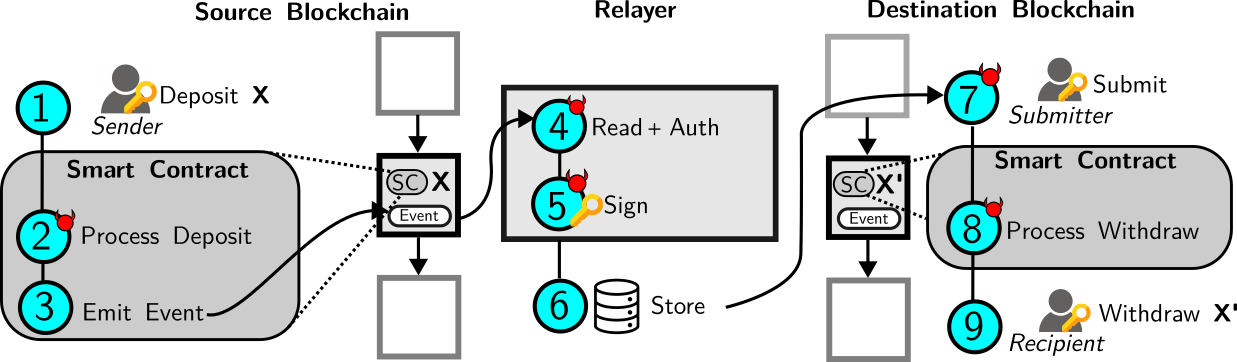
\includegraphics[width=0.8\textwidth]{fig/bridge_arch.pdf}
%%command for cropping pdf
%%gs -sDevice=pdfwrite -o bridge_arch_crop.pdf bridge_arch.pdf
\caption{Cross-chain token bridging and the different steps attackers can exploit to withdraw unbacked deposits.}
\label{fig:cross-chain}
\end{figure*}

\section{Background}
\label{sec:background}
% In this section, we start by providing an overview of blockchain technology. We then describe how cross-chain bridges work followed by the threat model we consider in this paper.
% In this section
We first give a brief introduction to smart contract blockchains
and cross-chain bridges. We then describe how bridges, under attack, collapse in
practice.

\subsection{Smart-contract Blockchains} Modern DeFi protocols (e.g.,
decentralized exchanges and lending protocols) are built on top
of ``smart-contract'' blockchains, like Ethereum. At their core, these chains, like
the original Bitcoin blockchain, are distributed ledgers that manage accounts
(public keys) and their balances (in native tokens like Ethereum's ETH). Users
interact with these chains by signing and broadcasting (to the distributed nodes
that make up the chain network) transactions that, for example, transfer
funds from their account (using the corresponding account private key) to
another user's account.

Ethereum, and the smart-contract chains it inspired since its release in 2015,
differ from Bitcoin by extending the ``simple'' distributed ledger with a smart
contract execution layer. A smart contract on Ethereum is an \emph{internal}
account---and, like a normal, \emph{externally owned} account (EOA), it has a
balance---that has associated \emph{code} (EVM bytecode), which implements the
smart contract's program logic, and \emph{storage}, which persists the program's
state across executions. Users interact with (i.e., execute) smart contracts
much like they do when transferring funds from their account: they sign a
transaction that encodes the smart contract to call (i.e., the contract address),
the particular function to execute, and the arguments to call the function with.
Instead of simply transferring funds from the user's account, then, executing
such a \emph{smart-contract call} transaction amounts to executing the smart
contract bytecode---and any smart contracts the contract itself calls.
    
% \begin{lstlisting}
% contract USDC{
%   mapping(account => amount) _balances;
%   event Transfer(from, to, value);
%   function transfer(to, amount) {
%     address from = msg.sender; // user
%     // ... validate user has enough balance
%     _balances[from] -= amount;
%     _balances[to] += amount;
%     emit Transfer(from, to, amount);
%   }

%   function mint(to, amount) {
%     _balances[to] += value;
%     emit Transfer(address(0), to, amount);
%   }

%   function burn(from, amount) {
%     // ... validate user has enough balance
%     _balances[from] -= amount;
%     emit Transfer(from, address(0), amount);
%   }

%   function safeTransferFrom(from, to, amount){ 
%     // ... transfer tokens; revert if failed
%   }
% }
% \end{lstlisting}


\begin{figure}[t]
    \centering
    \includegraphics[width=\columnwidth]{fig/usdc-contract-2sp.pdf}
    \caption{Simplified USDC ERC-20 Token Contract.}
    \label{fig:erc20}
\end{figure}


    

% \lstdefinestyle{myStyle}{
%     belowcaptionskip=1\baselineskip,
%     breaklines=true,
%     % frame=none,
%     % numbers=none, 
%     basicstyle=\footnotesize\ttfamily,
%     % keywordstyle=\bfseries\color{green!40!black},
%     % commentstyle=\itshape\color{purple!40!black},
%     % identifierstyle=\color{blue},
%     backgroundcolor=\color{gray!10!white},
%     language=Python,
% }

% \lstdefinestyle{customc}{
%   belowcaptionskip=1\baselineskip,
%   breaklines=true,
%   frame=L,
%   xleftmargin=\parindent,
%   language=Python,
%   showstringspaces=false,
%   basicstyle=\footnotesize\ttfamily,
%   keywordstyle=\bfseries\color{green!40!black},
%   commentstyle=\itshape\color{purple!40!black},
%   identifierstyle=\color{blue},
%   stringstyle=\color{orange},
% }


\subsection{ERC-20 Tokens}
One of the immediate applications of smart contracts---and to date still one of
most popular---is to create custom tokens (or coins).  To launch a new token, an
organization no longer needs to launch a new blockchain; they can instead deploy
a new contract that implements the ERC-20 token standard interface on a chain
like Ethereum and take advantage of existing on-chain infrastructure like
decentralized exchanges that make it easy to, for example, trade one kind of
token for another---both native tokens (e.g., ETH) and other tokens.\footnote{
    Most EVM chains, i.e., chains that use Ethereum's execution layer,
    follow Ethereum standards like ERC-20. Most non-EVM chains like Solana
    (which have different execution models) have similar standards (e.g., SPL
    tokens in Solana's case).
}

Figure~\ref{fig:erc20} shows a simplified variant of one such token
contract---the USDC \emph{stablecoin} contract.  This contract tracks
how many USDC tokens an account has and governs the spending of these
tokens (much like a bank governs bank notes).  For example, the
contract's \texttt{mint} function lets Circle (the company that owns
the USDC contract) mint new tokens into a user's account---e.g., after
receiving the corresponding payment from the user off-chain (in US
dollars, as USDC tokens are pegged to the US dollar).  The contract
exposes the ERC-20 interface that lets users (and smart contracts)
transfer tokens from their account by simply calling functions like
\texttt{safeTransferFrom}, and, in turn, use the tokens in any DeFi
protocol (e.g., lending the USDC to different markets, exchanging USDC
for ETH,
% buying NFTs using the USDC,
etc.). Finally, the contract's
\texttt{burn} function ``burns'' a token out of circulation---and
emits an event (Figure~\ref{fig:erc20-event}) that Circle's off-chain code looks for before allowing
a user to withdraw the corresponding USD fiat off-chain.

% \subsection{Blockchain Basics}
% In this section, we cover the basic concepts of blockchain technology, including blockchains, smart contracts, transactions, accounts, and tokens.

% \textbf{Blockchains.} A blockchain is a distributed ledger that stores data (e.g., account balance) in a transparent and tamper-proof manner. It consists of a chain of blocks, where each block contains a certain amount of data, a reference to the previous block (thus forming a chain), and other information such as timestamp. Blockchains are maintained by a network of nodes that validate data in the blocks and reach consensus on the state of the ledger.\alex{somehow have to mention Solana and Ethereum and others?}
% % It consists of a series of blocks that are linked together via cryptography (thus forming a chain) [65]. These blocks are immutable and can be used to store data (e.g., transactions). They are also maintained by a distributed network of nodes, removing the need of a central server. 

% \textbf{Smart Contracts.} Smart contracts are programs that can be executed. Typically, smart contracts are first written in high-level programming languages such as Solidity or Rust. Then, they are compiled into bytecode and deployed to the blockchain. Upon deployment, each smart contract is assigned a unique address and becomes immutable. After deployment, they can be executed based on the input provided and the logic programmed into the contract.

% % , compiled into bytecode, and deployed to the blockchain. The input and execution of smart contracts are all recorded on the blockchain. They 

% % are stored and executed on blockchains. They are used to encode business logic, enforce rules, and automate processes. Smart contracts are written in high-level programming languages, compiled into bytecode, and deployed to the blockchain. Once deployed, smart contracts are immutable and can be interacted with by sending transactions.

% % self-executing programs that run on blockchains. They are used to encode business logic, enforce rules, and automate processes. Smart contracts are written in high-level programming languages, compiled into bytecode, and deployed to the blockchain. Once deployed, smart contracts are immutable and can be interacted with by sending transactions.

% \textbf{External Owned Accounts.}  Externally owned accounts (EOAs) represent users and are controlled by private keys. Users can interact with other users or deployed smart contracts by initiating a transaction from their EOAs. To initiate a transaction, a user specifies the recipient (the address of an EOA or a smart contract), the amount of assets to transfer, and any additional input parameters required by the smart contract. 

% % are entities that can send and receive transactions on the blockchain. There are two types of accounts: externally owned accounts (EOAs) and contract accounts. EOAs are controlled by private keys and represent human users, while contract accounts are controlled by smart contracts and represent autonomous entities.

% % Accounts are entities that can send and receive transactions on the blockchain. There are two types of accounts: externally owned accounts (EOAs) and contract accounts. EOAs are controlled by private keys and represent human users, while contract accounts are controlled by smart contracts and represent autonomous entities.


% \textbf{Transactions.} A transaction is a instruction set constructed and signed by a user using their EOA. It typically includes several fields, such as the sender (the EOA that signs the transaction), the recipient (which can be an EOA or a smart contract), the amount of assets to transfer, and the input parameters required by a smart contract. Once signed, the transaction is broadcasted to the network and executed. After successful execution, the resulting state changes are recorded on the blockchain along with the transaction itself.


% \textbf{Tokens.} Every blockchain system has its own native token. For example, Ethereum has Ether (ETH), while Solana has Sol (SOL). In addition to native tokens, blockchains can also host other types of tokens. An example is ERC-20 tokens on Ethereum, which are smart contracts that follow a set of rules and standards. Of particular note, when a user transfers ERC-20 tokens, the ERC-20 token contract emits an event (a type of debug information recorded on the blockchain) that logs certain information. Figure 1 shows an example. The name of the event is Transfer, and the token contract that emits the Transfer event is tagged as USDC. The sender and recipient are represented by their addresses (0x68... and 0xF5..., respectively). The amount of tokens transferred is 212295874.

% \alex{maybe liquidity pool}


\subsection{Cross-Chain Token Bridges}
While smart contracts make it easy to launch new tokens without spinning up new
chains, there is no real shortage of new blockchains being deployed (almost weekly).  Indeed,
the modern blockchain ecosystem is a many-chain ecosystem.  Blockchains like
Avalanche, Base, and Solana have different design points---from cheaper ``gas''
execution costs, to higher throughput, lower latency, and different permission
models---that make them better suited for different classes of application.
This situation has resulted in applications that span many chains and cross-chain
infrastructure that ultimately (try to) allow users to, for example, buy
Dogwifhat NFTs on Solana using USDC tokens on Ethereum.

Core to these applications and infrastructure---and the focus of our work---is
the \emph{cross-chain token bridge}.  At a high level, a cross-chain token
bridge makes it possible for a user to ``transfer'' their tokens from one chain
(e.g., their USDC on Ethereum) to another chain (e.g., Solana) and then use the
transferred tokens on the destination chain (e.g., on a Solana exchange trading
USDC and Dogwifhat).\footnote{While some cross-chain bridges \emph{do} let users
transfer one kind of token (e.g., USDC on Ethereum) for a completely different
kind of token on the destination chain (e.g., Dogwifhat on Solana), these bridges
essentially fuse the cross-chain token bridge with an exchange (or swap). We
focus on token bridges not only because they are fundamental to other kinds of
bridges, but also because they have higher volume, more liquidity, and more
attacks.} Since smart contracts cannot make network requests or otherwise
access sate outside their own storage, a cross-chain token bridge consists of
smart contracts on both the source and destination chains, and off-chain
infrastructure that serves to relay the ``transfer'' call across the two
contracts.

\begin{figure}[t]
\centering
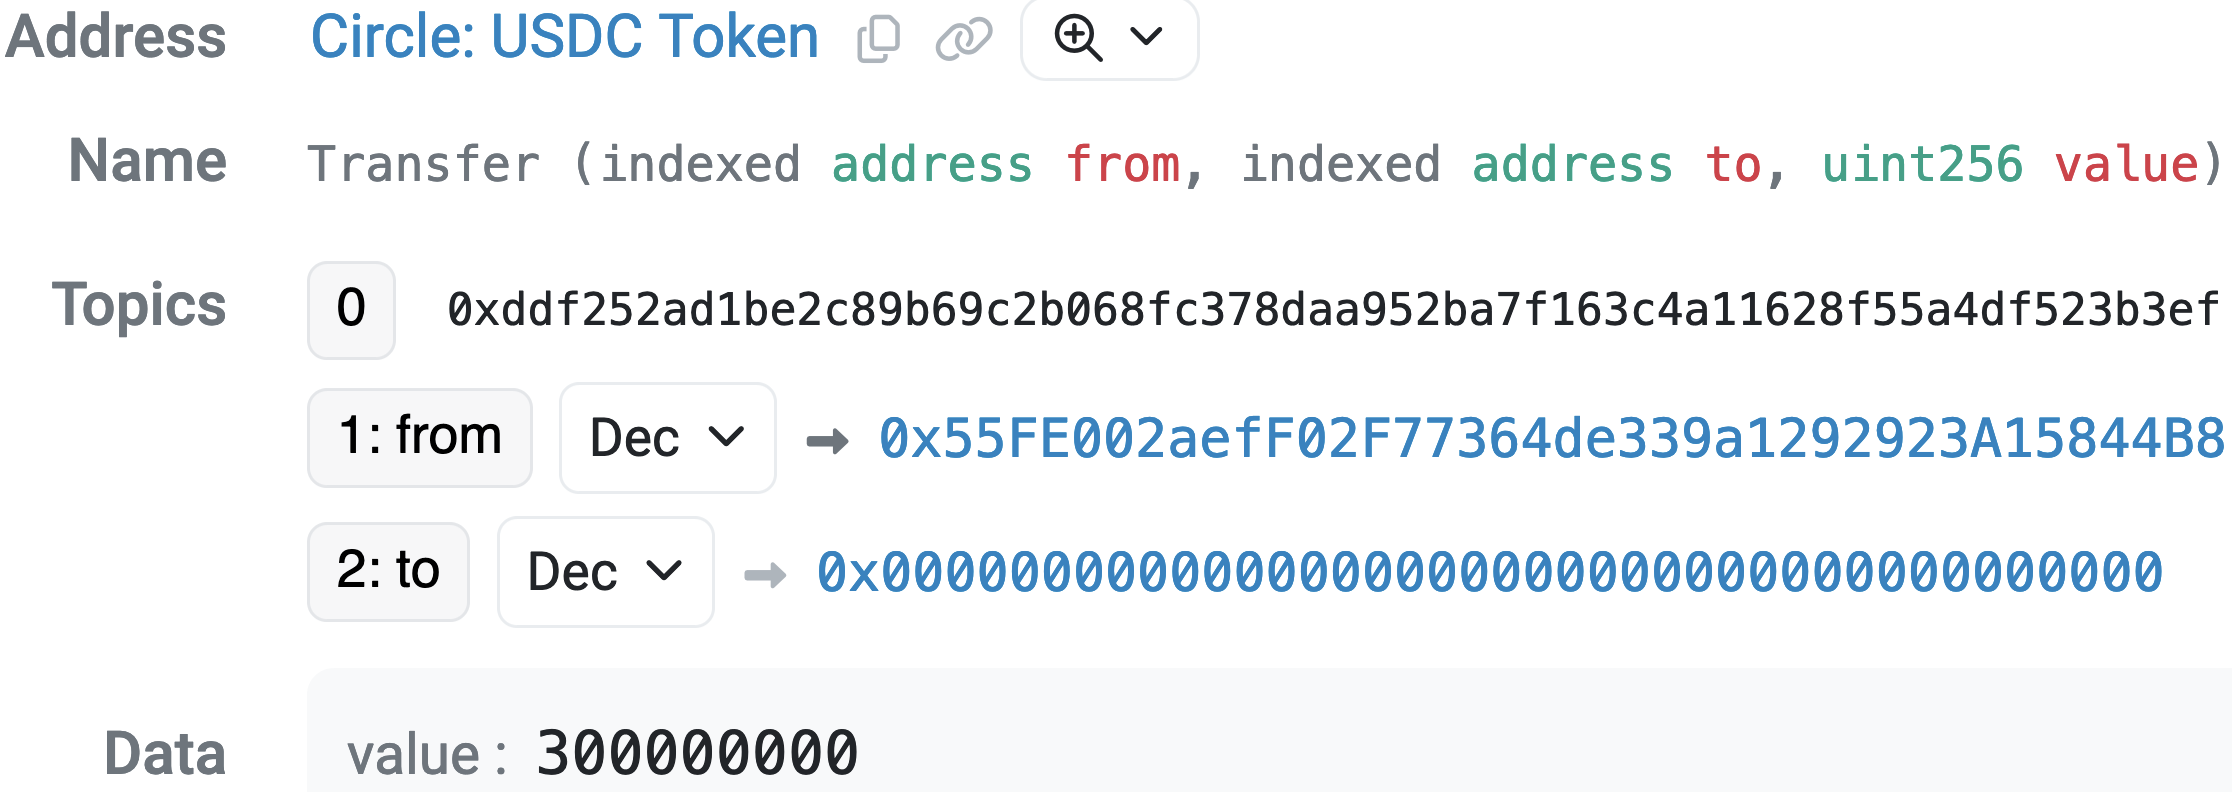
\includegraphics[width=\columnwidth]{fig/token.png}
\caption{Event Emitted by an ERC-20 Token (USDC).}
\label{fig:erc20-event}
\end{figure}

As Figure~\ref{fig:cross-chain} shows, a typical cross-chain token transfer,
i.e., a bridge transaction, consists three phases:

\textbf{1. Deposit (on source chain).}
To initiate a cross-chain token transfer, the user first calls the bridge's
contract on the source chain:
\begin{lstlisting}
deposit(address token, uint256 val, address to) {
  address from = msg.sender;  // user
  address to = address(this); // bridge contract
  // ... validate the ERC-20 token contract
  token.safeTransferFrom(from, to, val);
  emit Deposited(id++, token, from, to, val);
}
\end{lstlisting}
This contract function---a simplified version of the Qubit bridge deposit
function---processes the user's deposit (step 2) by validating the transfer request,
e.g., against a list supported tokens, and then transferring the user's ERC-20
tokens to the bridge contract---recall contracts are accounts with balances.
Then, the function emits an event (step 3) recording the user's deposit details
(including the deposit ID, the ERC-20 token contract address, the recipient on
the destination chain, and value).

\textbf{2. Off-chain relay.}
The emitted event is observed by an off-chain relayer in (step 4),
which constantly monitors the source blockchain.  The relayer first
verifies the authenticity of the deposit event.  If the event is
authentic, the relayer then produces a signed \emph{receipt}
endorsing the deposit (step 5) and, typically, stores the receipt off-chain (step
6).  Finally, this signed receipt is sent to the bridge's withdrawal contract
on the destination blockchain (step 7). Who submits the receipt varies across
bridges---some bridges submit the receipt on the user's behalf (in these cases, the
signed receipt is simply a signed contract-call transaction), while others give
users (and anyone willing to pay gas) the signed receipt and they, in turn,
submit the receipt to the withdrawal contract to complete the transfer. 

\textbf{3. Withdraw (on destination chain).}
The withdrawal contract on the destination chain first processes the withdraw
request by verifying the receipt and transferring the tokens to the recipient
(step 8). In (the simplified) Chainswap's withdraw case, for example, users call:
\begin{lstlisting}
withdraw(uint256 id, address token, address to, uint256 val, Signature[] sigs) {
  _chargeFee();
  // verify receipt
  require(received[id][to] == 0, 'withdrawn');
  for(uint i=0; i < sigs.length; i++) {
    verify_receipt(sigs[i], id, token, to, val);
  }
  received[id][to] = val; // mark as withdrawn
  token.safeTransferFrom(address(this), to, val);
  emit Withdraw(id, token, to, val);
}
\end{lstlisting}
This contract function first charges the caller a fee, then verifies the
deposit details against receipt---both that the deposit was not already
withdrawn and that the receipt signatures are valid---and finally transfers the
tokens to the intended recipient.  We consider a cross-chain transaction
complete when the asset is released to the recipient (step~9).

We expect every cross-chain bridge transaction to uphold the balance invariant:
the value (and kind) of the tokens withdrawn---the outflow---should equal the
value (and kind) of the tokens deposited---the inflow---minus the charged fees.
In practice, they do not.



% \subsection{Cross-Chain Bridges}
% In this section, we begin by providing an example of how a typical cross-chain transaction works. We then discuss the different variants of cross-chain bridges. 
% \subsubsection{A Typical Cross-Chain Transaction}
% Figure~\ref{fig:cross-chain} depicts a typical cross-chain transaction. Starting with the source blockchain, the sender (represented by their EOA) initiates a transaction to transfer assets to the bridge's deposit contract (step 1). The bridge contract then verifies that it has received the assets (step 2). Upon verification, the bridge contract emits an event to record the transfer (step 3). This event is observed by the relaying component (step 4), which typically resides outside and constantly monitors the source blockchain. The relaying component then verifies the authenticity of the event (step 5). If the event is authentic, the relaying component signs the message and stores the signature in a queryable database (step 6). A submitter on the destination blockchain then fetches the signed message from the database (step 7) and sends it to the bridge's withdrawal contract on the destination blockchain (step 8). The bridge contract then verifies the signature (step 9) and transfers the assets to the recipient (step 10). A cross-chain transaction is considered complete when the asset is released to the recipient (step 11).

% % Important things we need in this figure:
%     % source and dst amount
%     % how different vulnerabilities manifest
%         % source
%             % transfer in
%             % verify * emit
%         % relaying component
%             % observe
%             % signs
%         % dst
%             % retrieve & send
%             % verify
%             % transfer out
%     % Players
%         % Sender (in source)
%         % Relayer (in dst)
%         % Receiver (in dst)
    
    



% \subsubsection{Variants of Bridge Implementation}
% Beyond the typical cross-chain transaction described above, there are different ways to implement a cross-chain bridge. We discuss the following variants:

% \textbf{Asset Management.} There are two common ways funds can be released in step 10. The first model is the liquidity pool, which is commonly used when an asset already exists on both blockchains (e.g., USDC already exists on Ethereum and Polygon). Bridges start by creating liquidity pools, to which users can deposit assets and earn fees. When a withdrawal request is made, the bridge releases the funds from the liquidity pool as long as there is sufficient capital in the pool. The second model is mint-and-burn, which can be used regardless of whether the asset exists on the destination blockchain. In this model, the bridge contract mints new tokens on the destination blockchain, which act as representations of the assets on the source blockchain. When a withdrawal request is made, the bridge simply mints new tokens and sends them to the recipient. The recipient can then burn the tokens to receive the original assets on the source blockchain.



% \textbf{Submitter Privilege.} In the flow depicted in Figure~\ref{fig:cross-chain}, once the relaying component has signed the transaction, anyone can fetch the signed message and submit it to the destination blockchain. However, in practice, there is a variant where only privileged EOAs can act as submitters. In this variant, the authenticity of the message is verified by the presence of a privileged key. If bridges choose to operate in this way, they 
% typically simplify step 6 by directly storing the message without signing it.

% \textbf{Transaction Relay.} In the flow depicted in Figure~\ref{fig:cross-chain}, each transaction is relayed individually. In practice, transactions can also be relayed in batches or grouped into a Merkle tree. This approach can improve efficiency. However, while using a Merkle tree is more efficient, it also introduces additional complexity in step 9, where the bridge contract has to verify that a transaction is included in a Merkle tree.

% \textbf{Message Verification Mechanisms.} There are four different mechanisms to verify the authenticity of a message. Namely, external verification, optimistic verification, native verification, and local verification. The details of these mechanisms are not critical for this paper. We provide a brief overview of each model and refer the reader to \alex{cite} for more details. At a high level, external verification indicates that the relaying component resides outside both the source and destination blockchains. The legitimacy of a cross-chain transaction is attested by a third party (or a set of third parties). Native verification, on the other hand, indicates that the relaying component resides within the destination blockchain. In this model, the relaying component typically operates as a light client of the source blockchain and maintains enough information to verify the authenticity of a message from the source blockchain. Optimistic verification improves the efficiency of external verification by assuming that the majority of relayed transactions on the destination blockchain are valid. Instead of attesting to the validity of every transaction, optimistic verification only intervenes when a fraudulent transaction is detected. Finally, local verification means that the two parties involved in a cross-chain transaction (e.g., the sender and the submitter) must cooperate and collaborate for the transaction to succeed.

% \textbf{Token Swap Bridges.} In the above example, tokens released on the destination blockchain are backed by an equivalent amount of assets (less fee) on the source blockchain. However, in practice, bridges can also support token swap. In this case, an asset on the source blockchain is swapped for a different asset on the destination blockchain. For example, a user can swap 1 ETH for 100 USDC. The conversion rate is typically determined by the relaying component and may not be publicly disclosed. 

% \subsubsection{Variants of Verification Mechanism.}
% \textbf{External Verification.} In the most common case, the verification components resides outside both the source and destination blockchains. This is known as an externally verified bridge. The legitimacy and correctness of a cross-chain transaction is determined by a third-party (or a set of third-parties). Common ways to implement external verification include Multi-party Computation and Threshold Signature Scheme.\alex{cite}

% \textbf{Optimistic Verification.} Optimistic Verification improves on the efficiency of external verification by assuming that the majority of transactions are valid. Instead of attesting to the validity of every transaction, optimistic verification only intervenes when a dispute arises. This is known as an optimistic bridge. Concretely, every message that is passed to the destination blockchain is considered "pending" until the dispute window expires. The system relies on one or more honest watchers to dispute the message if it is incorrect. If no dispute arises, the message is considered valid.

% \textbf{Native Verification}
% Contrary to external verification, where the verification component resides outside the source and destination blockchains, the verification component in a natively verified bridge resides within the destination blockchain. Commonly, this is achieved by implementing a light client of the source blockchain within the destination blockchain, which maintains enough information for verifying the authenticity of a message. The security is guaranteed by the validators of the source chain. 


% \textbf{Local Verification}
% \alex{add citation. this is the most confusing one.}
% The basic idea is that the sender and the submitter
% have to cooperate and collaborate for a cross-chain transaction to succeed. 

\subsection{How Bridges Collapse}
In practice, attackers exploited bugs in all three components---the deposit
contract, the relayer, and the withdraw contract---and stole signing keys
to siphon hundreds of thousands of dollars.
%
Figure~\ref{fig:cross-chain} highlights the precise steps in the cross-chain
token transfer that attackers have historically exploited, including:
\begin{CompactItemize}
\item \textbf{Bugs in the deposit contract.} In step 2, the bridge contract
verifies that it has received the correct amount of assets before emitting an
event. Bugs in this verification logic could allow an attacker to deposit a
smaller amount of assets than what is recorded by the bridge in the event (step
3). For example, Qubit's \texttt{deposit} function  (see above) did not properly validate the token address. This bug allowed an attacker to pass \texttt{0} for the token address, so the contract function did not actually transfer any funds from the attacker's account but still emitted a \texttt{Deposit} event which allowed the attacker to withdraw actual tokens on the destination chain~\cite{qubit:rekt}.

\item \textbf{Bugs in the off-chain deposit verification.} In step 5, the
relayer verifies the authenticity of the deposit event emitted by the
bridge contract, including whether the event is emitted by the bridge's
designated contract.  Bridges that do not correctly verify
deposits would allow attackers to withdraw assets that are never deposited.
% ---and this 

\item \textbf{Stolen relayer (or submitter) keys.} In step 5, the relayer signs the deposit receipts which are then submitted to the withdrawal
contract as evidence of a valid deposit. If the relayer key is compromised
(e.g., as with the Ronin bridge~\cite{roninattack}) the attacker can forge a
valid receipt and then withdraw assets that were never deposited by calling
\texttt{withdraw} with the forged receipt.

The same is true for bridges that submit receipts on behalf of users---and
essentially restrict the \texttt{withdraw} callers to privileged submitter
accounts. The bridge submitter keys (step 8) have similarly been compromised
(e.g., as with AnySwap~\cite{anyswapattack}) and used to withdraw
unbacked deposits.

\item \textbf{Bugs in the withdraw verification.} In step 8, the bridge contract
verifies that the messages are signed by the relayer and have not
been replayed. Bugs in this verification logic (e.g., as we saw with
Wormhole~\cite{wormholeattack}) have allowed attackers to supply ``valid''
payloads that were not signed by the relayer and replay withdrawal
requests with valid deposit receipts that have already been withdrawn.
\end{CompactItemize}


% Liquidity Pool vs Mint-and-Burn. Example USDC on ETH and Polygon
% Verification Modes
% \subsection{Threat Model}
% In this section, we describe the attack surfaces that are in scope for this paper. Importantly, we assume that deposits and withdrawals are made through designated functions and that funds cannot be withdrawn through functions other than the designated withdrawal function(s). Given this setup, we consider the following attack surfaces:

% \textbf{Buggy Deposit Verification.} In step 2, the bridge contract verifies that it has received the correct amount of assets before emitting an event. Bugs in this verification logic could allow an attacker to deposit a smaller amount of assets than what is recorded by the bridge in the event (step 3).

% \textbf{Buggy Event Verification.} In step 5, the relaying component verifies the authenticity of the event emitted by the bridge contract, including whether the event is emitted by the bridge's designated contract. Failure to do so could allow an attacker to withdraw assets that were never deposited.

% \textbf{Compromised Relaying Key.} In step 6, the relaying component signs the message and stores the signature in a queryable database. If the relaying key is compromised, an attacker could forge a message and withdraw assets that were never deposited.

% \textbf{Compromised Submitter Key.} In step 8, some bridges operate in a privileged submitter mode, where the presence of the privileged submitter key is the only requirement to attest to the authenticity of a message. In this case, if the submitter key is compromised, an attacker could submit a forged message and withdraw assets that were never deposited.

%\textbf{Buggy Withdraw Verification.} In step 9, the bridge contract verifies that the messages are signed by the relaying component and have not been replayed. Bugs in this verification logic could allow an attacker to verify payloads that are not signed by the relaying component or to replay a message that has already been processed.

In this paper, we assume an attacker can exploit any of the aforementioned
components or otherwise control the relayer (or submitter) keys.
In the next section, we show that this attacker model and our simple
\emph{balance invariant checking} captures the largest attacks on cross-chain
bridges that have happened in the past.  In Sections~\ref{sec:live-audit} we show
that monitoring withdrawals and deposits on the source and destination chains
can be used to detect similar attacks in the future.  Finally, in
Section~\ref{sec:active-protect} we describe an \emph{announce-then-execute} bridge
design that enforces this invariant to prevent attacks before they happen.

We note that while our threat model captures a wide variety of vulnerabilities,
it is not exhaustive.  As with any detection system, an attack that violates one
of our assumptions (e.g., avoids violating the balance invariant by transferring
funds off-bridge or not having a withdrawal, subverts the transaction data used to validate the invariant,
etc.) might succeed.  
We similarly consider other smart contract bugs (beyond bugs in deposit and withdrawal functions) and account key compromises out of scope---and instead focus
on the cross-chain bridging aspects which are relatively less well understood.
As we show later, our model captures the largest attacks on
cross-chain bridges that have happened in the past and systems can use
it to prevent similar attacks in the future.


%% While our approach captures a variety of vulnerabilities, it is by no
%% means exhaustive. For example, a key assumption we make is that
%% withdrawal are done through designated withdraw functions. However, if
%% an adversary is able to compromise the key to account that holds the
%% funds for the bridge, they could simply transfer the funds to another
%% account and then withdraw them without going through the designated
%% withdraw function(s). Similarly, if an adversary is able to withdraw
%% funds by repurposing other functions (e.g., the deposit function), our
%% approach would not detect it. Moreover, if an attack transaction does
%% not involve a withdrawal, our approach would not detect it. Last but
%% not least, if an attack is somehow able to profit without breaking the
%% balance invariant, our approach would not detect it.  However, we
%% believe that our approach is a important first step in using
%% accounting principles to protect bridges from theft and that it can be
%% extended to address these and other vulnerabilities in the future.




%DIF <  \begin{table*}[h]
%DIF <    \begin{tabular}{l|llll|l|l}
%DIF <    \multirow{2}{*}{Consumer spyware apps} & \multicolumn{4}{c|}{Examples of Publicly Advertised Capabilities}                & \multirow{2}{*}{\# of permissions} & \multirow{2}{*}{Trenco Ranking} \\
%DIF <                                           & Location & SMS or call logs & Camera or microphone & Stealthiness &                                    &                                   \\
%DIF <    \hline
%DIF <    Flexispy                               & \checkmark        & \checkmark                 & \checkmark                   & \checkmark            & 46                                 & 117k                               \\
%DIF <    iKeyMonitor                            & \checkmark        & \checkmark                 & \checkmark                   & \checkmark            & 52                                 & 234k                              \\
%DIF <    Cerberus                               & \checkmark        & \checkmark                 & \checkmark                   &                       & 53                                 & 223k                              \\
%DIF <    mSPY                                   & \checkmark        & \checkmark                 & \checkmark                   & \checkmark            & 49                                 & 39k                              \\
%DIF <    Spyzie                                 & \checkmark        & \checkmark                 & \checkmark                   & \checkmark            & 38                                 & 961k                               \\
%DIF <    TheTruthSpy                            & \checkmark        & \checkmark                 & \checkmark                   & \checkmark            & 38                                 & 281k                              \\
%DIF <    Spyhuman                               & \checkmark        & \checkmark                 & \checkmark                   &                       & 44                                 & 213k                              \\
%DIF <    Hoverwatch                             & \checkmark        & \checkmark                 & \checkmark                   & \checkmark            & 35                                 & 90k                              \\
%DIF <    LetMeSpy                               & \checkmark        & \checkmark                 & \checkmark                   & \checkmark            & 15                                 & 2m                               \\
%DIF <    Spy24                                  & \checkmark        & \checkmark                 &                    & \checkmark                      & 49                                 & 464k                                \\
%DIF <    Talklog                                & \checkmark        & \checkmark                 & \checkmark                   &                       & 22                                 & N/A                              \\
%DIF <    Mobile-tracker-free                    & \checkmark        & \checkmark                 & \checkmark                   & \checkmark            & 40                                 & 62k                               \\
%DIF <    Spylive360                             & \checkmark        & \checkmark                 & \checkmark                   & \checkmark            & 34                                 & 2m                               \\
%DIF <    Spapp                                  & \checkmark        & \checkmark                 & \checkmark                   &                       & 46                                 & 569k                                \\
%DIF <    Highstermobile                         & \checkmark        & \checkmark                 & \checkmark                   &                       & 47                                 & 508k                              \\
%DIF <    \end{tabular}
%DIF <    \caption{Selection of 15 distinct off-store consumer apps, examples their advertised capabilities, \# of permission requested and their domains' Trenco ranking.\label{tab:apps_selected}}
%DIF <  \end{table*}
\DIFdelbegin %DIFDELCMD < 

%DIFDELCMD < %%%
%DIF < %
%DIF < % [app table in intro.tex to fine-tune placement]
%DIF < %
%DIFDELCMD < 

%DIFDELCMD < %%%
\DIFdelend \section{Spyware}

%DIF < % We select 15 distinct off-store consumer Android spyware apps from a large set of spyware
%DIF < % apps for our in-depth analysis (Table~\ref{tab:apps_selected}). We detail our
%DIF < % selection process in Section~\ref{subsec:app_selection}. In the process of
%DIF < % distilling the list of apps to study, we made several observations, such as
%DIF < % families of apps that are simply rebranded, among others. We provide more
%DIF < % information in Appendix~\ref{subsec:additional_observation}.
\DIFdelbegin %DIFDELCMD < 

%DIFDELCMD < %%%
\DIFdelend To provide context for our study, we first describe how spyware is
used in general and then describe how we selected the specific spyware
apps we investigate.

\subsection{Spyware Use}

Spyware enables an adversary to surreptitiously record the activities,
behavior, and location of a victim based on the victim's phone usage.
\DIFdelbegin \DIFdel{The spyware app has }\DIFdelend \DIFaddbegin \DIFadd{These invasive apps have }\DIFaddend a wide range of capabilities for
\DIFdelbegin \DIFdel{invasively
}\DIFdelend monitoring the victim, and \DIFdelbegin \DIFdel{does }\DIFdelend \DIFaddbegin \DIFadd{do }\DIFaddend so using existing Android APIs without
\DIFaddbegin \DIFadd{needing }\DIFaddend root access.
\DIFdelbegin \DIFdel{The goal of Section~\ref{sec:api-abuse} is to describe
in detail the various techniques that spyware apps use to implement
these invasive capabilities, as well as potential mitigations for
protecting users from such apps going forward.
}\DIFdelend 

\DIFdelbegin \DIFdel{The adversary performs a variety of steps to install and monitor the victim.  The }\DIFdelend \DIFaddbegin \DIFadd{To install these apps, the }\DIFaddend adversary first creates an account on the spyware\DIFaddbegin \DIFadd{'s }\DIFaddend web portal
interface and purchases a subscription, if required.  The adversary then
requires physical access to the victim's device to download and
install the spyware app.  When installing, the app requests an
extensive set of Android permissions as the basis for performing its
monitoring activity.  The adversary readily grants these permissions to
the app, a step which entirely undermines the Android app permission
model.  The adversary then signs in to the app on the device, typically
using the same credentials used by the web portal, and links the
victim\DIFaddbegin \DIFadd{'s }\DIFaddend device with the adversary's account on the spyware portal.

\DIFdelbegin \DIFdel{The }\DIFdelend \DIFaddbegin \DIFadd{Subsequently, the }\DIFaddend adversary no longer needs physical access to the victim's device, and
can remotely control the actions of the app via the \DIFaddbegin \DIFadd{online }\DIFaddend spyware portal.
The spyware app both passively collects data on the victim\DIFaddbegin \DIFadd{'s device }\DIFaddend (e.g.,
location, text messages, calls, etc.), and also allows the adversary to
perform on-demand remote actions like covertly recording audio and
video, taking app screenshots, etc.

\DIFdelbegin \DIFdel{The spyware app regularly uploads the data that it collects to servers
maintained by the spyware authors .  The adversary can then use the
spyware portal to view the data that the spyware app has exfiltrated
from the victim's device, loading the data from its servers.  While
spyware authors }\DIFdelend \DIFaddbegin \DIFadd{Although spyware authors }\DIFaddend exhibit tremendous effort and creativity in subverting
Android sandbox protections to implement their capabilities, many \DIFaddbegin \DIFadd{apps }\DIFaddend spend
much less effort in protecting the data that they \DIFdelbegin \DIFdel{upload }\DIFdelend \DIFaddbegin \DIFadd{exfiltrate }\DIFaddend and store on
their backend servers. \DIFdelbegin \DIFdel{The goal of }\DIFdelend \DIFaddbegin \DIFadd{Later, in }\DIFaddend Section~\ref{sec:data-leak} \DIFdelbegin \DIFdel{is to
describe the }\DIFdelend \DIFaddbegin \DIFadd{we
describe several }\DIFaddend vulnerabilities in spyware apps that put the victim's
data at risk to a third-party attacker.



\subsection{\DIFdelbegin \DIFdel{Spware }\DIFdelend \DIFaddbegin \DIFadd{Spyware }\DIFaddend App Selection}
\label{subsec:app_selection}

%% Our work focuses on off-store spyware apps since they request
%% a significant number of permissions (from 15 to 53, median 44), implement many
%% privacy-invasive capabilities (Section~\ref{sec:api-abuse}), and do not require root to function. In comparison,
%% apps that are available on the Google Play Store (typically these are apps
%% intended for consensual subordinate tracking of a child or employee) are less
%% likely to request dangerous permissions such as access to the camera, and
%% other permissions highly susceptible to abuse like
%% accessibility~\cite{feal2020angel}.


For our analysis, we chose 14 distinct \DIFaddbegin \DIFadd{leading }\DIFaddend consumer Android spyware
apps.\footnote{Often the same spyware app is available under multiple
  names.  Appendix~\ref{subsubsec:app_family} describes how we
  identify and avoid choosing duplicate apps.}  We focus on
Android-based spyware because most of the mobile spyware market
appears to be focused there. Since curated app stores do not permit
the sale of such apps, in practice they must be side-loaded, a process
that Apple does not support.  As a result, consumer mobile spyware only operates on ``rooted'' iPhones.  Rooting an iPhone can be a
technically involved operation (one popular guide to jailbreaking the
iPhone involves 41 distinct steps \cite{howToJailbreakIphone:online}) and one that can take significant
time to complete --- both requirements at odds with the broad,
non-technical customer base such apps are marketed to. \DIFaddbegin \DIFadd{We also focus on leading spyware apps as they are the apps that more people are exposed to and they are more likely to be innovative (new features could potentially bring them more customers).
}\DIFaddend 

%DIF < % We focus on Android since it has the largest smart phone market share~\cite{MobileOp2:online} and it supports sideloading apps that are not signed or downloaded via
%DIF < % the official Google Play Store.  We specifically focus on apps that do not
%DIF < % require root.  Since rooting breaks Android sandboxing and naturally offers
%DIF < % elevated permissions, such apps do not need to find creative ways to bypass
%DIF < % Android restrictions.
\DIFdelbegin %DIFDELCMD < 

%DIFDELCMD < %%%
%DIF < % Finally, we include apps that are popular and advertise a
%DIF < % rich set of capabilities while limiting our selection in order to dive deep into
%DIF < % each app.\alex{cite. Someone double checks the statements in paragraph.}
%DIF < % \geoff{not sure what feasibility means here?  also, this last sentence seems
%DIF < % redundant with text in the next paragraph?}
%DIFDELCMD < 

%DIFDELCMD < %%%
\DIFdelend In our selection process, we started with the 18 off-store spyware apps identified by Chatterjee et al.~\cite{chatterjee2018spyware}. We augmented our set of apps by taking the intersection of two major industry reports (\cite{esetandr4:online} and~\cite{Tekstalk86:online}) that listed spyware apps.\footnote{We take the intersection of both reports because (a) the definition of consumer spyware is vague; and (b) the collection process is ad-hoc and differs for each report. Apps in the intersection represent consensus among these disparate classifications.} Next, we sorted all the apps based on the Tranco ranking~\cite{pochat2018tranco} \DIFaddbegin \DIFadd{of their website domain }\DIFaddend (snapshot taken on May 5th, 2022)\DIFdelbegin \DIFdel{of their website domain}\DIFdelend .  We filtered out apps that were distributed via Google Play or broken (e.g., not reachable or no longer accepting payments). For apps that are rebranded versions of other apps, we consider them duplicates and \DIFdelbegin \DIFdel{do }\DIFdelend \DIFaddbegin \DIFadd{did }\DIFaddend not examine them separately (Appendix~\ref{subsubsec:app_family} details how we detect duplicate apps).

From the top 25 most popular apps, we identified 14 distinct apps which we used in our study. \DIFdelbegin \DIFdel{This set of apps }\DIFdelend \DIFaddbegin \DIFadd{The apps in this set }\DIFaddend are produced by a wide spectrum of vendors, with a broad array of capabilities, and cover the majority of apps identified in prior work~\cite{chatterjee2018spyware} (10 out of the 14 apps that are still alive). Moreover, we find significant overlap in the low-level technical implementation of spyware capabilities:  all but three techniques described in Section~\ref{sec:api-abuse} are discovered after the 5th app (Flexispy), and no new techniques are found after the 11th app (Spy24).\footnote{While we do continue to find different variants or implementation of the same technique, we view these as minor details.}  \DIFdelbegin \DIFdel{This suggests that this set of popular apps capture the }\DIFdelend \DIFaddbegin \DIFadd{The lack of new techniques discovered among less popular apps in our set suggests that the apps we study capture a }\DIFaddend representative set of techniques used in practice.


Table~\ref{tab:apps_selected} shows the list of spyware apps we chose, their website domain and its corresponding Tranco ranking, their \DIFaddbegin \DIFadd{web }\DIFaddend portal domain and its corresponding Tranco ranking, \DIFaddbegin \DIFadd{and }\DIFaddend their APK's \DIFdelbegin \DIFdel{version code and }\DIFdelend target SDK version \DIFdelbegin \DIFdel{, and their }\DIFdelend \DIFaddbegin \DIFadd{and }\DIFaddend package name. \DIFaddbegin \DIFadd{Table~\ref{tab:add_app_info} in Appendix~\ref{sec:additional_figures} provides additional information (version code and SHA-1 hash) about their APK files.
}\DIFaddend 




%DIF < % \geoff{the permissions column might be better placed into Table 2, but
%DIF < %   low priority at the moment}
\DIFdelbegin %DIFDELCMD < 

%DIFDELCMD < %%%
%DIF <  Commenting because section 4 explains the methodology.
%DIF < \subsection{Backend Vulnerability Discovery Methods}
%DIF < TBD
%DIF < \subsubsection{Threat Model}
%DIF < TBD
%DIF < \subsubsection{Experimental Setup}
%DIF < TBD
%DIFDELCMD < 

%DIFDELCMD < %%%
\DIFdelend %\input{spyware_app_selection}

%\input{spyware_api_abuse}

\section{SPYWARE ABUSE of ANDROID APIs}
\label{sec:api-abuse}

In this section, we \DIFdelbegin \DIFdel{detail }\DIFdelend \DIFaddbegin \DIFadd{explain }\DIFaddend how spyware apps implement various privacy invasive
capabilities using existing APIs supported by the Android OS.
%These different capabilities enable attackers to achieve various goals: monitor a user's online activities (e.g., the messages they send, the photos they take, etc.), abuse the device to spy on the user's activity in the physical world (e.g., using the victim's phone to silently record audio and video or track their location), stealthily spy on their victim without their knowledge or consent, and persistently conduct their spying over a long period of time.
We start by discussing our methodology for identifying these capabilities and uncovering their associated implementations.
We then summarize the set of basic capabilities \DIFaddbegin \DIFadd{(\S~\ref{subsec:features_enabled_by_permission}) }\DIFaddend that either do not require any permissions or are enabled just by acquiring permissions,
and group
all of the other capabilities that we study into three categories based on their goals: stealthily
\DIFdelbegin \DIFdel{collect }\DIFdelend \DIFaddbegin \DIFadd{collecting }\DIFaddend a victim's information \DIFaddbegin \DIFadd{(\S~\ref{subsec:data_gathering})}\DIFaddend , hiding the app's presence on the phone \DIFaddbegin \DIFadd{(\S~\ref{subsec:hiding_the_app})}\DIFaddend , and persistently
spying over a long period of time \DIFaddbegin \DIFadd{(\S~\ref{subsec:persistence})}\DIFaddend .
For each category, we
describe
each capability in the category and its associated implementations, and end
the category by discussing potential mitigations.
%We conclude this section with a short discussion.

%\grant{Suggestion for an extra overview sentence: These different features
%enable attackers to achieve four invasive goals: monitor a user's online
%activities (e.g., the messages they send, the photos they take, etc.), abuse the
%device to spy on the user's activity in the physical world (e.g., using the
%victim's phone to silently record audio and video or track their location),
%stealthily spy on their victim without their knowledge or consent, and
%persistently conduct their spying over a long period of time.} \grant{My
%suggested wording above is a bit clunky, but I think it would be helpful to
%structure these features in terms of slightly high-level goals that stalkers
%want to achieve (capturing different kinds of the victim's digital + physical
%activity, stealthily performing their spying, and being able to spy on the
%victim for long periods of time) and present an overview of this framing
%upfront.}

%We start by describing how we select the features and our methodology for
%uncovering implementations associated with each feature
%(Section~\ref{subsec:misuse_discovery}). Next, we present X features and their
%implementations, and discuss potential mitigation solutions
%(Section~\ref{subsec:api_abuse_results}).

% \begin{figure*}[h]
% \includegraphics[width=\textwidth]{figures/APIAbuse.pdf}
% \caption{Summary of features studied}
% \label{tab:feature_summary}
% \end{figure*}



\begin{table*}[h]
  \centering
    \DIFdelbeginFL %DIFDELCMD < \begin{tabular}{p{3.2cm}p{4.7cm}llllllllllllll}
%DIFDELCMD <       %%%
\DIFdelendFL \DIFaddbeginFL \begin{tabular}{p{3.0cm}p{4.7cm}llllllllllllll}
       \DIFaddendFL Category                                                &Capabilities                          &\rotatebox{90}{mSPY}  &\rotatebox{90}{Mobile-tracker-free}  &\rotatebox{90}{Clevguard}  &\rotatebox{90}{HoverWatch}  &\rotatebox{90}{Flexispy}  &\rotatebox{90}{Spyic}  &\rotatebox{90}{Spyhuman}  &\rotatebox{90}{TheTruthSpy}  &\rotatebox{90}{iKeyMonitor}  &\rotatebox{90}{Cerberus}  &\rotatebox{90}{Spy24}  &\rotatebox{90}{Spapp}  &\rotatebox{90}{Meuspy}  &\rotatebox{90}{Highstermobile}  \\
      \midrule
    \DIFdelbeginFL %DIFDELCMD < \multirow{11}{*}{\shortstack[l]{Basic Capabilities}}    %%%
\DIFdelendFL \DIFaddbeginFL \multirow{11}{*}{\shortstack[l]{Basic Capabilities (\S~\ref{subsec:features_enabled_by_permission})}}   \DIFaddendFL &Ambient Recording                     &                      &\checkmark                           &                 \DIFdelbeginFL %DIFDELCMD < \checkmark                 %%%
\DIFdelendFL &                            &\checkmark                &                       &\checkmark                &\checkmark                   &\checkmark                   &\checkmark                &\checkmark             &\checkmark             &\checkmark              &                                \\
                                                                                                     &Calendar                              &\checkmark            &\checkmark                           &\checkmark                 &\checkmark                  &\checkmark                &\checkmark             &\checkmark                &\checkmark                   &\checkmark                   &\checkmark                &\checkmark             &\checkmark             &\checkmark              &\checkmark                      \\
                                                                                                     &Call Logs                             &\checkmark            &\checkmark                           &\checkmark                 &\checkmark                  &\checkmark                &\checkmark             &\checkmark                &\checkmark                   &\checkmark                   &\checkmark                &\checkmark             &\checkmark             &\checkmark              &\checkmark                      \\
                                                                                                     &Clipboard                             &                      &\checkmark                           &                           &                            &                          &                       &                          &\checkmark                   &\checkmark                   &                          &\checkmark             &                       &                        &                                \\
                                                                                                     &Contacts                              &\checkmark            &\checkmark                           &\checkmark                 &\checkmark                  &\checkmark                &\checkmark             &\checkmark                &\checkmark                   &\checkmark                   &\checkmark                &\checkmark             &\checkmark             &\checkmark              &\checkmark                      \\
                                                                                                     &Info of Other Applications            &\checkmark            &\checkmark                           &\checkmark                 &\checkmark                  &\checkmark                &\checkmark             &\checkmark                &\checkmark                   &\checkmark                   &\checkmark                &\checkmark             &\checkmark             &\checkmark              &\checkmark                      \\
                                                                                                     &Location                              &\checkmark            &\checkmark                           &\checkmark                 &\checkmark                  &\checkmark                &\checkmark             &\checkmark                &\checkmark                   &\checkmark                   &\checkmark                &\checkmark             &\checkmark             &\checkmark              &\checkmark                      \\
                                                                                                     &Network Info                          &\checkmark            &\checkmark                           &\checkmark                 &\checkmark                  &\checkmark                &\checkmark             &\checkmark                &\checkmark                   &\checkmark                   &\checkmark                &\checkmark             &\checkmark             &\checkmark              &\checkmark                      \\
                                                                                                     &Phone Info                            &\checkmark            &\checkmark                           &\checkmark                 &\checkmark                  &\checkmark                &\checkmark             &\checkmark                &\checkmark                   &\checkmark                   &\checkmark                &\checkmark             &\checkmark             &\checkmark              &\checkmark                      \\
                                                                                                     &SMS or MMS                            &\checkmark            &\checkmark                           &\checkmark                 &\checkmark                  &\checkmark                &\checkmark             &\checkmark                &\checkmark                   &\checkmark                   &\checkmark                &\checkmark             &\checkmark             &\checkmark              &\checkmark                      \\
                                                                                                     &Shared Media Files                    &\checkmark            &\checkmark                           &\checkmark                 &\checkmark                  &\checkmark                &\checkmark             &\checkmark                &\checkmark                   &\checkmark                   &\checkmark                &\checkmark             &\checkmark             &\checkmark              &\checkmark                      \\
    \hline
\DIFdelbeginFL %DIFDELCMD < \multirow{4}{*}{\shortstack[l]{Data Gathering}}         %%%
\DIFdelendFL %DIF >     \multirow{4}{*}{\shortstack[l]{\S~3.3}} & \multirow{4}{*}{\shortstack[l]{Data Gathering}}         &Invisible camera access               &                      &\checkmark                           &\checkmark                 &\checkmark                  &\checkmark                &                       &\checkmark                &\checkmark                   &\checkmark                   &\checkmark                &\checkmark             &\checkmark             &\checkmark              &\checkmark                      \\
    \DIFaddbeginFL \multirow{4}{*}{\shortstack[l]{Data Gathering (\S~\ref{subsec:data_gathering})}}         \DIFaddendFL &Invisible camera access               &                      &\checkmark                           &\checkmark                 &\checkmark                  &\checkmark                &                       &\checkmark                &\checkmark                   &\checkmark                   &\checkmark                &\checkmark             &\checkmark             &\checkmark              &\checkmark                      \\
                                                                                                     &Invisible \DIFdelbeginFL \DIFdelFL{mic }\DIFdelendFL \DIFaddbeginFL \DIFaddFL{microphone }\DIFaddendFL access                  &                      &\checkmark                           &\checkmark                 &\checkmark                  &\checkmark                &                       &\checkmark                &\checkmark                   &\checkmark                   &                          &\checkmark             &\checkmark             &\checkmark              &                                \\
                                                                                                     &Accessing protected data               &\checkmark            &\checkmark                           &\checkmark                 &\checkmark                  &\checkmark                &\checkmark             &\checkmark                &\checkmark                   &\checkmark                   &\checkmark                &\checkmark             &\checkmark             &\checkmark              &\checkmark                      \\
                                                                                                     &Taking \DIFdelbeginFL \DIFdelFL{Screenshots                    }\DIFdelendFL \DIFaddbeginFL \DIFaddFL{screenshots                    }\DIFaddendFL &\checkmark            &\checkmark                           &\checkmark                 &\checkmark                  &                          &                       &\checkmark                &                             &\checkmark                   &                          &\checkmark             &\checkmark             &\checkmark              &                                \\
    \hline
\DIFdelbeginFL %DIFDELCMD < \multirow{3}{*}{\shortstack[l]{Hiding the App}}  %%%
\DIFdelendFL %DIF >     \multirow{3}{*}{\shortstack[l]{\S~3.4}} & \multirow{3}{*}{\shortstack[l]{Hiding the App}}  &Hiding app icon                       &\checkmark            &\checkmark                           &\checkmark                 &\checkmark                  &\checkmark                &\checkmark             &\checkmark                &\checkmark                   &\checkmark                   &\checkmark                &\checkmark             &\checkmark             &\checkmark              &                                \\
    \DIFaddbeginFL \multirow{3}{*}{\shortstack[l]{Hiding the App (\S~\ref{subsec:hiding_the_app})}}  \DIFaddendFL &Hiding app icon                       &\checkmark            &\checkmark                           &\checkmark                 &\checkmark                  &\checkmark                &\checkmark             &\checkmark                &\checkmark                   &\checkmark                   &\checkmark                &\checkmark             &\checkmark             &\checkmark              &                                \\
                                                                                                     &Launching a hidden app                &                      &\checkmark                           &                           \DIFaddbeginFL &\DIFaddendFL \checkmark                  &\checkmark                &\DIFaddbeginFL \checkmark             \DIFaddendFL &\checkmark                &\checkmark                   &\checkmark                   &\checkmark                &\checkmark             &\checkmark             &\checkmark              &                                \DIFdelbeginFL %DIFDELCMD < &                                %%%
\DIFdelendFL \\
                                                                                                     &Hide from recents screen              &\checkmark            &\checkmark                           &\checkmark                 &\checkmark                  &\checkmark                &\checkmark             &\checkmark                &                             &\checkmark                   &\checkmark                &\checkmark             &                       &\checkmark              &\checkmark                      \\
    \hline
\DIFdelbeginFL %DIFDELCMD < \multirow{2}{*}{\shortstack[l]{Persistency}}            %%%
\DIFdelendFL %DIF >     \multirow{2}{*}{\shortstack[l]{\S~3.5}} & \multirow{2}{*}{\shortstack[l]{Persistence}}            &Obscuring the uninstallation process  &\checkmark            &\checkmark                           &\checkmark                 &                            &\checkmark                &                       &\checkmark                &\checkmark                   &\checkmark                   &\checkmark                &\checkmark             &\checkmark             &\checkmark              &                                \\
    \DIFaddbeginFL \multirow{2}{*}{\shortstack[l]{Persistence (\S~\ref{subsec:persistence})}}            \DIFaddendFL &Obscuring the uninstallation process  &\checkmark            &\checkmark                           &\checkmark                 &                            &\checkmark                &                       &\checkmark                &\checkmark                   &\checkmark                   &\checkmark                &\checkmark             &\checkmark             &\checkmark              &                                \\
                                                                                                     &Creating "diehard" services           &\checkmark            &\checkmark                           &\checkmark                 &\checkmark                  &\checkmark                &\checkmark             &\checkmark                &\checkmark                   &\checkmark                   &\checkmark                &\checkmark             &\checkmark             &\checkmark              &\checkmark                      \\
    \hline
    \end{tabular}
    \caption{Summary of capabilities studied. A star denotes that an app implements a particular capability.
      %, otherwise we leave the corresponding cell in the table blank.
      \label{tab:feature_summary}}
  \end{table*}



\subsection{Methodology}
\label{subsec:misuse_discovery}


%% \geoff{I'm now thinking that we can use Section 2 to set the context:
%%   how spyware is used + our app selection process.  we'll then put the
%%   methodologies back into Sections 3 and 4.}

% Breaking into the vault: Privacy, security and forensic analysis of Android vault applications
% Transfiguring of an Android App Using Reverse Engineering
% Reverse engineering of mobile applications
% https://www.uit.edu.mm/storage/2020/09/No.-5.pdf
We gather a list of privacy invasive capabilities from two sources: (1)
capabilities advertised and offered by spyware apps; and (2) prior
academic papers and industry reports described in Section~\ref{sec:related_work} that look at how the Android API
can be used to achieve such unintended functionality.
Table~\ref{tab:feature_summary} summarizes the capabilities we study
and shows which spyware apps implement them.
To understand how the spyware apps implement their \DIFdelbegin \DIFdel{spyware }\DIFdelend \DIFaddbegin \DIFadd{nefarious }\DIFaddend capabilities, we \DIFdelbegin \DIFdel{take a reverse engineering approach}\DIFdelend \DIFaddbegin \DIFadd{reverse engineered and analyzed each app}\DIFaddend . Our approach consists of three steps.

\textbf{Preparation.} We acquire the latest APKs of spyware apps by directly downloading \DIFaddbegin \DIFadd{them }\DIFaddend from their websites. We use \texttt{APKTOOL}~\cite{ApktoolA72:online} to disassemble the APKs and obtain the corresponding manifest and smali code.\DIFdelbegin \DIFdel{We decompile the often obfuscated source code (more information on code obfuscation in Appendix~\ref{sec:apk_obfuscation}) to Java code with }\DIFdelend \DIFaddbegin \footnote{\DIFadd{Smali is a human-readable represenation of the Dalvik bytecode used by Android apps.}} \DIFadd{We also decompile the APK to Java source using }\DIFaddend \texttt{JADX}~\cite{skylotja9:online}. \DIFaddbegin \DIFadd{Identifiers and even strings in the Java code are often obfuscated, and Appendix~\ref{sec:apk_obfuscation} provides more details about the obfuscation used
by various apps.
}\DIFaddend 

\textbf{Manual Investigation.}
For each capability, we manually analyzed the app manifest and the decompiled Java code to determine how
each capability was implemented using the standard Android API: we manually located the API primitives associated with each capability, examined the relevant control flow, and confirmed that the primitives we identified were reachable. While we primarily used the decompiled Java code for
analysis, we reviewed the smali code when necessary (e.g., when a function fails
to decompile). Since the variable and method names were often obfuscated, we renamed them to human-readable ones as we examined the decompiled Java code (our naming annotations are available upon request).

Once we discovered an implementation for a particular capability and
the API primitives \DIFdelbegin \DIFdel{it uses, we used it to expedite the search process
in }\DIFdelend \DIFaddbegin \DIFadd{one app used, we expedited our search process
for }\DIFaddend other apps by searching for use of the \DIFaddbegin \DIFadd{same }\DIFaddend API primitives, and manually
reviewed the results to remove false positives. If this \DIFdelbegin \DIFdel{searching
}\DIFdelend \DIFaddbegin \DIFadd{API similarity
}\DIFaddend approach did not yield results, we reverted back to manually
inspecting the code.

We use two heuristics to guide our manual investigation process.
First, many apps can receive remote commands (e.g., using third-party
libraries such as Firebase~\cite{Firebase21:online}).  The method
responsible for dispatching remote commands is a useful top-down
starting place for identifying the underlying implementation (e.g.,
following the methods it calls in response to remote commands).  For
apps that do not receive remote commands, they operate as background
services to covertly collect user data. These background services
often are responsible for dispatching various tasks and contain useful
leads. Second, for any capability, there are limited ways to implement
it using Android API primitives\DIFdelbegin \DIFdel{(e.g., all audio recording needs to
configure the audio source), }\DIFdelend \DIFaddbegin \DIFadd{, }\DIFaddend and many of them are publicly
documented \DIFdelbegin \DIFdel{. }\DIFdelend \DIFaddbegin \DIFadd{(e.g., capturing audio through }\texttt{\DIFadd{MediaRecorder}}\DIFadd{). }\DIFaddend Searching for these API primitives in the code helps to
quickly locate methods associated with a capability. Additionally,
once we identified an implementation of a capability, we examined its
control flow in a bottom-up fashion to identify the operation that
would trigger its execution (typically leading back to dispatch
methods).

\textbf{Confirmation.} For each implementation of a capability (and
related API primitives) we discover, we \DIFdelbegin \DIFdel{verify that we correctly
identify it }\DIFdelend \DIFaddbegin \DIFadd{verified our analysis conclusions
}\DIFaddend by developing an app using the same API primitives and
testing it on a Pixel 4 phone running Android \DIFdelbegin \DIFdel{11 (code available upon
request). We also note that Android 12 was just released in October
2021 with some security enhancements}\DIFdelend \DIFaddbegin \DIFadd{11. We also installed and ran each spyware app to ensure the capabilities we observed were indeed enabled}\DIFaddend .
Since the majority of the apps we
study have been implemented \DIFdelbegin \DIFdel{to }\DIFdelend \DIFaddbegin \DIFadd{using }\DIFaddend Android APIs up to Android 11, we
discuss their implementations in that context. However, we also
discuss the impact changes in Android 12 can have on the spyware apps.

\DIFdelbegin \subsubsection{\DIFdel{Code Release}}
%DIFAUXCMD
\addtocounter{subsubsection}{-1}%DIFAUXCMD
\DIFdelend %DIF > \subsubsection{Code Release}
\DIFaddbegin \textbf{\DIFadd{Code Release.}}  \DIFaddend Our code that implements all the API
primitives discovered in this paper is available upon
request. Similarly, the annotated class and variable names are
available upon request (which can be used to reproduce our results
after \DIFaddbegin \DIFadd{independently }\DIFaddend acquiring the corresponding APK files). \DIFdelbegin \DIFdel{We cannot }\DIFdelend \DIFaddbegin \DIFadd{To avoid
potential copyright infringement risks, we do not }\DIFaddend provide the
decompiled and annotated source code \DIFdelbegin \DIFdel{as this would violate the
copyright of the spyware apps we studied}\DIFdelend \DIFaddbegin \DIFadd{itself}\DIFaddend .

%% We focus our discussion on Android 11 and earlier, and discuss the
%% impact of Android 12 when relevant. \alex{We need a machine that runs
%%   Android 12? Big enhancements include a persistent indicator and
%%   privacy dashboard}


%\subsection{Abusive and Non-abusive API Usage}
%\alex{maybe this is not necessary}
%We define Android API misuse as: any functionality that relies on using the
%Android platform API in ways that violate either Play Store policies or the
%clearly intended usage of the platform per the Android developer documentation.
%Broadly speaking, we focus on abusing API to: covertly collect private user or
%app data, hide app traces, and survive across reboots and kills.


% \subsection{Results}
% \label{subsec:api_abuse_results}
% We start by briefly discussing a set of features that are enabled after
% acquiring certain permissions. These features are only protected by
% permissions and many are not noticeable by users. Next, we detail how spyware
% apps implement features that allow them to exfiltrate data covertly, stay
% stealthy, and persist on the target device.

\subsection{Basic Capabilities}
\label{subsec:features_enabled_by_permission}
\DIFdelbegin \DIFdel{We start by describing various basic capabilities that allow spyware apps to
collect }\DIFdelend \DIFaddbegin \DIFadd{As seen in Table~\ref{tab:feature_summary}, all spyware apps support a large, common set of basic capabilities for collecting }\DIFaddend sensitive user data.
These capabilities either do not require any permission (e.g., clipboard) or are easily enabled after obtaining particular Android permissions (e.g., reading SMS messages, contacts, call logs, etc.). Spyware apps can obtain these capabilities simply by
requesting the associated permissions in the manifest \DIFdelbegin \DIFdel{and }\DIFdelend at installation or their first run.
Additionally, by design most of these capabilities
(except for location and ambient recording) do not provide any notification to
the user and are straightforward to implement.
\DIFdelbegin \DIFdel{Thus, as shown in Table~\ref{tab:feature_summary}, all spyware apps support at
least a large subset of these capabilities. 
}\DIFdelend 


\subsection{Data Gathering}
\DIFaddbegin \label{subsec:data_gathering}
\DIFadd{Spyware apps seek to stealthily collect a victim's information without being noticed. In this section, we describe how they covertly access the camera, the microphone, and protected data of other apps, as well as how they take screenshots all without the victim's knowledge.
}\DIFaddend 

\subsubsection*{Capability \#1: Invisible Camera Access}
\label{subsubsec:invisible_cam}
Spyware apps use \DIFdelbegin \DIFdel{the }\DIFdelend \DIFaddbegin \DIFadd{a device's }\DIFaddend camera to take pictures, record videos, and stream live
videos. To remain hidden \DIFdelbegin \DIFdel{to }\DIFdelend \DIFaddbegin \DIFadd{from }\DIFaddend the victim, spyware apps need to access the camera
without being noticed. The apps \DIFdelbegin \DIFdel{in our collection use three ways to achieve
hidden }\DIFdelend \DIFaddbegin \DIFadd{we studied use three methods to achieve
surreptitious }\DIFaddend camera access: (1) using an invisible preview; (2) intercepting raw
frames without a preview; and (3) using an invisible browser.

% (unique to Spy24);

% We start by briefly explaining how camera works. Readers who are interested in
% the details should refer to Android's developer
% guide~\cite{Cameraca74:online}. Android apps can capture images or videos by
% creating a camera capture session. To create a camera session, apps need to
% provide it with one or more output target buffers. One type of target buffer
% is SurfaceView, which can be used as a preview to display the image or video
% directly to the user. Other types of target buffers include ImageReader and
% SurfaceTexture, which are used for more advanced scenarios and not visible to
% users. If spyware apps uses SurfaceView as the target buffer, they need to
% hide the preview being displayed. This can be done by setting the preview size
% to 1x1.

% they can stay unnoticed by creating a SurfaceView that is not visible
% (typically of size 1x1).

\textbf{Invisible Preview}. One way to use the camera is to create a preview that displays an image or video to users. Once a preview is started, apps can take pictures or record videos. Benign apps (such as selfie apps) use a preview so that users can see the current status of the camera. Spyware apps, in contrast, seek to hide this preview \DIFdelbegin \DIFdel{, and do so by }\DIFdelend \DIFaddbegin \DIFadd{and use techniques that are well-documented in the malware literature (e.g., Yan et al.~\mbox{%DIFAUXCMD
\cite{yan2019understanding}}%DIFAUXCMD
): }\DIFaddend setting the preview to an invisible size (typically a 1x1 pixel) or \DIFdelbegin \DIFdel{be }\DIFdelend \DIFaddbegin \DIFadd{making the preview }\DIFaddend transparent.

\textbf{Raw \DIFdelbegin \DIFdel{Output }\DIFdelend \DIFaddbegin \DIFadd{Frames }\DIFaddend Without a Preview}.
Spyware apps can also access the output of the camera without displaying a
preview using advanced camera features supported by
Android~\cite{Cameraca74:online}. For example, apps can capture raw frames from
the camera with either an \texttt{ImageReade}r~\cite{Cameraca74:online} or
\texttt{SurfaceTexture}~\cite{SurfaceT78:online}, neither of which requires showing a
preview on the screen.
Benign apps (such as photo apps) use these
features for advanced operations such as frame-by-frame processing. Spyware
apps, on the other hand, use these features to capture raw frames, either saving
the frames locally or streaming the frames to a remote server, all without the
victim noticing. While the expectation for such advanced features is that the
processed frames will be displayed to users eventually (which is normally the
case for benign apps), this by no means is enforced. Finally, we note that four
apps rely on the third-party library WebRTC (or its variants) to achieve this functionality (WebRTC uses both \texttt{ImageReader} and \texttt{SurfaceTexture}).

%\geoff{does webrtc then use an ImageReader or SurfaceTexture?}\alex{fixed}

\textbf{Invisible Browser}. Unique to Spy24, this app uses an invisible
\texttt{WebView}~\cite{WebViewA25:online} (an in-app browser) with a 1x1 pixel size for
streaming live videos. While the browser may be invisible, the app can stream
full camera resolution to a Spy24 server.
%\geoff{Alex confirm?}\alex{correct}
\texttt{WebView} allows users to browse web content in an app while providing advanced
configuration options to developers. Spy24, in this instance, programmatically sets
the user agent, enables JavaScript, and disables the cache. This configuration
flexibility provided by \texttt{WebView} is necessary for streaming via a web browser.
%% as standard web browsers like Chrome have limited configuration
%% flexibility.\geoff{by hard to achieve, you mean hard to achieve
%% invisibly?}\alex{fixed}

Once the browser is configured, it accesses the camera via a JavaScript version
of WebRTC (loaded dynamically) and streams live video back to a Spy24 server.
This approach evades static analysis that examines API calls in the APK file, as
the JavaScript file is loaded during runtime.
Listing~\ref{lst:invisible_browser_code} shows a snippet of code that
demonstrates how Spy24 streams video with an invisible browser. First, it adds \DIFaddbegin \DIFadd{the 1x1 }\texttt{\DIFadd{WebView}} \DIFadd{as }\DIFaddend an overlay.  It then sets a specific user
agent to act as a trigger. Upon contacting the server, the \texttt{WebView} loads a
JavaScript file that activates the camera if the \texttt{WebView} has the specified user
agent.

\vspace{0.3cm}
\hspace{-0.1\linewidth}
%\begin{minipage}{0.5\textwidth}
\begin{lstlisting}[basicstyle=\small\ttfamily,caption={Code snippet that demonstrates how Spy24 streams live videos},label={lst:invisible_browser_code},captionpos=b,float=t]
// xml layout for the webview
<WebView id="@+id/wv" layout_width="1dp" layout_height="1dp"/>
// Java code that configures the webview
WebView webView = findViewById(R.id.wv);
webView.getSettings().setUserAgentString("some_user_agent");
// Javascript code that activates the camera when loaded by the webview
userAgent.includes('some_user_agent'){
  camera.start()
}
\end{lstlisting}

%\end{minipage}

%through Android's \texttt{camera2} framework~\cite{androidh66:online} or the
%deprecated \texttt{camera} framework~\cite.

%by building their customized camera implementation with the
%\texttt{android.hardware.camera2} framework (referred to as \texttt{camera2})
%or {CameraAn8:online} (referred to as \texttt{camera}). Both \texttt{camera2}
%and \texttt{camera} allow apps to capture pictures and videos.

%\texttt{camera} requires that a \texttt{Preview} must be started before
%pictures or videos can be taken~\cite{CameraAn8:online}. Spyware apps (e.g.,
%Flexispy) hide their preview by creating an invisible preview of size 1x1 as an
%overlay, a technique that has been documented in prior
%literature~\cite{yan2019understanding,pan2018panoptispy}. As an example, we
%provide more details on how Flexispy achieves invisible camera access. First,
%Flexispy access camera APIs through a foreground service, as apps running in
%the background cannot access the camera since Android 9 (API level
%28)~\cite{CameraAn8:online}. Furthermore, it adds a 1x1 \texttt{preview} to the
%screen through \texttt{WindowManager} as an \texttt{APPLICATION\_OVERLAY} (or
%\texttt{SYSTEM\_OVERLAY} before Android 6), which is protected by the
%permission \texttt{SYSTEM\_ALERT\_WINDOW}~\cite{WindowMa73:online}.
%Additionally, Flexispy will try muting the shutter sound when taking pictures
%or videos). However, we note that this is not possible in some countries (e.g.,
%Japan) due to legal concerns~\cite{HowcanIt38:online}. Finally, we observe that
%Flexispy attempts a series of different ways to access the camera if preceding
%methods fail.

%While the above approach still works for \texttt{camera2}, it is possible to
%stealthily access camera without a \texttt{Preview} with \texttt{camera2}. This
%technique has not been uncovered by any of the prior literature to the best of
%our knowledge. \texttt{camera2} provides more diverse ways of accessing camera.
%Apps need to specify one or more output target buffers to receive the raw
%image. One of the target buffers is \texttt{ImageReader}, which allows the
%spyware apps to copy the raw image into an array of bytes and save them to disk
%without launching a preview.

\subsubsection*{Capability \#2: Invisible Microphone Access}
\label{subsubsec:audio_recording}
Spyware apps use the microphone to covertly record
ambient sound, phone calls,
and voice calls (calls made in third-party apps like WhatsApp).
Ambient recording is enabled after acquiring the Android permission
to record\DIFdelbegin \DIFdel{, and }\DIFdelend \DIFaddbegin \DIFadd{; below }\DIFaddend we focus on how apps achieve phone \DIFaddbegin \DIFadd{call }\DIFaddend recording and voice call
recording.

\textbf{\DIFdelbegin \DIFdel{Call }\DIFdelend \DIFaddbegin \DIFadd{Phone call }\DIFaddend recording} on Android has evolved over time.
%% Prior to Android~6,
%% apps easily achieved call recording by setting the audio source to a specific
%% API value. From Android~6 to~8, an Android NDK workaround is required to capture
%% both uplink (Transmit) and downlink (Receive) audio source of a call. Since
%% Android~9, call recording is only possible through Microphone.  \geoff{this
%% paragraph summarizes the next, so we'll want to go with one or the other
%% depending on desired level of detail}
%
Prior to Android~6, apps could easily use \texttt{MediaRecorder} to
record phone calls~\cite{MediaRec53:online}.
% \geoff{parameter to what?}\alex{to voice call?} to \texttt{VOICE\_CALL}.
Specifying \texttt{MediaRecorder.AudioSource.VOICE\_CALL},
an app can receive both uplink and downlink audio
for a call. Since Android~6, \texttt{VOICE\_CALL} is protected by a permission
reserved for system apps and cannot be requested by third-party
apps~\cite{VOICECAL55:online}. Spyware apps (and other recording apps) use
native code via the Android NDK to circumvent this limitation, specifying
\texttt{VOICE\_CALL} by calling functions defined in
\texttt{libmedia.so}~\cite{ViktorDe77:online}.
%% ~\alex{Note, we studied the cited
%%   open-source implementation on Github instead of reverse engineering the native
%% code}.
Android~9 subsequently prevented this workaround by filtering out
unauthorized attempts to set \texttt{AudioSource}~\cite{coplukAC3:online,
  services10:online}.

After Android~9, spyware apps started recording phone calls using
Microphone, which nominally only captures uplink audio.  However, spyware apps
employ several workarounds to also capture downlink audio.  For instance, some
spyware apps turn on the speaker and turn off noise-cancelling during a phone
call so that the microphone can potentially capture downlink audio via the
speaker.
%% Related resources:
%% https://www.boldbeast.com/forum/topic1877-android-10-call-recording.html
%% https://nllapps.com/apps/acr/android9.htm
%% https://issuetracker.google.com/issues/112602629

%% \geoff{what is the difference between call
%% recording and voice call recording?}\alex{fixed in the beginning of this
%%   feature. Voice calls are calls made in apps like whatsapp}

\textbf{Voice call recording} became possible with
Android~10 \DIFdelbegin \DIFdel{by registering }\DIFdelend \DIFaddbegin \DIFadd{to apps that register }\DIFaddend as an accessibility service.  Prior to Android~10,
recording voice calls was not possible, as Android only allowed one app to
access input audio at a time~\cite{Sharinga60:online}.  Android~10 relaxed this
restriction, allowing two apps to access input audio concurrently if one of them
is an \texttt{AccessibilityService}.  This feature was intended to allow an
accessibility service to perform voice recognition, \DIFdelbegin \DIFdel{and }\DIFdelend \DIFaddbegin \DIFadd{however }\DIFaddend spyware apps quickly
abused it.  To detect that a voice call is active or a voice message is being
played, spyware apps use side-channels such as listening for specific
notifications triggered by voice calls or looking for specific actions (e.g.,
users clicking on the OK button to start the voice call) on the screen via
the accessibility interface.

\subsubsection*{Capability \#3: Accessing Protected Data\DIFdelbegin \DIFdel{in other Apps}\DIFdelend }
%DIF < \alex{maybe a new capability title?}
%DIF > \alex{This section needs a bit of help. Protected vs Private}
A core feature of spyware apps is the ability to collect data that they
are not supposed to read, which includes reading protected data of other apps (e.g.,
WhatsApp messages) and recording keystrokes to other apps. \DIFdelbegin \DIFdel{These capabilities are }\DIFdelend \DIFaddbegin \DIFadd{Accessing this data is }\DIFaddend normally
impossible as each app runs in its own sandbox. Spyware apps achieve these
capabilities primarily by abusing the accessibility permission which does not
require rooting, echoing prior literature~\cite{fratantonio2017cloak,
kraunelis2013malware, jang2014a11y, diao2019kindness, kalysch2018android,
huang2021a11y, naseri2019accessileaks} that investigates how accessibility can
be abused.

\textbf{Reading \DIFdelbegin \DIFdel{private }\DIFdelend \DIFaddbegin \DIFadd{protected }\DIFaddend data of other apps} can be performed in two ways: through
accessibility or notification. Most academic literature has focused on
accessibility, and only a few reports~\cite{VB2019Za6:online} have examined the
use of notification. Accessibility services are expected to read what is
rendered on the screen as they are designed to help disabled and impaired users.
Spyware apps abuse this capability to read information displayed by other apps
and extract sensitive information when an app (e.g., WhatsApp) is used.

Notification, on the other hand, allows spyware apps to read sensitive
information even if \DIFdelbegin \DIFdel{an }\DIFdelend \DIFaddbegin \DIFadd{the spyware }\DIFaddend app is not active. While reading from a notification has
limitations (e.g., a spyware app cannot read images), nine spyware apps abuse it.
Finally, we note that, like accessibility, both benign apps and malicious apps
make use of \DIFdelbegin \DIFdel{notification }\DIFdelend \DIFaddbegin \DIFadd{notifications }\DIFaddend as a side-channel for accessing information: benign
apps \DIFaddbegin \DIFadd{(an example is~\mbox{%DIFAUXCMD
\cite{ReadUnre55:online}}%DIFAUXCMD
) }\DIFaddend do so to avoid triggering the \DIFdelbegin \DIFdel{`Read Receipt' feature(}\DIFdelend \DIFaddbegin \DIFadd{``Read Receipt'' feature, }\DIFaddend which notifies the
sender if the recipient has read the message\DIFdelbegin \DIFdel{)
}\DIFdelend \DIFaddbegin \DIFadd{,
}\DIFaddend %\geoff{sorry, don't know what this is :-)}\alex{fixed}
of \DIFdelbegin \DIFdel{certain }\DIFdelend \DIFaddbegin \DIFadd{other }\DIFaddend apps (e.g., Signal \DIFdelbegin \DIFdel{) }\DIFdelend \DIFaddbegin \DIFadd{and WhatsApp), }\DIFaddend while malicious apps do so
purely to extract information.

\textbf{Recording keystrokes} is done via accessibility. Prior
work~\cite{fratantonio2017cloak,jang2014a11y,naseri2019accessileaks} has
demonstrated how the accessibility framework in Android can be abused for
recording keystrokes.
Spyware apps simply use the \texttt{getText} method, part
of Android's accessibility framework, to track all key presses from the user in
any app.
While there are built-in mechanisms to prevent \texttt{getText} from
reading sensitive information such as credentials (e.g., by setting
the attribute
\texttt{importantForAccessibility} to false), past
work~\cite{naseri2019accessileaks} has shown that these defenses are not
widely adopted. Additionally, \DIFaddbegin \DIFadd{mitigations like }\DIFaddend setting \texttt{importantForAccessibility} to
false also reduces the usability of benign apps such as screen readers.

%\damon{We should note that this defense would break screen readers.}\alex{fixed}

\subsubsection*{Capability \#4: Taking Screenshots}
\label{subsubsec:screenshot}
Spyware apps can also extract sensitive information by taking screenshots. We
observe two ways the apps in our set take screenshots: via
\texttt{MediaProjection} and \texttt{AccessibilityService}. For MediaProjection
to work, an activity is required~\cite{androidH20:online}. This approach is
nominally a challenge for spyware apps since they generally run as services and
do not have an activity. As a result, some spyware apps create temporary
activities that are transparent and not visible to users. These invisible
activities are then removed after the screenshot is taken.  Android~10 limited
apps that can start activities to a few scenarios~\cite{Restrict50:online}
(e.g., if an app is an accessibility service or has the \texttt{SYSTEM\_ALERT\_WINDOW}
permission). Such restrictions make it harder for spyware apps to use
\texttt{MediaProjection} to take screenshots, but still leaves a loophole as spyware apps
can register \DIFaddbegin \DIFadd{as }\DIFaddend an accessibility service and request the \texttt{SYSTEM\_ALERT\_WINDOW}
permission.
%\damon{this is vague, why does it not fully solve the problem?}\alex{fixed}

However, Android~11 (and later) has made it
simple for spyware apps to take screenshots by adding the
\texttt{takeScreenshot} API to \texttt{AccessibilityService}~\cite{Accessib97:online}.
This method requires no activity and is easy for spyware apps to implement.


\subsubsection{Mitigations}
\DIFdelbegin \DIFdel{Google }\DIFdelend \DIFaddbegin \DIFadd{Android }\DIFaddend has used a variety of approaches to mitigate some of the issues \DIFdelbegin \DIFdel{associated with permissions}\DIFdelend \DIFaddbegin \DIFadd{mentioned in this section}\DIFaddend .

\DIFdelbegin \DIFdel{One }\DIFdelend \DIFaddbegin \DIFadd{The first }\DIFaddend approach is to \DIFdelbegin \DIFdel{reduce the scope of granted permissions. For example,
}\DIFdelend \DIFaddbegin \DIFadd{pose additional restrictions on apps that seek to access certain information. One type of restriction is to require apps to be in a certain state: }\DIFaddend Android~10 restricted access to the clipboard \DIFdelbegin \DIFdel{~\mbox{%DIFAUXCMD
\cite{Privacyc52:online}
}%DIFAUXCMD
}\DIFdelend \DIFaddbegin \DIFadd{information
}\DIFaddend to apps that are either the default input
method editor or is the app that currently has focus\DIFaddbegin \DIFadd{~\mbox{%DIFAUXCMD
\cite{Privacyc52:online}}%DIFAUXCMD
}\DIFaddend . As a result \DIFdelbegin \DIFdel{, after }\DIFdelend \DIFaddbegin \DIFadd{of }\DIFaddend this
patch, none of the \DIFaddbegin \DIFadd{spyware }\DIFaddend apps were able to acquire clipboard information\DIFdelbegin \DIFdel{. We also note
that iKeyMonitor
%DIF < \geoff{(how do you like using a diff font for app names?)}
attempted to evade this restriction by trying to acquire focus with an
invisible }\texttt{\DIFdel{EditText}} %DIFAUXCMD
\DIFdel{of size 1x1. However, this attempt appears to be unsuccessful: both iKeyMonitor and our cloned implementation fail to read the clipboard. %DIF < % \geoff{how does this evade the restriction?  assume the
%DIF < % reader does not know what an EditText is}\alex{fixed}
}%DIFDELCMD < 

%DIFDELCMD < %%%
\DIFdelend \DIFaddbegin \footnote{\DIFadd{We are aware of a workaround~\mbox{%DIFAUXCMD
\cite{SolvedCl34:online} }%DIFAUXCMD
that can circumvent this restriction. However, it requires extensive user interaction and is not adopted by any of the spyware apps. We also note
that iKeyMonitor
attempted to evade this restriction by trying to acquire focus with an
invisible }\texttt{\DIFadd{EditText}} \DIFadd{of size 1x1. However, this attempt appears to be
unsuccessful: both iKeyMonitor and our cloned implementation fail to
read the clipboard.}}\DIFadd{. Another type of restriction is to require apps to possess additional permissions: besides requiring the permission to record audio, Android~10 further demands an app to be an accessibility service to capture audio input during phone calls. }\DIFaddend However, we note \DIFdelbegin \DIFdel{again that }\DIFdelend \DIFaddbegin \DIFadd{that permission-based restrictions are unlikely to be successful, as }\DIFaddend the abuser has physical access to the device \DIFdelbegin \DIFdel{, and as a result can grant permissions to the app to circumvent
Google's mitigations.
In addition to the }\texttt{\DIFdel{SYSTEM\_ALERT\_WINDOW}}
%DIFAUXCMD
\DIFdel{example from Capability \#4,
another example is how Android~9 limits the ability of
background apps to access the camera and microphone. Apps that want to
access a camera's data needs to run as a foreground service, which
shows a persistent notification that cannot be dismissed by
default. However, triggering this notification can be disabled by a
user, and spyware apps require that their notification be disabled
upon installation (Appendix~\ref{subsubsec:install_configure}). A
somewhat related example is how spyware apps record voice calls:
Android~10 requires that an app should be an accessibility service to
capture audio input via the microphone~\mbox{%DIFAUXCMD
\cite{Sharinga60:online}}%DIFAUXCMD
, which
spyware apps readily declare themselves to be.
}\DIFdelend \DIFaddbegin \DIFadd{and can grant arbitrary permissions.
}\DIFaddend 

%DIF > reduce the scope of granted permissions. 
%DIF >  For example,
\DIFaddbegin 

%DIF > % \geoff{how does this evade the restriction?  assume the
%DIF > % reader does not know what an EditText is}\alex{fixed}





\DIFaddend %Android also normally plays a shutter sound when a picture is taken. Spyware
%apps attempt to mute the shutter sound before taking the picture, which works
%in most scenarios (this is not possible in Japan due to legal
%concerns~\cite{HowcanIt38:online}). \geoff{by not possible, do you mean muting
%is disabled in Japan?} Finally, Android~12 introduces a persistent green dot
%indicator that signals to the user when an app is using the camera or
%microphone.  Its new privacy dashboard~\cite{AndroidD76:online} can also help
%mitigate the problem of covertly recording videos. To better alert users when
%an app is taking pictures (which happens quickly, making it harder for users to
%notice the indicator), Android can make the indicator appear for at least a few
%seconds regardless of the action taken.

A second approach is to provide a visible indicator to the user that cannot be
dismissed while a granted permission is being used by any app.  For example,
Android has a visible persistent indicator for location and screen recording
use, and Android~12 introduced a visible indicator for microphone and camera
use. Such an indicator confirms to the user when they expect it to be used, and
alerts the user when they do not.

This approach can also fail depending on the use case.  For example, a
\DIFdelbegin \DIFdel{consistent }\DIFdelend \DIFaddbegin \DIFadd{persistent }\DIFaddend indicator is useful to alert users to long-lasting actions
such as recording. However, a \DIFdelbegin \DIFdel{consistent }\DIFdelend \DIFaddbegin \DIFadd{persistent }\DIFaddend indicator is unlikely to be
helpful for sub-second operations (e.g., taking a screenshot and
taking a picture),
\DIFdelbegin \DIFdel{and it
is unlikely that users will notice the indicator due to the short-live nature of these operations.  }\DIFdelend %DIF > % as it is unlikely that users will notice the
%DIF > % indicator due to the short-live nature of these operations.
\DIFaddbegin \DIFadd{and users can sometimes miss these indicators (e.g., if the phone is
in a pocket or purse).  Moreover, benign use cases will also trigger
persistent indicators, which will then mask any simultaneous spyware
activity.  For example, the indicator for the microphone will be
displayed when a call is ongoing regardless of whether a spyware app
is performing call recording in the background or not.  In this case,
spyware apps can safely record calls in the background, as the
indicator is always on.  Indeed, sophisticated spyware can reduce
suspicion by carefully timing their actions (e.g., only performing an
action when the associated indicator is already triggered by another
app).
}\DIFaddend 

A third approach is to provide a convenient way for users to review the
permissions that have been granted to all installed apps.  Android~12 takes this
approach by introducing a privacy dashboard, which displays the
\DIFdelbegin \DIFdel{last 24-hour
accesses }\DIFdelend \DIFaddbegin \DIFadd{accesses in the last 24 hours }\DIFaddend to sensitive information such as location, microphone, and camera.
%% \geoff{which ... (describe the dashboard once here, no need when mentioned
%%   later)}\alex{fixed}.
While such a dashboard does require users to proactively
take action, it is a potentially useful tool for users to quickly identify
suspicious apps based upon the plethora of invasive permissions they have been
granted. We
recommend that all actions to access sensitive data should be added to the
privacy dashboard \DIFaddbegin \DIFadd{and users should be periodically notified of the existence of apps with excessive number of permissions}\DIFaddend .

Lastly, Android also employs various \DIFaddbegin \DIFadd{mechanisms that alert users of sensitive actions or potentially malicious activities. 
The most straightforward example is the deployment of Google Play Protect, which warns users when a potentially malicious app is being installed. As well, Android~9 requires a persistent notification for background apps that seek to access the camera and microphone: these apps need to run as a foreground service, which triggers a persistent notification that cannot be dismissed by the apps themselves. Finally, Android uses }\DIFaddend audio cues (e.g., a shutter sound) \DIFdelbegin \DIFdel{for
}\DIFdelend \DIFaddbegin \DIFadd{to notify users of }\DIFaddend operations such as audio and video recording. \DIFdelbegin \DIFdel{These }\DIFdelend \DIFaddbegin \DIFadd{Sadly, we note that all these mechanisms can fail, as they can be turned off either programmatically (e.g., }\DIFaddend audio cues normally can be
turned off \DIFdelbegin \DIFdel{programmatically }\DIFdelend after acquiring permissions to manipulate audio
settings\footnote{One exception is Japan, where muting the shutter sound when
taking pictures or videos is not possible due to legal
requirements~\cite{HowcanIt38:online}.}\DIFdelbegin \DIFdel{and as a result this mitigation does not work in most cases}\DIFdelend \DIFaddbegin \DIFadd{) or by a malicious user (e.g., as mentioned in Appendix~\ref{subsubsec:install_configure}, spyware apps require that their notification be disabled by the abuser upon installation)}\DIFaddend .


The research community has also proposed various defense mechanisms when
studying some of issues mentioned in this section. Huang et
al.~\cite{huang2021a11y}, for instance, seek to constrain accessibility misuse
with the assumption that the user is benign, which unfortunately does not hold
in the context of spyware apps.
%% \damon{give a succinct description of the
%%   solution in the citation.} \alex{fixed}
Another example is Petracca et
al.~\cite{petracca2015audroid}, who proposed requiring user approval before an
app can record to stop malicious apps from eavesdropping. However, we note that
this defense is unlikely to be successful as the adversary generally has physical access to the target device. On the one
hand, this defense will only work if user approval is requested every time,
which leads to significant usability issues. On the other hand, if user approval is
only requested once when an app tries to record, it is unlikely to be successful
as the abuser will have physical access to the phone and can grant the consent. Lastly, Yan et al.~\cite{yan2019understanding} developed a system for detecting overlay-based \DIFdelbegin \DIFdel{android }\DIFdelend \DIFaddbegin \DIFadd{Android }\DIFaddend malware. However, their \DIFdelbegin \DIFdel{approach does }\DIFdelend \DIFaddbegin \DIFadd{system is deployed on an Android app store and does not }\DIFaddend defend against spyware apps \DIFdelbegin \DIFdel{from being }\DIFdelend \DIFaddbegin \DIFadd{that are }\DIFaddend sideloaded.
%system was integrated into T-Market, an Android app store, and could not stop spyware apps from being sideloaded.

%% \geoff{the consent is only needed on install like a permission, or when an app
%% triggers recording during runtime?  sounds like the former but want to be
%% sure}\alex{fixed}

%\textbf{Mitigation.} Mitigating the issue of permissions enabling
%privacy-invasive functionality is challenging since benign apps often require
%these permissions to implement useful functionality.  The problem is made more
%challenging since a benign app (e.g., backup apps) can be abused for malicious
%purposes (e.g., data exfiltration), and there exists no reliable method to
%determine if the intention is malicious or benign~\cite{mayrhofer2021android}.
%Furthermore, abusers have physical access to the device, rendering existing
%solutions unusable.

%example is restricting access to sensitive information such as location and
%clipboard data.

%\grant{I suggest that we change the term ``data exfilitration'' to something
%like ``data capture''.  I think exfiltration will typically be interpreted as
%the process of siphoning the data off of the device and to an external source,
%but the features/capabilities below seem to be just about capturing/recording
%different data?  } This section contains a list of features supported by
%spyware apps to covertly exfiltrate data without being noticed.

%\grant{Something to consider in this section: there's a mix of different
%messages happening in this Data Exfiltration subsection: (1) we're giving an
%overview of the different kinds of data stalkerware apps can spy on, (2) we're
%highlighting that some of it can be done steathily, (3) we're talking about how
%apps get some of this data by cleverly breaking different kinds of separation
%boundaries (i.e., technical means to get functionality that they shouldn't be
%able to get).  Half of the features in this subsection seem to emphasize point
%(2) and the other half seem to emphasize point (3), which makes this data exfil
%section seem less unified on a conceptual level (e.g., is the main thing I
%should care about that that they capture X, Y, Z kinds of data? that they can
%do so stealthily? that they violate app separation mechanisms?).  I wonder if
%we could reframe the low-level wording in each feature to somehow make all of
%them about violating/bypassing user consent?  In other words, the overall
%message of this subsection is: (a) stalkerware apps want to collect information
%about users digital and physical activity (visual/audio/text/location) but (b)
%in order to collect this kind of sensitive information, an application
%typically needs to require consent either by the user (to use physical sensors
%like camera/microphone or to allow access to other applications/phone data).
%Here we analyze how attackers are able to get this data without any explicit
%consent by the users (we can still keep most of the content the same, with some
%small wording tweaks to make the stealthy spying features about bypassing
%consent for physical sensor access and the private data/screenshot features
%about bypassing consent for data/cross-app access).}

%\textbf{Mitigation.} Past literature~\cite{pan2018panoptispy,
%petracca2015audroid} has reported the potential risks of abusing the microphone
%to spy on users. Petracca et al.~\cite{petracca2015audroid} proposed requiring
%user consent before an app can record \geoff{the consent is only needed on
%install like a permission, or when an app triggers recording during runtime?
%sounds like the former but want to be sure}, which is unlikely to be successful
%in the context of IPV as the abuser will have physical access to the phone and
%can grant the consent. \geoff{we might discuss Android mitigations first (which
%exist), then what researchers have proposed}
%
%Android also has several defenses. First, Android by default plays a sound when
%a recording starts, but this audio cue can be disabled programmatically.
%Android~10 further requires that an app should be an accessibility service to
%capture audio input via the microphone~\cite{Sharinga60:online}, which spyware
%apps readily declare themselves to be.  As mentioned above, Android~12
%introduces a persistent visible indicator (green dot) that signals users when
%an app is using the camera or microphone as well as a privacy dashboard for
%reviewing permissions granted to all installed apps~\cite{AndroidD76:online}.
%While these features do not prevent spyware apps from recording calls, they do
%prevent them from doing it surreptitiously --- a significant step towards
%mitigation.

%\textbf{Mitigation.} Mitigating the abuse of accessibility or notification is
%challenging as there is no automated way to differentiate the intention of an
%app that is reading data. Huang et al.~\cite{huang2021a11y} proposes a
%framework for restricting accessibility services, but we note that this
%approach is unlikely to be successful in the context of spyware apps as they
%assume the user is benign. One potential solution is to show a persistent
%indicator for accessibility services when they are actively reading data and
%add accessibility services to the new privacy dashboard.\alex{i dont know what
%is in there} \geoff{the indicator has to be consistent with user accessibility
%(e.g., a green dot is not goin to help blind users)}

%\textbf{Mitigation.} Prior work~\cite{pan2018panoptispy} has overlooked using
%screenshots to violate privacy. The authors consider this functionality out of
%scope as Android displays a persistent indicator when the screen is being
%recorded. Due to Android's use of an indicator, most spyware apps only use
%MediaProjection to take screenshots (instead of live streaming the screen).
%Since taking a screenshot is a sub-second operation, it is unlikely that users
%will notice the indicator. Instead, we recommend that Android display the
%indicator for a few seconds regardless of the duration of the action. We also
%recommend adding the screen capture permission to the new privacy
%dashboard\alex{i dont know what is in there}.



\subsection{Hiding the App}
\DIFaddbegin \label{subsec:hiding_the_app}
\DIFaddend % This section details a list of features used by spyware apps to hide their
% activities and prevent users from discovering them.
In addition to surreptitiously spying on victims, spyware apps also use a
variety of methods to keep the existence of the app hidden from the victims.
% prevent their app from being enumerated to the user.  This section details a
% list of features used by spyware apps to hide their activities and prevent
% users from discovering them.
These tactics include hiding the app icon from the app launcher, launching a
hidden app, and hiding from the Recent screen.
%% \damon{We probably need to explain
%% some of this terminology since people might not know what the app launcher or
%% app list are conceptually. We might want to include a figure with examples of
%% these terms?} \grant{I made a slight tweak to the wording here, because I was
%% initially confused by why we have a separate stealthiness section when all of
%% the features in the previous section discuss how they steathily capture user
%% data. What this section really is about is making it so that the user cannot
%% find the app itself (rather than about having the app's functionality run
%% stealthily). The wording in my edit is not quite there yet (I'd like to make the
%% distinction more crisp, but this is minor wording/clarity stuff).}\alex{fixed}

\begin{figure}[t]
\centering
\includegraphics[width=0.95\columnwidth]{figures/app_launcher_wifi.pdf}
\caption{App launcher that displays app icons.
The Spyhuman app installed itself as the innocuous ``Wi-Fi'' icon.}
\label{fig:app_launcher}
\end{figure}

\subsubsection*{Capability \#5: Hiding App Icon}
\label{subsubsec:hide_icon}
To hide their presence,
% and make it harder for the users to noticing them,
spyware apps hide their app icons from the app launcher that lists the available
apps~\cite{whataret1:online}. Figure~\ref{fig:app_launcher} shows an example of
the app launcher, and 13 of the 14 spyware apps in our study include code to hide their
app icons from the app launcher using two methods:
% Specifically, we observe two ways to hide app icon from the app launcher:
(1) hiding the app icon at runtime, and (2) specifying no launcher activity.
% LEANBACK\_LAUNCHER~\cite{IntentAn39:online} instead of LAUNCHER.
%% \damon{again people likely do not know this terminology, such as app
%% drawer.}\alex{fixed}

\textbf{Hiding the app icon at runtime} can be implemented by invoking
the method \texttt{setComponentEnabledSetting()} and disabling the
launcher activity.  Previous work~\cite{shan2018self} examined hiding
app icons in this way, and this approach works on devices that run
Android 9 or below. An activity of category \texttt{LAUNCHER}
indicates that it should be displayed in the app
launcher~\cite{IntentAn33:online}, and disabling the launcher activity
removes the app icon from the app launcher.  Since the app is no
longer displayed in the app launcher, though, spyware apps need a
different way to launch themselves. We detail different ways to launch
apps that are not present in the app launcher in Capability \#6 below.

Since Android~10, an app's icon will appear in the app launcher even
if the launcher activity is disabled at runtime. In reaction to this
change, most spyware apps now use innocuous names and icons to
disguise the spyware app, such as ``Wi-Fi'' (\DIFaddbegin \DIFadd{as }\DIFaddend in Figure~\ref{fig:app_launcher}), ``SyncService'' and
``InternetService''.\footnote{iKeyMonitor even offers the ability to
  build apps that have customized icons and names.} Overall, \DIFdelbegin \DIFdel{13 of the
14 }\DIFdelend \DIFaddbegin \DIFadd{11 }\DIFaddend apps hide their icons in this way.


% Feature \#6 below.  Previous work~\cite{shan2018self} examined hiding app
% icons in this way and this method of hiding app icon at runtime does not work
% in Android 10 and later. \geoff{a bit awkward...we should rework this and the
% previous paragraph to phrase it in terms of up-to-Android~10}.

\textbf{Specifying no launcher activity} lets spyware apps hide app
icons even in the latest Android 12. While the patch introduced in
Android 10 effectively stopped apps from hiding their icons at
runtime, it still leaves a loophole. \DIFdelbegin \DIFdel{Apps that meet }\DIFdelend \DIFaddbegin \DIFadd{An app that meets }\DIFaddend any of the
following three requirements can still hide their icon from the
launcher~\cite{Launcher79:online}: (1) it is a system app; (2) it does
not request any permissions; or (3) the app does not have a launcher
activity that is enabled by default (a launcher activity has an intent
containing the \texttt{ACTION\_MAIN} action and the
\texttt{CATEGORY\_LAUNCHER} category). Spyware apps abuse the third
requirement and hide their app icons by specifying no launcher
activity.\DIFaddbegin \footnote{\DIFadd{We note that, for a short period of time (Android 10 builds r1 to r14~\mbox{%DIFAUXCMD
\cite{Launcher48:online}}%DIFAUXCMD
), the third requirement was ``the app does not have any components'', which should stop the abuse described in this section (as spyware apps cannot operate without components). Unfortunately, this requirement was changed to the current form since Android 10 build r15.}\label{footnote:hide_icon}}
\DIFaddend 

We observe two spyware apps (Spy24 and Meuspy) that implement this
technique: Spy24 only has an activity with an intent containing action
\texttt{ACTION\_MAIN} and \texttt{LEANBACK\_LAUNCHER} (used by TV
apps); Meuspy only has an activity with an intent containing
\DIFaddbegin \DIFadd{the }\DIFaddend \texttt{ACTION\_MAIN} action.
% \alex{maybe we dont need the technical details here?}
Since both apps do not have an icon displayed in the app launcher,
% and can be installed and run properly on an Android phone,
they cannot easily be started by a normal user.  As a result, both
Spy24 and Meuspy use a loader to start the app (as described in
Appendix~\ref{subsubsec:install_configure}).

We have disclosed the abuse of the \texttt{LEANBACK\_LAUNCHER} intent
on phone apps to Google, and Google determined that
this abuse was not a security vulnerability.\DIFaddbegin \footnote{\DIFadd{They note that such ``icon hiding'' is against Google Play }\emph{\DIFadd{policy}}\DIFadd{, but since none of the apps we studied are deployed via Google Play this restriction has no impact.}}
\DIFaddend 

\subsubsection*{Capability \#6: Launching a Hidden App}
\label{subsubsec:launch_hidden_app}
When spyware apps hide by excluding themselves from the launcher
(Capability \#5), they need an additional mechanism to launch.\DIFaddbegin \footnote{\DIFadd{We note that two apps, mSPY and Clevguard, do not provide ways to unhide icons even though they can hide icons.
These two apps do not interact with users after hiding their icons upon installation, and configuring them post-installation is done remotely through the web portal. Additionally, while mSPY has implemented functions to unhide its icon via a remote command, it does not offer such an option on its web portal.}}  \DIFaddend One
mechanism is to provide a way for the abuser to unhide the app icon on
demand.  We observed two ways apps unhide their app icon: by sending a
command from the web portal or an SMS text from a phone. Apps can
monitor SMS text messages by acquiring the \texttt{RECEIVE\_SMS}
permission, and can receive commands using third-party libraries such
as Firebase~\cite{Firebase21:online}.  Once launched, the abuser
can send a similar command to hide the app icon again.

A second mechanism is to have apps
launch themselves based on an external trigger,
keeping the app icon hidden.
This mechanism is generally achieved by
receiving a predetermined signal from another app in the system via the Intents
abstraction. We observed \DIFdelbegin \DIFdel{apps using two }\DIFdelend \DIFaddbegin \DIFadd{two main }\DIFaddend ways to do this \DIFaddbegin \DIFadd{signalling}\DIFaddend : (1) entering a hidden code via
Android's dial pad, which is the predominant approach; and (2) entering a URL in
the browser.

Apps that launch by entering a hidden code with Android's dial pad
register a system broadcast receiver that listens for the
\texttt{NEW\_OUTGOING\_CALL} intent. This intent is automatically broadcast by
the system when there is an outgoing call, which in turn invokes the receiver
registered by the app.  Apps can monitor outgoing dialed numbers and launch
themselves after a specific code (e.g.,
\texttt{*1234\#}) is entered in the dial pad.
%% \damon{might want a little
%% more explanation of why it is straightforward to implement the first two and not
%% the last one.}\alex{fixed}
Launching an app via a browser URL can be done by
adding an intent filter for a specific URL (e.g.,
\texttt{www.myapp.com/launch}) in the manifest (e.g., as described in~\cite{CreateDe16:online}). This intent filter specifies how to route an
intent that has the matching URL.

Unique to Hoverwatch, \DIFdelbegin \DIFdel{it }\DIFdelend \DIFaddbegin \DIFadd{besides implementing the mechanisms mentioned above, it also }\DIFaddend supports launching itself by entering a
code through a widget: a miniature app view that can be embedded in other
applications such as the home screen~\cite{Appwidge49:online}. Upon installation,
Hoverwatch creates a widget that has an \texttt{EditText} control that takes user input. If users
enter the correct code, it launches itself.
% \alex{screenshot?}



\subsubsection*{Capability \#7: Hide From the Recents Screen}

Android lists recently accessed activities and tasks in the Recents
screen~\cite{Recentss9:online} (see Figure~\ref{fig:recents_screen} for an
example). Past literature~\cite{shan2018self, zhou2020demystifying} has
documented that the \texttt{android:excludeFromRecents} attribute can be abused
to hide app activity, and this abuse is trivial to implement. It can be done via
setting the \texttt{android:excludeFromRecents} attribute to true for relevant
activities in their manifest~\cite{activity72:online} or programmatically adding
the flag
\texttt{FLAG\_ACTIVITY\_EXCLUDE\_FROM\_RECENTS}~\cite{IntentAn90:online} to an
activity.

\begin{figure}[t]
\centering
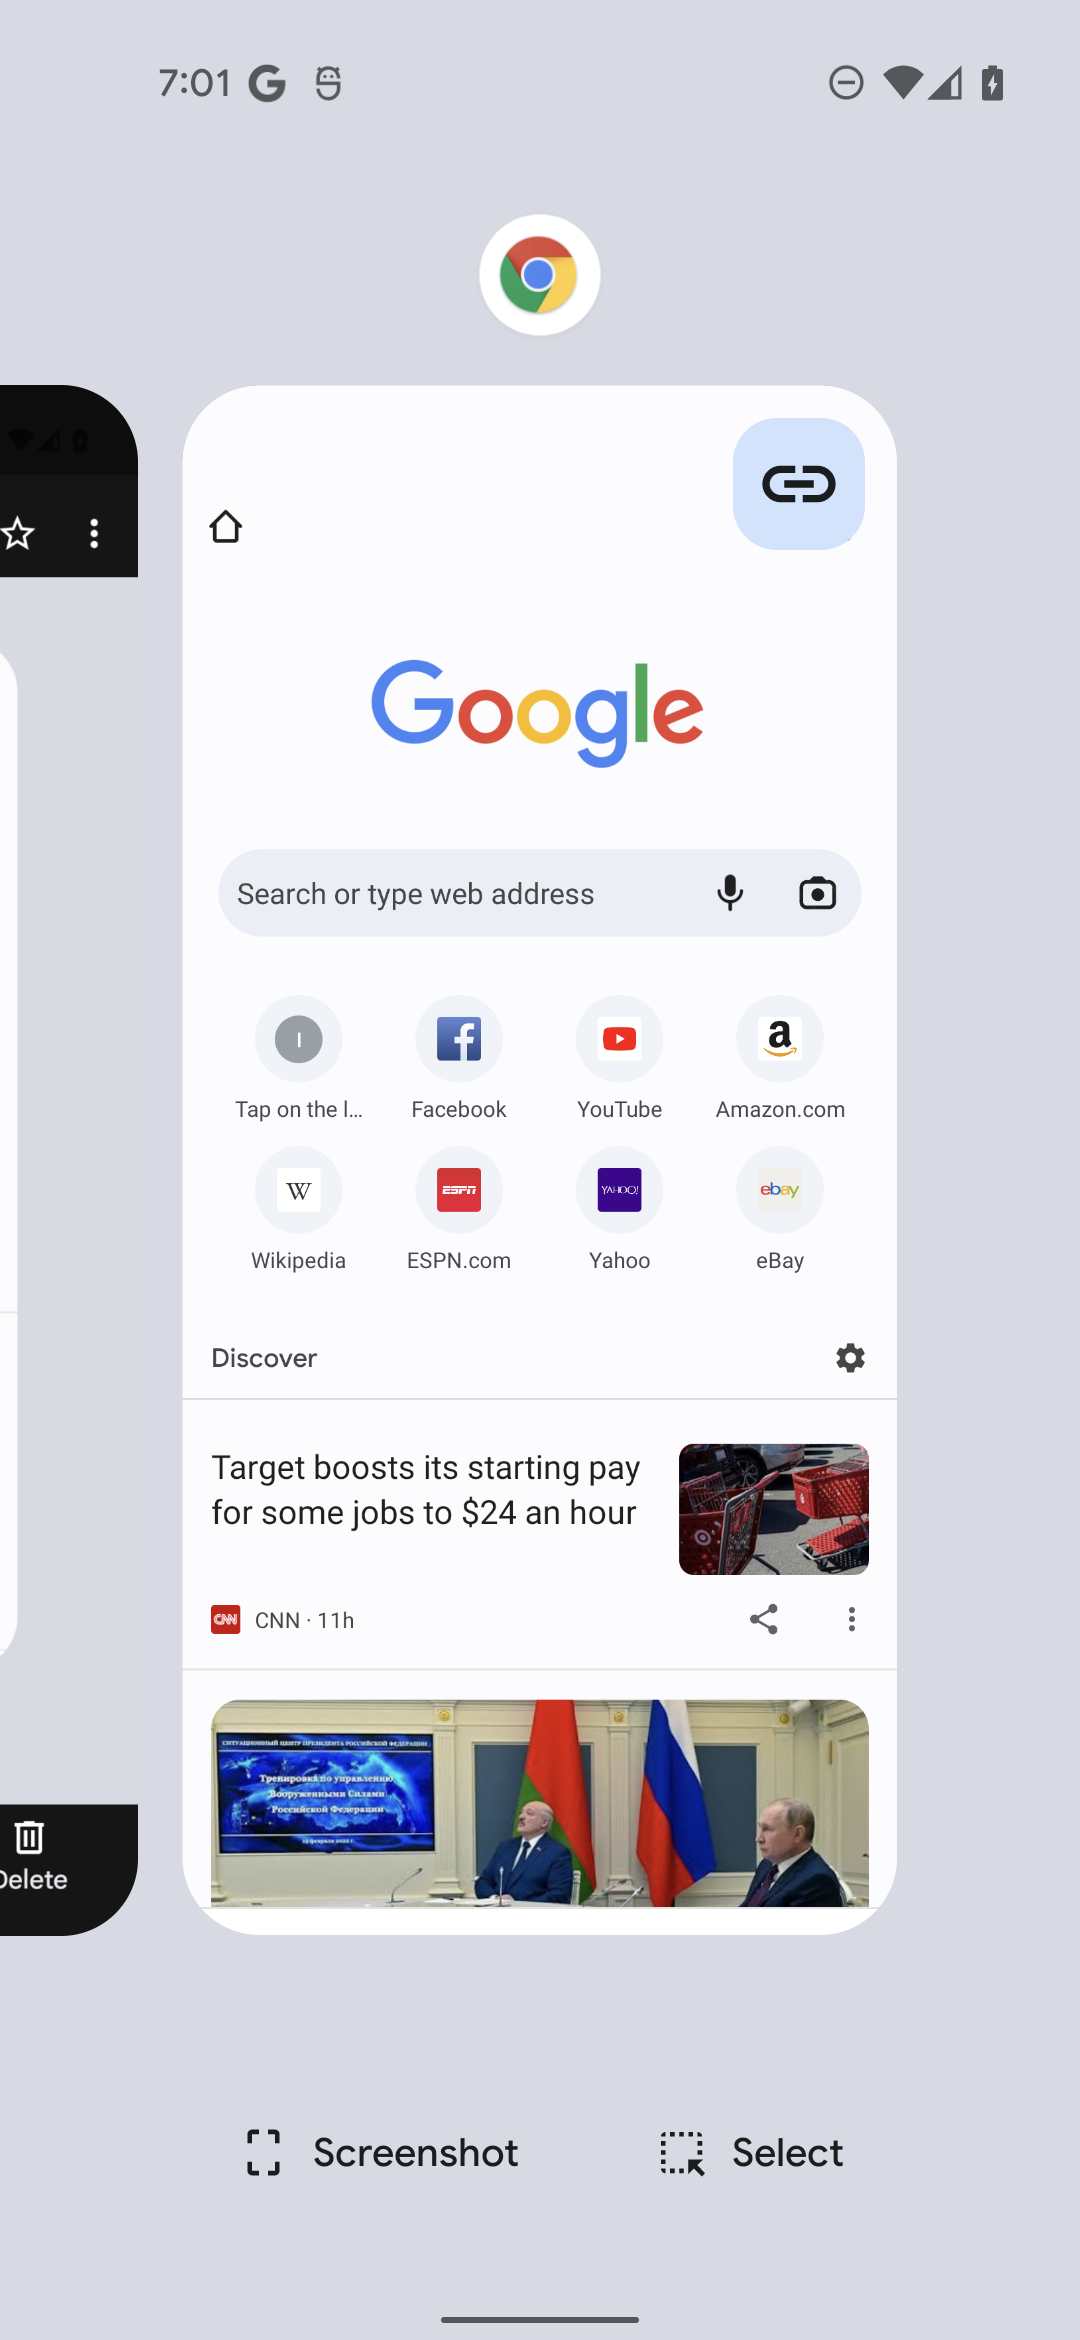
\includegraphics[width=0.8\columnwidth]{figures/recents-screen.pdf}
\caption{A screenshot of Recents screen showing that Chrome is recently accessed. However, a spyware app will not appear in the recent screen (if it chooses to hide from the recent screen), despite that one of its Activities is recently created and displayed.}
\label{fig:recents_screen}
\end{figure}


\subsubsection{Mitigations}
For apps that seek to hide their icons, our recommendation is that \DIFdelbegin \DIFdel{an app that
does not have a launcher activity should not }\DIFdelend \DIFaddbegin \DIFadd{Android should enforce stricter requirements on what apps can hide icons (e.g., the three requirements from Android 10 build r1 to r14 mentioned in footnote~\ref{footnote:hide_icon}).
Most apps that }\DIFaddend run on Android phones \DIFdelbegin \DIFdel{. If it runs,
then it should }\DIFdelend \DIFaddbegin \DIFadd{should be required to }\DIFaddend have an icon. In the case of exploiting TV app features, while we
understand that running apps with only \texttt{LEANBACK\_LAUNCHER} activities on
Android phones increases compatibility, such a feature leads to abuse as Spy24
has already demonstrated.

Launching apps by predetermined signal from another app is not only used for
malicious purposes but also for benign purposes (e.g., dial pad can be used for
testing and numerous benign apps use a browser link to open themselves).
While browser links can be easily tracked by examining the manifest, currently
users have no way to discover if apps can launch themselves with hidden codes.
The difficulty is in part because hidden codes are used dynamically during
runtime: the outgoing dialed number is sent to apps, and apps can freely decide
what actions to perform based on the number received. This design makes it hard
for the Android system to identify what hidden numbers are being tracked by each
app.  One possible mitigation is to \DIFdelbegin \DIFdel{add }\DIFdelend \DIFaddbegin \DIFadd{allow users to review apps that can receive predetermined signals (e.g., }\DIFaddend a list of apps that listen for the
\texttt{NEW\_OUTGOING\_CALL} intent or have intent filters for specific \DIFaddbegin \DIFadd{browser }\DIFaddend links,
perhaps as part of the privacy dashboard\DIFaddbegin \DIFadd{)}\DIFaddend .

One potential fix to stop apps from hiding from the Recents screen is to enforce
having at least one activity per app in the Recents screen.




\subsection{\DIFdelbegin \DIFdel{Persistency}\DIFdelend \DIFaddbegin \DIFadd{Persistence}\DIFaddend }
\DIFaddbegin \label{subsec:persistence}
\DIFaddend This section describes the methods used by spyware apps to persist on the target
device by obscuring the uninstallation process and creating ``diehard'' services
(automatically restarting \DIFdelbegin \DIFdel{them }\DIFdelend \DIFaddbegin \DIFadd{themselves }\DIFaddend after stops and reboots).

%\subsubsection{Capabilities}

\subsubsection*{Capability \#7: Obscuring the Uninstallation Process}

One way to prevent users from stopping and uninstalling an app is by
disabling the Force Stop and Uninstall buttons (see
Figure~\ref{fig:da} in the appendix).  For Android versions below 7.1,
these buttons can be disabled simply by registering the app with
\texttt{Device Administrator\DIFdelbegin \DIFdel{(DA)}\DIFdelend } \DIFaddbegin \DIFadd{(DA) }\DIFaddend privileges (as detailed \DIFdelbegin \DIFdel{by }\DIFdelend \DIFaddbegin \DIFadd{in }\DIFaddend prior
work~\cite{shan2019device}). To enable these two buttons, the user
would have to deactivate the device administrator privileges for the
app.
%
Since Android 7.1, while the Force Stop button is disabled for DA
apps, the Uninstall button will remain enabled even if the app
registers as \DIFdelbegin \DIFdel{a DAapp}\DIFdelend \DIFaddbegin \DIFadd{DA}\DIFaddend .  As a result, users can uninstall DA apps
directly~\cite{shan2019device}. Overall, we observe 11 apps that
register as DA.
%% \damon{this is really cryptic and difficult to
%% understand.}\alex{fixed}

Two apps, Cerberus and Mobile-tracker-free, directly interfere with the
uninstallation process, a behavior often observed in Android
malware~\cite{shan2019device,aljarrah2016maintaining}. Cerberus employs a series
of mechanisms to stop users from deactivating it as a DA app or
uninstalling it. These include trying to lock the device by invoking the
\texttt{lockNow} method of the \texttt{DevicePolicyManager} class and starting
an activity that blocks users from clicking on any buttons. Mobile-tracker-free,
on the other hand, tries to stop users from uninstalling it by starting an
Activity that blocks the uninstallation screen and requests a password set
by the abuser to proceed.

\subsubsection*{Capability \#8: Creating Diehard Services}
%\alex{a new title?}
%
Spyware apps strive to always be executing on the target device so
that they can collect as much information as possible.  We focus on
the ``diehard'' mechanisms that apps use to automatically restart
themselves after being stopped by the Android system \DIFaddbegin \DIFadd{(e.g., due to low memory) }\DIFaddend or after device
reboots. Echoing the diehard implementations discovered in prior
work~\cite{shao2019lightweight,zhou2020demystifying}, we observe two
main ways used by spyware apps to create diehard services. We observed
a third approach that appears to originate from the spyware ecosystem
and be a byproduct of other capabilities.

\textbf{Leveraging Scheduling Frameworks.} Scheduling frameworks such as
\texttt{JobScheduler}~\cite{JobSched94:online} and
\texttt{AlarmManager}~\cite{AlarmMan39:online} enable apps to repeatedly
restart. Apps can schedule to be restarted either when they are
first started or when they are being terminated by the system. To schedule
themselves to be restarted shortly after they are terminated, they override the
\texttt{onDestory} function, which is called before the app is terminated by the
system.

\textbf{Monitoring System Broadcasts.} Monitoring system broadcasts offers another way to wake up apps if they are not running already. Android sends broadcasts when various system events occur~\cite{Broadcas25:online}, and apps that monitor these system broadcasts will be woken up if they are not running already. Table~\ref{tab:monitor_broadcast} lists various systems broadcasts and the number of apps that monitor them.\footnote{Only a small number system broadcasts can be used to wake up apps after the restrictions introduced in Android 8~\cite{Implicit72:online}. We only consider these system broadcasts.} The spyware apps in our study predominantly use the \texttt{BOOT\_COMPLETED} broadcast. Monitoring
\texttt{BOOT\_COMPLETED} allows spyware apps to restart themselves
after the device reboots: the Android system will send a
\texttt{BOOT\_COMPLETED} system broadcast upon reboot, and spyware apps that listen
for this broadcast will automatically restart themselves. While \texttt{NEW\_OUTGOING\_CALL} \DIFdelbegin \DIFdel{is }\DIFdelend \DIFaddbegin \DIFadd{and }\texttt{\DIFadd{SMS\_RECEIVED}} \DIFadd{are }\DIFaddend also popular, we note that \DIFdelbegin \DIFdel{it serves dual-purposes (}\DIFdelend \DIFaddbegin \DIFadd{they serve dual purposes (}\texttt{\DIFadd{NEW\_OUTGOING\_CALL}} \DIFaddend can be used to launch a hidden app \DIFdelbegin \DIFdel{as well as wake an app up}\DIFdelend \DIFaddbegin \DIFadd{and }\texttt{\DIFadd{SMS\_RECEIVED}} \DIFadd{can be used to monitor SMS messages}\DIFaddend ).

\textbf{Listening for Accessibility or Notification Events.} Apps that register as an
\texttt{AccessibilityService} or
\texttt{NotificationListener- Service}
can also survive device
reboots. However, unlike the two techniques described above,
\texttt{AccessibilityService}
is less reliable because it can be
turned off by Android for battery saving reasons\DIFaddbegin \DIFadd{~\mbox{%DIFAUXCMD
\cite{AndroidA0:online,Accessib46:online}}%DIFAUXCMD
}\DIFaddend .


\begin{table}[t]
  \begin{tabular}{lr}
    System Broadcast         &\# of Apps  \\
    \midrule
    BOOT\_COMPLETED          &10          \\
    \DIFaddbeginFL \DIFaddFL{SMS\_RECEIVED            }&\DIFaddFL{9           }\\
    \DIFaddendFL NEW\_OUTGOING\_CALL      &9           \\
    \DIFaddbeginFL \DIFaddFL{PHONE\_STATE             }&\DIFaddFL{6           }\\
    \DIFaddendFL ACL\_DISCONNECTED        &1           \\
    ACL\_CONNECTED           &1           \\
    LOCKED\_BOOT\_COMPLETED  &1           \\
    \DIFaddbeginFL \DIFaddFL{WAP\_PUSH\_RECEIVED      }&\DIFaddFL{1           }\\
  \DIFaddendFL \end{tabular}
  \caption{System broadcasts and number of apps monitoring them.\label{tab:monitor_broadcast}}
%  \vspace*{-1cm}
\end{table}

\DIFaddbegin \newcommand{\partrating}{\rating{50}}

\begin{table*}[t]
	\centering
%DIF > 	\begin{tabular}{l|m{2.5cm}|m{2.5cm}|m{3.2cm}|m{2.0cm}}
	\begin{tabular}{lm{1.8cm}m{2.0cm}m{3.1cm}m{2.6cm}m{2.6cm}}
%DIF > 		\toprule
		\DIFaddFL{Spyware Apps }& \DIFaddFL{Eavesdropping Sensitive PII }& \DIFaddFL{Cross-account Request Forgery }& \DIFaddFL{Unauthenticated Access to Victim Data }& \DIFaddFL{Poor Data Retention Practices }& \DIFaddFL{Unauthenticated SMS Commands }\\
		\midrule
		\DIFaddFL{mSPY }& \partrating &  & \DIFaddFL{Images }&  &\\
		\DIFaddFL{Mobile-tracker-free }& & & \DIFaddFL{Streaming }& & \rating{100}\\
		\DIFaddFL{Clevguard }& \partrating & & \DIFaddFL{Images* }& &\\
\ltgrey 	\DIFaddFL{HoverWatch }& & & \DIFaddFL{Audio* }& &\\
\ltgrey 	\DIFaddFL{Flexispy }& \rating{100} & & \DIFaddFL{Images/Audio* }& &\\
\ltgrey		\DIFaddFL{Spyic }&  &  & \DIFaddFL{Images* }& \partrating &\\
		\DIFaddFL{Spyhuman }& & & \DIFaddFL{Images/Audio }& &\\
		\DIFaddFL{TheTruthSpy }& \rating{100} & \rating{100} & \DIFaddFL{Images/Audio }& \rating{100} &\\
		\DIFaddFL{iKeyMonitor }& & & & &\\
\ltgrey		\DIFaddFL{Cerberus }& & & \DIFaddFL{Audio* }&  & \\
\ltgrey		\DIFaddFL{Spy24 }& & & \DIFaddFL{Streaming* }& &\\
\ltgrey		\DIFaddFL{Spapp }& & & \DIFaddFL{Images/Audio/Streaming }& \partrating & \rating{100}\\
		\DIFaddFL{Meuspy }& & & \DIFaddFL{Images/Audio }& \partrating &\\
		\DIFaddFL{Highstermobile }& & & \DIFaddFL{Images }&  &\\
%DIF > \ltgrey		LetMeSpy & & & & &\\
%DIF > 		Spylive360 & & & Images/Audio & \rating{40} &\\
%DIF > 		Talklog & & & & &\\
%DIF > 		\bottomrule
	\end{tabular}
	\caption{\DIFaddFL{Systematization of commodity spyware vulnerabilities. Circles denote the severity level of the insecurity. }\protect \partrating\DIFaddFL{\ indicates at least one instance of the insecurity; }\protect \rating{100} \DIFaddFL{indicates all app functionality is insecure; * indicates URLs are temporary and expire.
		%DIF > \sumanth{Should we move None's and No's to an empty circle? or leave that field blank? Also do we want to move the unauthenticated access column to circle's? If so we might lose information (e.g if just audio vs audio and images are affected. Suggestions?)} \geoff{(1) can you reorder the columns to match the order discussed in the section? (2) no column for SMS commands? (3) my preference is for blank cells over ``None''; (4) unauthenticated: as is conveys the info better than circles}
	}}

	\label{tab:apps_spyware_vuln}
\end{table*}



\DIFaddend %% \geoff{so ``waking
%% up apps'' is just for surviving reboots?  we might want to rename}\alex{fixed.
%% techinically apps can be woken up in many ways...after being stopped. by
%% \texttt{BOOT\_COMPLETED} seems to solely used for waking up purposes}

%We also note that the old \texttt{camera} framework has an API called
%\texttt{getSupportedPreviewSizes}, which supplies a list of supported preview
%sizes\alex{not sure about camera2 framework}.

%While the API document s

\subsubsection{Mitigations}
Apps that seek to persist by registering as device administrator will
no longer be successful as users can uninstall them on most devices
running Android 7.1 or above. For apps that seek to interfere with the
uninstallation process by creating activities or locking the device,
past literature on malware defense~\cite{fernandes2016android,
  aljarrah2016maintaining} has suggested improving attack detection
and introducing system level support for detecting and reacting when
an app window is covered.
% \geoff{are there suggestions from the malware papers?}\alex{fixed}


Prior work~\cite{zhou2020demystifying} has investigated various ways
of creating diehard apps. According to the authors, the diehard
mechanisms we observe are very resilient and can only be effectively
stopped via a force stop.
%% \geoff{``the above abuses can only be effectively stopped'' --- by abuse do you
%% mean spyware activities in general, or just the methods for keeping apps
%% alive/waking up apps?}\alex{fixed}
%% However, it is unlikely that users would force stop instead of
%% uninstall a suspicious app after they have discovered it.
Additionally, the fact that many spyware apps register as device administrator
creates another layer of complication --- while apps registered as DA may be
uninstalled directly after Android 7.1, the force stop option is disabled,
making it difficult for users to stop the spyware apps (unless they uninstall
it).
However, even if apps prevent a force stop, users can still uninstall
them.
We also recommend adding a dashboard for monitoring apps that will automatically
start themselves.\footnote{We note that some Android phones (e.g., Xiaomi) have a
built-in dashboard for managing apps that can automatically start
themselves~\cite{HowtoDis42:online}.}

%\geoff{so...no mitigation then?}\alex{fixed}


% \subsection{Discussion}
% TBD


% Before diving into the actual implementation, we first detail the general
% process of building customized camera implementations. Each camera is in
% Android is a \texttt{CameraDevice} and is responsible for producing raw data
% frames~\cite{Cameraca74:online}. Apps receive these raw data frames by
% specifying an output  buffer, which for example could be a
% \texttt{SurfaceView}, \texttt{ImageReader}, \texttt{RenderScript.Allocation},
% or \texttt{TextureView}~\cite{Cameraca74:online}.

% In practice, we observed X different customized camera implementations: (1)
% through creating 1x1 pixel SurfaceView.

% To create a camera session, provide it with one or more output target buffers
% your app can write output frames to.

% The first implementation creates 1x1 pixel previews. It requires the
% \texttt{SYSTEM\_ALERT\_WINDOW} permission to draw over other apps.
% Applications


\section{SPYWARE USER DATA PROTECTION}
\label{sec:data-leak}

%\damon{at a high level we need to make it clear that we only attempted to access our own data and we should also include citations to prior news articles and industry reports that overlap with our findings.}

%% \geoff{need to describe the various infrastructure elements involved
%%   (device, accounts, servers) and lifecycle steps (when does the
%%   abuser create/setup/access an account, does the abuser download and
%%   install the spyware on the victim's device after creating an
%%   account, abuser account registration vs victim device registration
%%   to an abuser's account, high-level of how the abuser remotely
%%   controls the spyware on the victim's device).  might also go earlier
%%   in the paper for context on app implementation, but particularly
%%   needed for understanding the data protection part.}
%\sumanth{Not sure where this should go. Here in the intro?} \geoff{yes put it here for now, don't
%  worry about the flow with other parts for now}

In this section we assess \DIFaddbegin \DIFadd{how well spyware apps secure }\DIFaddend the user data \DIFdelbegin \DIFdel{security of the spyware apps
in our data set.
%DIF < 
}\DIFdelend \DIFaddbegin \DIFadd{they exfiltrate and store.
}\DIFaddend For this assessment, in addition to the victim and the abuser, we
consider a third \DIFdelbegin \DIFdel{agent: an }\DIFdelend \DIFaddbegin \DIFadd{actor: an external }\DIFaddend attacker who seeks to undermine the
security of the spyware app.  The attacker's goal is to exploit any
integrity, authorization, and authentication issues with the spyware
app to access victim data as a third party.
% that the attacker is not supposed to have access to.

%% When discussing each of the security issues below, we note further
%% assumptions about the attacker that are specific to a particular
%% issue.

%% Table~\ref{tab:apps_spyware_vuln} summarizes the threats we
%% investigated and shows which apps are susceptible to them.

We start by describing our
\DIFdelbegin \DIFdel{overall
}\DIFdelend methodology for investigating the data protection practices of the
spyware apps, and then discuss \DIFdelbegin \DIFdel{our results for }\DIFdelend each of the \DIFdelbegin \DIFdel{threats in detail}\DIFdelend \DIFaddbegin \DIFadd{vulnerabilities we uncovered (summarized in Table~\ref{tab:apps_spyware_vuln})}\DIFaddend .

%DIF < % We focus on vulnerabilities that leave user data unprotected and
%DIF < % subject to cross-account attacks. Our methods provide a clear road map
%DIF < % for discovering security vulnerabilities in other spyware apps.
\DIFdelbegin %DIFDELCMD < 

%DIFDELCMD < %%%
%DIF <  The target device is an Android phone used by the victim. The abuser who wants to monitor the victim, first creates an account on the spyware web portal interface and purchases a subscription if required. The abuser then requires physical access to the victim's device, to download and install the spyware client app. The app configures the necessary permissions and allows the abuser to sign in (typically using the same credentials used by the web portal). The app exfiltrates data to its servers once sign in is successful. The abuser can now view the data by logging into their account on the spyware web portal, which fetches and displays data from its servers. Once logged in, the app continues to regularly sync data with its servers. Some spyware also allows abusers to perform remote actions like covertly recording audio and video, taking app screenshots, which are done on-request and uploaded to the servers. \sumanth{We might want to merge this with the Overall threat model below.}
%DIFDELCMD < 

%DIFDELCMD < %%%
%DIF < \begin{figure*}[h]
%DIF < 	\includegraphics[width=\textwidth]{figures/app_systematization_vulnerabilities.jpg}
%DIF < 	\caption{Systematization of commodity spyware vulnerabilities (Alo: At Least One occurrence, * : Public server URI not static and expires)\sumanth{Change this to a circle-format like in sam's report}]}
%DIF < 	\label{tab:apps_spyware_vuln}
%DIF < \end{figure*}
%DIFDELCMD < 

%DIFDELCMD < \newcommand{\partrating}{\rating{50}}
%DIFDELCMD < 

%DIFDELCMD < \begin{table*}[t]
%DIFDELCMD < 	\centering
%DIFDELCMD < %%%
%DIF < 	\begin{tabular}{l|m{2.5cm}|m{2.5cm}|m{3.2cm}|m{2.0cm}}
	%DIFDELCMD < \begin{tabular}{lm{1.8cm}m{2.0cm}m{3.1cm}m{2.6cm}m{2.6cm}}
%DIFDELCMD < %%%
%DIF < 		\toprule
		\DIFdelFL{Spyware Apps }%DIFDELCMD < & %%%
\DIFdelFL{Eavesdropping Sensitive PII }%DIFDELCMD < & %%%
\DIFdelFL{Cross-account Request Forgery }%DIFDELCMD < & %%%
\DIFdelFL{Unauthenticated Access to Victim Data }%DIFDELCMD < & %%%
\DIFdelFL{Poor Data Retention Practices }%DIFDELCMD < & %%%
\DIFdelFL{Unauthenticated SMS Commands }%DIFDELCMD < \\
%DIFDELCMD < 		\midrule
%DIFDELCMD < 		%%%
\DIFdelFL{mSPY }%DIFDELCMD < & \partrating &  & %%%
\DIFdelFL{Images }%DIFDELCMD < &  &\\
%DIFDELCMD < 		%%%
\DIFdelFL{Mobile-tracker-free }%DIFDELCMD < & & & %%%
\DIFdelFL{Streaming }%DIFDELCMD < & & \rating{100}\\
%DIFDELCMD < 		%%%
\DIFdelFL{Clevguard }%DIFDELCMD < & \partrating & & %%%
\DIFdelFL{Images* }%DIFDELCMD < & &\\
%DIFDELCMD < \ltgrey 	%%%
\DIFdelFL{HoverWatch }%DIFDELCMD < & & & %%%
\DIFdelFL{Audio* }%DIFDELCMD < & &\\	
%DIFDELCMD < \ltgrey 	%%%
\DIFdelFL{Flexispy }%DIFDELCMD < & \rating{100} & & %%%
\DIFdelFL{Images/Audio* }%DIFDELCMD < & &\\
%DIFDELCMD < \ltgrey		%%%
\DIFdelFL{Spyic }%DIFDELCMD < &  &  & %%%
\DIFdelFL{Images* }%DIFDELCMD < & \partrating &\\
%DIFDELCMD < 		%%%
\DIFdelFL{Spyhuman }%DIFDELCMD < & & & %%%
\DIFdelFL{Images/Audio }%DIFDELCMD < & &\\
%DIFDELCMD < 		%%%
\DIFdelFL{TheTruthSpy }%DIFDELCMD < & \rating{100} & \rating{100} & %%%
\DIFdelFL{Images/Audio }%DIFDELCMD < & \rating{100} &\\
%DIFDELCMD < 		%%%
\DIFdelFL{iKeyMonitor }%DIFDELCMD < & & & & &\\		
%DIFDELCMD < \ltgrey		%%%
\DIFdelFL{Cerberus }%DIFDELCMD < & & & %%%
\DIFdelFL{Audio* }%DIFDELCMD < &  & \\
%DIFDELCMD < \ltgrey		%%%
\DIFdelFL{Spy24 }%DIFDELCMD < & & & %%%
\DIFdelFL{Streaming* }%DIFDELCMD < & &\\
%DIFDELCMD < \ltgrey		%%%
\DIFdelFL{Spapp }%DIFDELCMD < & & & %%%
\DIFdelFL{Images/Audio/Streaming }%DIFDELCMD < & \partrating & \rating{100}\\
%DIFDELCMD < 		%%%
\DIFdelFL{Meuspy }%DIFDELCMD < & & & %%%
\DIFdelFL{Images/Audio }%DIFDELCMD < & \partrating &\\
%DIFDELCMD < 		%%%
\DIFdelFL{Highstermobile }%DIFDELCMD < & & & %%%
\DIFdelFL{Images }%DIFDELCMD < &  &\\
%DIFDELCMD < %%%
%DIF < \ltgrey		LetMeSpy & & & & &\\
%DIF < 		Spylive360 & & & Images/Audio & \rating{40} &\\
%DIF < 		Talklog & & & & &\\
%DIF < 		\bottomrule
	%DIFDELCMD < \end{tabular}
%DIFDELCMD < 	%%%
%DIFDELCMD < \caption{%
{%DIFAUXCMD
\DIFdelFL{Systematization of commodity spyware vulnerabilities. Circles denote the severity level of the insecurity. }%DIFDELCMD < \protect \partrating%%%
\DIFdelFL{\ indicates at least one instance of the insecurity; }%DIFDELCMD < \protect \rating{100} %%%
\DIFdelFL{indicates all app functionality is insecure; * indicates URLs are temporary and expire. 
		%DIF < \sumanth{Should we move None's and No's to an empty circle? or leave that field blank? Also do we want to move the unauthenticated access column to circle's? If so we might lose information (e.g if just audio vs audio and images are affected. Suggestions?)} \geoff{(1) can you reorder the columns to match the order discussed in the section? (2) no column for SMS commands? (3) my preference is for blank cells over ``None''; (4) unauthenticated: as is conveys the info better than circles}
	}}
%DIFAUXCMD
%DIFDELCMD < 

%DIFDELCMD < 	\label{tab:apps_spyware_vuln}
%DIFDELCMD < \end{table*}
%DIFDELCMD < 

%DIFDELCMD < %%%
%DIF < \sumanth{TODO: Re-write table}
%DIFDELCMD < 

%DIFDELCMD < %%%
%DIF < \subsection{Overall Threat Model}
%DIFDELCMD < 

%DIFDELCMD < %%%
%DIF < % \geoff{with the context from Section 2.1, we can trim this down just
%DIF < %   to focus on introducing the attacker}\sumanth{Trimmed.}
%DIFDELCMD < 

%DIFDELCMD < %%%
%DIF < For each spyware app, we consider three agents: a victim, an abuser
%DIF < who targets and monitors the victim, and an attacker who seeks to
%DIF < undermine the security of the spyware app.  The abuser, having
%DIF < procured a spyware subscription, installs the spyware app on a
%DIF <  victim's device, and logs in with their credentials. The abuser's
%DIF < goal is to surreptitiously monitor the victim using the spyware app on
%DIF < the victim's device.
%DIFDELCMD < 

%DIFDELCMD < %%%
%DIF < % Within each insecurity listed below,
%DIF < % we further note all the assumptions the attacker must learn to
%DIFDELCMD < 

%DIFDELCMD < %%%
%DIF < % For each spyware app, we consider three agents: a victim whose is to be monitored, an abuser who is targeting the particular victim, and an attacker who is seeking to undermine the security of the spyware app. The abuser (having procured a spyware subscription) installs spyware on a victim's device, and logs in with the app credentials. The abuser's goal is to surreptitiously monitor the victim through the device infected with the spyware. The attacker's primary goal is to exploit the integrity, authorization, and authentication issues with a spyware application in order to uncover user data that the attacker is not supposed to have access to. Within each insecurity listed below, we further note all the assumptions the attacker must learn to
%DIFDELCMD < 

%DIFDELCMD < %%%
%DIF < % \geoff{we should explicitly describe the overall scenario: abuser has
%DIF < %   installed spyware on a victim's device, and a third-person attacker
%DIF < %   wants to gain access to victim data the spyware has collected, or
%DIF < %   control the spyware.  need to work out what we assume about
%DIF < %   attackers here vs in each individual subsection below.} \sumanth{I've explained the overall scenario here. I believe we don't need to assume anything here, and the per-insecurity threat models are fairly detailed in their assumptions.}
%DIFDELCMD < 

%DIFDELCMD < %%%
\DIFdelend \subsection{Methodology}
\label{subsec:experiemental_setup}

%\sumanth{Revised methodology section 4.1}
For each app we analyzed, we obtained an account (providing payment
information when necessary) and registered the app on a Pixel 2 XL
Android phone running Android 10.
%% We used man-in-the-middle (MITM) traffic inspection to perform our
%% network analysis on each spyware app.

To identify apps sending data \DIFdelbegin \DIFdel{via unencrypted HTTP we used tcpdump}\DIFdelend \DIFaddbegin \DIFadd{from the device to the backend servers via unencrypted connections we used }\texttt{\DIFadd{tcpdump}}\DIFaddend ,
listening on a Windows 10 machine interface configured as a mobile
hotspot, to capture and inspect app traffic over the network.  We
configured the Android phone to connect to the PC and recorded all
traffic exchanged with the app servers, without any proxy in between
(avoiding any potential TLS handshake failures due to certificate
pinning).

To study the interactions between the spyware web portal interface and
the spyware backend servers, we used the open-source \DIFdelbegin \DIFdel{MITMProxy }\DIFdelend \DIFaddbegin \texttt{\DIFadd{MITMProxy}} \DIFaddend tool to
decrypt HTTPS traffic.  This configuration gave us access to
authentication tokens (session cookies, secrets, etc.) for conducting
forgery attacks on our test accounts.  We were able to login to all
portals without error (e.g., there were no issues with certificate
pinning).  We also analyzed the HTML content displayed via the spyware
web portal interface, extracting the URLs linked to uploaded user
media (images, audio, etc.).  We then performed a sequence of
experiments that tested and verified each insecurity listed in
Table~\ref{tab:apps_spyware_vuln}.

% we installed a trusted PEM certificate (generated
% by the proxy) on the phone, adding the certificate to the list of user
% store certificate authorities.

%% \geoff{could also aggregate the specific methodology parts from the
%%   subsections here}

%% For each app we analyzed, we obtained an account (providing payment information when necessary) and registered the app on a Pixel 2 XL Android phone running Android 10. We used a man-in-the-middle (MITM) traffic inspection approach to perform our network analysis on each spyware app, focusing on outgoing requests from each app that we manually installed on the Android phone. We leveraged the open-source MITMProxy tool to inspect outgoing requests, which we setup and ran on a Windows 10 PC noting its IP address. We then configured the Android phone to connect to a mobile hotspot setup on the PC, and configured a manual proxy to route all traffic to port 8080 - that the traffic inspector actively ran on. In order to decrypt TLS traffic, we installed a trusted PEM certificate (generated by the traffic inspector) on the phone, which adds the certificate to the list of user store certificate authorities. For each spyware app, we installed the mobile app onto the Android phone, logged in using the abusers credentials and ran through the sequence of experiments which test each insecurity listed in table \ref{tab:apps_spyware_vuln}.
%% We also analyzed the spyware web portal interface and extracted the path for uploaded user media (images, audio, etc) which we used for the following experiments.

\subsection{Results}

Table~\ref{tab:apps_spyware_vuln} summarizes the threats we
investigated and shows which apps are susceptible to them.
%
We describe each of the threats in turn, summarizing its context, its
associated threat model, any additional methods we employed, and the
specific results we discovered for the vulnerable apps.

%% We start by briefly describing each insecurity, along with the threat
%% model and experimental setup used to identify the insecurity. We then
%% discuss a subset of the apps which demonstrate each insecurity. To
%% structure our analysis, we focused on security mechanisms for
%% protecting sensitive user data.

%We are less interested in flows that do not aid in compromising the app or user data; for example, apps that are using unsecured HTTP connections for non-sensitive functionality.

%% \geoff{the structure of these subsections results in some redundancy
%%   across the various parts, which is not ideal.  but it does have the
%%   virtue of being explicit about each of the parts.}

%\subsubsection*{Insecurity \#1: Submitting sensitive victim or abuser PII over the network}
\subsubsection*{Insecurity \#1: Eavesdropping sensitive \DIFaddbegin \DIFadd{personally identifiable information (}\DIFaddend PII\DIFaddbegin \DIFadd{)}\DIFaddend }
%\subsubsection{Eavesdropping sensitive PII}

Some spyware apps transmit highly sensitive victim data, such as photos,
texts, and location, from the victim device to the spyware backend
servers using unencrypted HTTP connections.  A MITM attacker who
eavesdrops on the same communication channel (e.g., same WiFi network)
\DIFdelbegin \DIFdel{would be able to }\DIFdelend \DIFaddbegin \DIFadd{could }\DIFaddend collect all data and credentials sent unencrypted
over the network.  \DIFdelbegin \DIFdel{Further}\DIFdelend \DIFaddbegin \DIFadd{Furthermore}\DIFaddend , credentials leaked over the network enable
an attacker to login to the abuser's account and gain access to all of
the victim's data exfiltrated by the spyware.

\textbf{Threat model.} We assume that the attacker can eavesdrop on
all messages sent by the mobile device infected with spyware (e.g.,
the attacker uses the same WiFi network as the victim, and the WiFi
network is not using link-layer encryption).

%% We also assume that the network used when eavesdropping is unencrypted
%% (e.g., a WiFi network not using link-layer encryption).

%% \geoff{doesn't the WiFi network need to
%%   be unencrypted (not use link-layer encryption)?} \sumanth{Addressed}

\textbf{Experimental setup.}
%% To uncover sensitive data flows, we utilized the spyware's
%% functionality and observed the outgoing network traffic from the
%% target device.
We filtered the captured traffic to observe network activity from \DIFdelbegin \DIFdel{the apps }\DIFdelend \DIFaddbegin \DIFadd{each app }\DIFaddend over
insecure channels like HTTP, and used a combination of search and
manual inspection to analyze the recorded traffic for sensitive data
such as leaked credentials (user names, email addresses, passwords),
text messages, call logs, etc.

%% Filter's were setup to flag any network activity over insecure
%% channels like HTTP. These packets were manually analyzed to see if
%% they leaked passwords, messages, call logs, etc. Similarly we flagged
%% packets containing sensitive PII's (i.e., user/abuser email) using
%% regex matching.

%% \damon{did we check for password, sms, call logs, messages?}
%% \sumanth{Added a line above that we analyzed insecure packets to see
%%   if they leaked all these.}

\textbf{Results.}  Four spyware apps in our study leak at least some
of their data using vulnerable communication channels.  TheTruthSpy
submits all of its data over HTTP, and it leaks the abuser's
credentials for TheTruthSpy servers (abuser email address and
password) in the authentication request during app setup.
%% It also leaks the abuser email address
%% in response to an unauthenticated request for registration information.
%% TheTruthSpy also leaks the abuser's email address in the response to
%% an endpoint called during setup time.
%% \geoff{victim's?}
%% \sumanth{Edited to make it clearer. There are 2 cases - email and pwd
%%   leaked in a request during setup time, and just the email leaked in
%%   the response every time a particular endpoint is called}.
%% \geoff{``endpoint'' is still a bit vague? if the email address leak is
%%   also during setup, then I think we can leave it out (the full
%%   credential leak is already a worse case)}
mSPY leaks only
the upload path for its images in an HTTP response back to the
victim's device when the image upload succeeds.
%\sumanth{Added this for Clevguard}
Clevguard uploads its images over HTTP, making it is possible for an attacker to reconstruct the image from the payload.  Flexispy uses
HTTP for all of its communication, but it implements a custom
encryption protocol for the data it sends.  However, a previously
discovered flaw in Flexispy's encryption makes it possible to
intercept personal data sent over the
network~\cite{Stalking85:online}.

%% We observed 3 spyware apps send their data - like texts, images,
%% locations - over plain HTTP protocol. \textbf{TheTruthSpy} submits all
%% its data over HTTP. Further, it leaks both the abuser email and
%% password during app setup time (when authenticating), and the abuser's
%% email during setup time. \textbf{mSpy} on the other hand leaks only
%% the upload path for its images in a HTTP response back to the victim's
%% device once the upload is successful. While both these apps send data
%% in the clear, \textbf{Flexispy} implements a custom encryption
%% protocol even though it sends data over HTTP. However, a perviously
%% discovered flaw in Flexispy's encryption makes it possible to
%% intercept personal data being sent over the network
%% \cite{Stalking85:online}.

\subsubsection*{Insecurity \#2: Cross-account request forgery}
%\subsubsection{Cross-account request forgery}

Knowing a particular user identifier, or \DIFdelbegin \DIFdel{having access to }\DIFdelend a file path \DIFaddbegin \DIFadd{that provides access }\DIFaddend to images, audio, or video on the server, an attacker can use valid
cookies from one spyware account to access data or perform actions in
the accounts of other spyware users.

\textbf{Threat Model.} The attacker can register a spyware account and
log into it. Using a MITM traffic inspector (similar to our proxy
described in Section~\ref{subsec:experiemental_setup}), an attacker
can intercept and replay authenticated requests from their account. We
assume the attacker knows the ID of the targeted user's account ---
either through enumeration, or from the ID being leaked over the
network or in a public data dump~\cite{mSpybrea38:online,
  Companyt8:online, HackerSt66:online, Cerberus12:online,
  Stalkerw59:online}.

%% \damon{this is cryptic, I would suggest directly stating that the
%%   attacker can register/purchase a spyware account and log into it.}
%% \geoff{still cryptic :-) \sumanth{Reworked this section. Hope its
%%     better now :)}}

\textbf{Experimental setup.} We used two accounts for each app, one
for the attacker and the other as the targeted spyware user.  We then
recorded and replayed authenticated requests from the attacker's
account to the targeted user's account, substituting the ID of the
targeted user's account in the requests without changing authorization
tokens provided by the attacker's account (e.g., session IDs, API
keys).  We only replayed requests to our test accounts, and
made no attempt to access content belonging to any other account.

%% \sumanth{Reworked based on Damon's feedback}\damon{this need to be
%%   improved to better describe that we had two accounts and that we
%%   checked for cross-account data leakage. We should also be clear that
%%   we only probed our own accounts and we did not attempt to access any
%%   content that potentially belonged to another person's account.}

\textbf{Results.}  Only one of the apps in our study is vulnerable to
cross-account request forgery.
%% We disregarded apps which have API
%% structures with no IDs that identify users or devices, and instead
%% rely solely on session IDs for authentication and
%% identification.
%% \sumanth{Added this to tie well with results in table}
%% \geoff{I'm still not sure the distinction between ``No'' and ``--'' in
%%   the table.  does ``--'' mean that by design the app is not
%%   suscectiple to CARF?  and No means that the app's design could be
%%   susceptiple but its implementation is correct?} \sumanth{Yes, exactly!}
With TheTruthSpy, it was possible to
access all data (messages, contacts, locations, images, etc.)  in the
targeted account using a cookie provided by the attacker's account,
and simply swapping the attacker's device ID with the targeted
account's device ID in requests to TheTruthSpy server.  Furthermore,
when we registered multiple test accounts in succession, we noticed
that the device ID \DIFdelbegin \DIFdel{the }\DIFdelend \DIFaddbegin \DIFadd{that }\DIFaddend TheTruthSpy assigns to a new device is a six-digit
integer which increases incrementally when new devices are registered.
%% \damon{how did we determine that it increased
%%   incrementally?}\sumanth{I see newer accounts always get assigned
%%   higher numbers which are very close by to older ones. I tested with
%%   2 accounts and found the deviceIDs were close by.}
The combination of insecure access controls across accounts and
predictable device IDs makes it possible for an attacker to retrieve
data from other accounts without needing to identify the device ID
beforehand.

%% by swapping the
%% device ID of a target account, while using valid cookies provided by
%% the first account. Furthermore, the device ID TheTruthSpy assigns to a
%% new device is a 6 digit integer which increases incrementally when new
%% devices are registered. \damon{how did we determine that it increased
%%   incrementally?}\sumanth{I see newer accounts always get assigned
%%   higher numbers which are very close by to older ones. I tested with
%%   2 accounts and found the deviceIDs were close by.} The combination
%% of insecure access controls across accounts and predictable device ID
%% makes it possible for an attacker to retrieve data from other accounts
%% without needed to know the device ID beforehand.

% \sumanth{TODO: Any other CARF in other apps?}

%\subsubsection*{Insecurity \#3: Leaking sensitive data on public server URIs}
\subsubsection*{Insecurity \#3: Unauthenticated access to victim data}
%\subsubsection{Unauthenticated access to victim data}
\label{sec:leaky-urls}

%% \geoff{would be good to describe the scenario: some apps use CDNs or
%%   backend servers to store media data (do we know why? cost?), and the
%%   URLs they generate to the media data are unauthenticated.  the idea
%%   is to note the distinction between URLs to content on the app's server
%%   vs URLs to media stored on different infrastructure (which is my
%%   understanding of what's going on here, which may be wrong?)  either
%%   way, we want to give some sense/intuition for why URLs for accessing
%%   this content is different than other content stored on the spyware
%%   servers.} \sumanth{Good point! I've added this in the intro of the section below. One thing missing might be the reasoning as to why they choose to store media on different servers. Cost might be the main reason yes.)} \geoff{thanks, edited}

Many of the spyware apps use different backend infrastructure \DIFdelbegin \DIFdel{,
separate from the server infrastructure serving spyware account
access, }\DIFdelend to store
and deliver media data \DIFdelbegin \DIFdel{.  }\DIFdelend \DIFaddbegin \DIFadd{that is distinct from the servers that
abusers use to access the app dashboard (e.g., abusers login
to the dashboard via the website domain in Table~\ref{tab:apps_selected}, but
the app may use a CDN to deliver images and videos).
}\DIFaddend This separate infrastructure
includes cloud storage (e.g., AWS S3 buckets), content distribution
networks, and other shared hosting services, all of which are
presumably cheaper to use for serving media data.  We observed that
some of the spyware apps are \DIFdelbegin \DIFdel{much }\DIFdelend less careful about protecting the
data that they store on \DIFdelbegin \DIFdel{the shared }\DIFdelend \DIFaddbegin \DIFadd{this hosting }\DIFaddend infrastructure, often allowing
unauthenticated access to the URLs they generate to stored media data.
Further, we observed user data stored in predictable URLs that make it
possible to access data across different accounts, protected solely
through security by obscurity and vulnerable to enumeration. Table~\ref{tab:apps_spyware_vuln} lists
the kinds of data leaked in public URLs for the apps studied. Failure
to authenticate access to user media (like images, audio, etc.) using
mechanisms like cookies is a common example of this category of
vulnerability.

\textbf{Threat model.} We assume that the attacker has knowledge of
the media upload path for the app based on studying media paths
revealed using accounts owned by the attacker.  For apps that use the
device ID in URL path components, we also assume the attacker knows
the targeted device ID.

\textbf{Experimental setup.} To discover sensitive data leakage, we
focused primarily on URLs used to store media artifacts (images,
audio, video, etc.).  We extracted these URLs by examining the
browser-generated HTML content when accessing the dashboard in the
spyware account.  We only attempted to access media upload paths from
our test accounts, and made no attempt to access content belonging to
any other account.

%% \geoff{how did you collect URIs using the attacker's account?}
%% \sumanth{Addressed. Also added another statement to make sure we are
%%   clear that we collected media links from our own accounts}

\textbf{Results.}  Six of the apps in our study store their data in
public URLs accessible without authenticated access.  We disregarded
apps which store data in URLs that, although public, expire after a
short duration (e.g., Spyic's links to images expire after 1,800
seconds).

% We also disregard those apps which required authenticated
%(cookie-based) access to data. \geoff{not sure the distinction between
%  this case and other authenticated account access?}

Highstermobile stores its images with a URL scheme as a concatenation
of the image upload timestamp (UNIX timestamp with seconds precision)
and a double digit random number, with no other per-device ID in the
path (e.g.,
\texttt{\url{https://domain.com/path/photo_<timestamp><00-99>.png}}).
% \sumanth{\url{https://evt17.com/iphone/uploads/gallery/image/thumb/photo_<UNIXTimestamp><00-99>.png}}.
Since an attacker could plausibly iterate over a short range of
timestamps and random digits, this naming scheme makes it
straightforward for an attacker to gain unauthorized access to media
stored on the server for other accounts.

Cerberus and Spyhuman use public URLs that are a combination of device
ID and Unix timestamp
% (also Unix timestamp with seconds precision)
(e.g., \texttt{\url{https://domain.com/<DeviceID>-<timestamp>.ext}}).
While both of them require the attacker to know the device ID before
hand, an attacker could for instance obtain the device ID from data
dumps made public in breach attacks~\cite{mSpybrea38:online,
  Companyt8:online, HackerSt66:online, Cerberus12:online,
  Stalkerw59:online} or with physical access to the device.
%% \geoff{I added this, are there better scenarios?} \sumanth{Maybe also
%%   from public data dumps which have device metadata?}
Cerberus stores audio insecurely using the device IMEI as the device
ID.  Spyhuman stores both its images and audio insecurely using the
Android serial number as its device ID.  With both apps, an attacker
knowing the device ID could plausibly iterate over a short range of
timestamps to retrieve data stored on the server.

% \url{https://www.cerberusapp.com/audio/<DeviceID>-<UNIXTimestamp>.mp4}
% \url{https://dwnlnew.webdown2.com/rec/<DeviceID>/<UNIXTimestamp>/file.mp3}

Three other apps store data on servers using public URLs that rely on
security through obscurity, but they generate URLs that are neither
enumerable or predictable.  For instance, Spy24 allows WebRTC remote
streaming through a public URL based on a request ID generated by the
app, Spapp requires two alphanumeric keys to access image and audio
files on the server, and Meuspy generates unguessable URLs to
store images and audio.  Although certainly not good security
practice, the risk associated with unauthenticated access is lower
than for the other apps we discussed.

%% these three apps do not implement
%% good security practice by solely depending on security by obscurity,

%% \geoff{conclusion?  not good security
%%   practice but lower risk than the other apps?} \sumanth{Added.}

% complicated

%% Among the other 3 apps which leaked data on public server, all of them generate URIs which although public, is neither enumerable or predictable. These rely solely on Security through obscurity. \sumanth{e.g \textbf{Spy24.app} (which allows WebRTC remote streaming through a public URL based on a request ID generated by the app), \textbf{Spapp} (which requires 2 alphanumeric keys to access any image/audio on the server) and \textbf{Spylive360} (which generates complicated URLs to store images/audio)}

\subsubsection*{Insecurity \#4: Poor data retention practices}
%\subsubsection{Poor data retention practices}

%% \sumanth{I rewrote this section to better explain what I had in mind.}

Some spyware apps have poor data retention practices that prevent
victim data from being deleted from the spyware servers. %DIF < % , in some cases because the data is either unaccessible by the abuser
%DIF < % or unassociated with any account.
These data retention issues pose \DIFdelbegin \DIFdel{a risk if a data breach exposes
}\DIFdelend \DIFaddbegin \DIFadd{serious security and privacy risks~\mbox{%DIFAUXCMD
\cite{santhanam2022scraping}}%DIFAUXCMD
. A data breach could expose }\DIFaddend residual victim PII which has persisted even if, for instance, the abuser has deleted their account.

%DIF > % , in some cases because the data is either unaccessible by the abuser
%DIF > % or unassociated with any account.
\DIFaddbegin 



\DIFaddend %% All there of these cases involve unauthorized transmission of data which remains on the server indefinitely, and is either unaccessible by the abuser or unassociated with any account. These scenarios poses a risk if a data-breach exposes residual victim/attacker PII which has continued to persist.

%% \geoff{if we just have one app that has all of these risks, then we'll
%%   want to rework the story a bit}

%% Again, all data uploaded in both of these cases has the potential to
%% be leaked in a data breach.

%% \sumanth{I rewrote this section to better explain what I had in mind. Broadly speaking there are 3 cases here - Unassociated data sent without logging in, data sent but inaccessible without purchase, data sent after license expires or app is deleted. I've moved the part of 'delete' not actually deleting data to the end of section 4 along with the other misc stuff.}

%\geoff{who installed the app but never
%  used it?  an abuser who decided not to use it?  is this a compelling
%  risk?}

%% \geoff{do the apps provide the capability for the abuser to delete
%%   uploaded victim data via their server account?  if so, did we test
%%   to see if that data is actually deleted?  if not, there might not be
%%   time to do it for the submission, but is something to add for later} \sumanth{Yes, for apps which allowed the delete account option, I tried to see if both uploaded media and replaying endpoints to get, and have results for this}

%% Some apps send user data (like text messages, images, keylogger activity) to the spyware app servers before the abuser logs in/sets up the account. In some cases, this data is never visible to the attacker but is stored on the server. In some cases, user data (like images, audios, text messages, etc) persists even after explicitly deleting the account associated with the abuser. Further, in the event the license expires some spyware apps continue to send data to the backend servers, unaware of the expired license. This poses a particular issue if a data-breach exposes sensitive user data of victim's, who might have installed but never used the app \cite{esetandr4:online}

\textbf{Threat model.} Data uploaded to the spyware servers and never deleted poses a long-term risk to being made public in data dumps associated with breach attacks.
%\sumanth{I'm not sure if this has a threat model because this doesn't have an attacker per say.}
% \geoff{data never deleted poses long-term risk to data breaches?} \sumanth{Added.}

\textbf{Experimental setup.}  To \DIFdelbegin \DIFdel{see if an app was uploading data not
associated with any account, we captured network traffic from the
target device before logging in to the app for the first time.
Similarly, we }\DIFdelend \DIFaddbegin \DIFadd{discover poor data retention practices, we }\DIFaddend analyzed network traffic generated after the \DIFaddbegin \DIFadd{app }\DIFaddend license expired, but \DIFdelbegin \DIFdel{left }\DIFdelend \DIFaddbegin \DIFadd{with }\DIFaddend the victim device still logged in.  We also tested
access to media on deleted accounts using their public URLs up to
seven days after deletion of the account.
%\sumanth{Added this line.}

%% Network traffic from the target device was captured and analyzed
%% before the abuser logged in and after the license expired.  Data
%% uploaded to the server was tested for persistence after the account
%% was expired.

\textbf{Results.}  Four of the apps in our study demonstrate poor data retention practices.

Consistent with its other data vulnerabilities,
TheTruthSpy also has data retention issues.
% \sumanth{Based off of reviewer C's comments, I omitted the data sent before registration result here. We now only talk about the data sent after license expiry and data retained after account deletion.}
It continues to send
data from the victim's phone (e.g., text messages, images, keylogger
activity) to its servers after the app license expires. Further, it persists some data after the abuser
deletes their spyware portal account and the data associated with it.
%
%before the abuser even sets up their account.
%The exfiltrated data is never associated with an account and thus
%cannot be deleted even after logging in to the spyware portal.
%
%% \geoff{how is the exfiltrated data associated with the account if it
%%   is sent before the account is set up?} \sumanth{Clarified}
%% \geoff{who installed the app but never used it?  an abuser who decided
%%   not to use it?  is this a compelling risk?}
%It also continues to exfiltrate data to its servers after the app license expires.
In particular, images uploaded from the victim device persist after
account deletion, and the images remained accessible through the
public URLs used to access them (Section~\ref{sec:leaky-urls}).

%% abuser does not uninstall the logged-in app \sumanth{This seems like a
%%   common scenario abusers might do} \geoff{it does.  have we
%%   systematically tested what happens across the apps when we delete
%%   the portal account but leave the app on the device?} \sumanth{TLDR - I did capture traffic for this scenario, but the results are fuzzy, so we can omit this.}

%% Similarly, the exfiltrated data continues to be uploaded even after the abuser deletes their account, but does not uninstall the logged-in app \sumanth{This seems like a common scenario abusers  might do} or even in case the app license expires. The uploaded data, even though valid, is no longer accessible by the abuser.

Spyic has a data retention issue resulting from its trial usage
model.  When installed for trial use, Spyic uploads data from the
victim device to the server.  But it only allows access to its portal
after the abuser has purchased a subscription.  If the abuser decides
not to purchase the spyware, victim data persists indefinitely on
Spyic's servers (presumably in anticipation of the spyware user
eventually deciding to pay for a license).

%% \geoff{I added this statement, is it accurate?  do we think that
%%   Spyzie will retain the data indefinitely in anticipation of someone
%%   eventually paying?}
%% \sumanth{Yes, afaik there's no option to delete
%%   data on Spyzie.io. https://spyzie.io/privacy.html says you can go do
%%   so after loggin in (but there's no option on the portal to do this)
%%   or contact them to delete your data}

%\sumanth{TODO: Mention about results in table 5 e.g for apps like Highster Mobile.}
Lastly, both Spapp and Meuspy persist data from an abuser's account after deletion. Images in particular continue to be accessible through the public URLs used to access them.
% Lastly, Highstermobile also transmits data from the victim's device to its server before the abuser has signed in to the app.

%% Some logged-in apps continue to upload data to the server, but do not allow access to the data from the web portal until the abuser has purchased a valid subscription. However, if the abuser discards the app and forgets to uninstall it, the user data continues to be uploaded to the server.

%% Some of the apps in the study provide the capability for abuser to delete the account and data associated with it. However, some spyware servers do not actually delete the data already uploaded to the server from the victim's device. In TheTruthSpy, images
%% uploaded from the victim device persisted even after deleting the abuser account, and remained accessible through the public URLs used to access them.

%% abusers might delete their account but never uninstall the app from
%% the victim device, and the app might continue to upload data even
%% though it is no longer accessible by the abuser.

%% It sends data from the victim device before the abuser registers an
%% account (and this data is never accessible), and it sends data from
%% the victim device even after deleting the abuser account.

%% We observe both types of unauthorized transmission
%% in \textbf{theTruthSPy} - data sent before registering an account (and
%% never accessible), and data sent from the registered target device
%% after deleting the abuser account. Further, the user-uploaded images
%% did persist (and accessible through their links) even after the
%% abuser's account was deleted.

%\sumanth{One thing I might have to do again, is to verify if the unauthorized transmission PRE/POST for most apps. The data collected is a bit fuzzy for this, especially when all communication is over HTTPS it's hard to know if the app is transmitting unauthorized data or not}

%% \geoff{conclusions and implications?  victim data remains on spyware
%%   servers indefinitely, e.g., further exposing it to breaches?} \sumanth{Added in intro to this insecurity.}

\subsubsection*{Insecurity \#5: Unauthenticated SMS commands}
%\subsubsection{Unauthenticated SMS commands}

\DIFdelbegin \DIFdel{Five }\DIFdelend \DIFaddbegin \DIFadd{Four }\DIFaddend of the spyware apps we studied accept commands in
the form of SMS messages.  This capability enables the abuser to
control the spyware app on the victim device even if it is
disconnected from the Internet, or as a secondary form of control to
the web portal accessible via the abuser's account.
%% \footnote{After Android 4.4, a third-party app can no intercept and delete SMS, and prevent it from being displayed in the chat \cite{SMSInterceptAndroidKitkat:online}.
%\geoff{if we mention this in the reverse-engineering section, then we can refer back to it there} \sumanth{Modified}
%\sumanth{This seems a bit out of context here. I vote to omit it}
%}
\DIFdelbegin \DIFdel{All five of these apps do not check if the text message is from an authorized source, and execute the commands regardless (some apps even execute the commands after the app license has
expired~\mbox{%DIFAUXCMD
\cite{esetandr4:online}}%DIFAUXCMD
).
}\DIFdelend 

\textbf{Threat model.} We assume that the attacker knows the phone
number of the target device (or can enumerate it). We also assume that
the attacker knows the list of commands available by referencing online
app documentation for SMS commands, such as~\cite{SpappSMSCommands:online,
  FlexispySMSCommands:online}.
%% \sumanth{I removed the password
%%   knowledge requirement. And added another assumption about the
%%   attacker's knowledge of available SMS commands}
%\damon{Can the attacker just log into the backend website if they know the password? We might have to pair back this attacker's knowledge.} \sumanth{Good point. I believe we can assume only that the attacker knows the phone number and nothing else.}

\textbf{Experimental setup.}
% The spyware apps that support this capability provide a list of SMS commands on their website \cite{SpappSMSCommands:online, FlexispySMSCommands:online}.
%% \geoff{if an app has a list openly accessible, we could ref a URL to a
%%   page; a reader might be curious to see what the commands look
%%   like}.\sumanth{Added this in the Threat model section.}
For each app, we systematically tested their SMS commands on our test
device\DIFdelbegin \DIFdel{. We disregarded apps which }\DIFdelend \DIFaddbegin \DIFadd{, focusing in particular on their method of authenticating commands. 
%DIF > , and execute the action after authentication.
%DIF > \sumanth{Added this line}
}

\textbf{\DIFadd{Results.}}  \DIFadd{Two of the four apps that accept SMS commands
}\DIFaddend require a strong password or license key to authenticate \DIFdelbegin \DIFdel{the SMS command.
%DIF < , and execute the action after authentication.
%DIF < \sumanth{Added this line}
}%DIFDELCMD < 

%DIFDELCMD < %%%
\textbf{\DIFdel{Results.}}  %DIFAUXCMD
\DIFdel{Two apps in our data set are vulnerable to third-party SMS commands }\DIFdelend \DIFaddbegin \DIFadd{SMS commands,
and so we disregarded them from further analysis.
The remaining two apps fail to check if the text message is from an
authorized sender, and execute the commands regardless}\DIFaddend .

%DIF >  I commented this out since it didn't look like it referred
%DIF >  specifically to the two apps discussed in our results (GV)
%DIF > % (some apps even execute the commands after the app license has
%DIF > % expired~\cite{esetandr4:online}).
\DIFaddbegin 

%DIF > % \sumanth{Thanks folks! I realized we don't have 5 apps anymore and jut 4 - since we removed Talklog. Which means the other two apps which we have discarded are Cerberus and FlexiSpy - both of these require a password or a license key for authenticating their SMS messages. I moved this down to results and tweaked the above statements.}

%DIF >  \grant{This last sentence seems to contradict the results section below, which states that only two apps are vulnerable to the attack?}
%DIF >  \geoff{I think it should be two as well...Sumanth, can you confirm?}

\DIFaddend Spapp executes highly-sensitive SMS commands, such as remotely wiping
the victim's phone, effectively unauthenticated.  During app setup,
the app generates a random two-digit number that serves as a passcode,
and \DIFdelbegin \DIFdel{SMS commands must end with this passcode for Spapp to
execute the
command}\DIFdelend \DIFaddbegin \DIFadd{only allows SMS commands that include the correct passcode to
execute on the device}\DIFaddend .  However, this simple passcode provides little
security since a methodical attacker can send redundant commands
enumerating all \DIFaddbegin \DIFadd{possible }\DIFaddend passcodes.

Mobile-tracker-free authenticates its SMS commands, but uses a default
constant as its password.  Unless the abuser explicitly changes this
SMS password, an attacker can successfully send commands using the
default.  However, the set of commands it supports via SMS is more
restricted than Spapp (e.g., the
command \texttt{MobileTrackerFreeSMS--getlocation}
returns device location information in an SMS response).

%Cerberus authenticates the SMS message and requires a
%plain-text password to be present in every SMS
%command (the password used to authenticate SMS message is the
%same one used to log into the abuser's Cerberus web portal). Similarly, Flexispy requires the license key of the abuser's account to be present in the SMS command.
%\geoff{did not edit since we might drop the ones requiring effective
%	passwords}

%% Among the apps which receive SMS commands, \textbf{Cerberus} authenticates the SMS message and requires a password (in plain text) to be present as the prefix of every SMS command. Further, the password used to authenticate SMS message is the same one used to log into the abuser's Cerberus web portal. Unlike Cerberus, \textbf{Spapp} doesn't authenticate the SMS commands it receives, and executes them regardless. The app allows highly sensitive SMS commands- like remote wiping the target phone - to execute unauthenticated. During app setup, the app appends a random 2 digit number at the end of each SMS command (\sumanth{maybe to offer some security?}), but this is not a viable solution to thwart a dedicated attacker. Much like Cerberus, \textbf{Mobile-tracker-free} authenticates its SMS commands, but uses a default constant as its password (which isn't changed unless done so explicitly by the user). However, the list of commands it provides is more restricted (e.g MobileTrackerFreeSMS--getlocation to get target device location information), and it doesn't allow execution of powerful commands like Spapp.

%\sumanth{An attacker can go through the phone number space and ping numbers to identify which device has the app installed based off its response. How can we add this?}
%\geoff{the second part (which device has the app installed)  seems a separate topic from Spapp sending SMS responses?}

%% \sumanth{Where should the below paragraph go?}
%% \geoff{I don't see a good place for the default password issue,
%%   so my suggestion is that we comment it out.  the one place
%%   where it might find a home is as an aside at the end of the results
%%   for CARF, but it would be a tangent.}

%% Three of the apps we studied generate weak default passwords for
%% abuser accounts.  If the abuser does not change the default password,
%% their account remains susceptible to brute-force attacks by a
%% determined attacker seeking to gain access.
%% %% \geoff{is this fundamental (all FlexiSpy passwords can only be six
%% %%   digits), or just an artifact of the default (the abuser can = the
%% %%   password to a much longer one)?} \sumanth{This is just an artifact
%% %%   of the default password.}
%% The Flexispy default password is just a 6-digit number.  The
%% iKeyMonitor default password is an 8-character string, with the first 7
%% characters being numbers and the last an alphabetic character.  The
%% Highstermobile default password is an 8-character alphanumeric string
%% containing lowercase letters.

%% \sumanth{Should we talk more about this? Check if they are
%%   brute-forceable, if the API has rate limiting? Max-retry policy?
%%   etc?}

%% Around 3 of the apps we studied generated weak/poor default passwords
%% for abuser accounts. These credentials are make it easy for an
%% attacker to break into and gain access to. \textbf{FlexiSpy} default
%% password is a just a 6 digit number. \textbf{iKeyMonitor} default
%% password is a 8 character string with the first 7 characters being
%% numbers and the last an alphabet. \textbf{Highster Mobile} default
%% password is an 8 character alphanumeric string containing lowercase
%% letters and numbers. \sumanth{Should we talk more about this? Check if
%%   they are brute-forceable, if the API has rate limiting? Max-retry
%%   policy? etc?}

%For one of the apps we studied, it was possible to access all of its
%features without payment.  Due to improper access control checks,
%one can can get around the payment restriction enforced by Spyzie.io (and all the apps belonging to its family).
%Spyzie.io doesn't display the abuser's web portal until the abuser has purchased a license. However, by creating a trial account and calling the endpoints (previously documented when using the premium account) to fetch the uploaded data from the server (like sms, location, etc), the accurate data is returned. This implies that while Spyzie.io denies access to the web portal until the abuser has purchased a license, their API endpoints do no such verification checks. It might thus be possible to create a mock website calling all of spyzie's endpoints to recreate the its dashboard. \geoff{not sure what
%  you mean here, can you describe a bit more?} \sumanth{Explained in detail}
%\geoff{ok...the complexity here may not be worth trying to explain it, and
 % we haven't even described the privacy risk (data uploaded via the trial
%cannot be deleted?  or does Spyzie have reasonable delete policies?)}

%\subsection{Discussion}
\subsection{Disclosure}
\label{sec:disclosure}
\DIFaddbegin 

\DIFaddend We have disclosed all the findings in this section to the affected
vendors. \DIFdelbegin \DIFdel{We will report the full set of results in the final version of
this paper}\DIFdelend \DIFaddbegin \DIFadd{No vendor has replied to our disclosures as of the date of
publication}\DIFaddend .



\section{Related Work}
\label{sec:related_work}
There exists a rich literature from both academia and industry that
examines various aspects of spyware apps (e.g., their usage in the
context of intimate partner violence).

\DIFdelbegin \DIFdel{Among these, the stream of work closely related to this paper is
assessing }\DIFdelend \DIFaddbegin \DIFadd{Most related to our work, several prior studies have examined
}\DIFaddend the technical capabilities of spyware apps, \DIFdelbegin \DIFdel{which includes
}\DIFdelend \DIFaddbegin \DIFadd{including
}\DIFaddend both industry reports~\DIFdelbegin \DIFdel{\mbox{%DIFAUXCMD
\cite{PowerPoi79:online, SpyvsSpy59:online,
  ANewWave1:online, Whyyoush17:online, ReverseE12:online,
  YourInfo19:online, Stalking85:online, FlexSpyA1:online,
  diskurse89:online, VB2019Za6:online, SpywareP46:online} }%DIFAUXCMD
}\DIFdelend \DIFaddbegin \DIFadd{\mbox{%DIFAUXCMD
\cite{PowerPoi79:online, SpyvsSpy59:online,
  ANewWave1:online, Whyyoush17:online, ReverseE12:online,
  YourInfo19:online, Stalking85:online, FlexSpyA1:online,
  diskurse89:online, VB2019Za6:online, SpywareP46:online, Androida91:online} }%DIFAUXCMD
}\DIFaddend and academic
papers~\cite{parsons2019predator, harkin2019consumer,
  harkin2020commodification, pierazzi2020data,
  feal2020angel,harkin2021operating}. However, \DIFdelbegin \DIFdel{the majority }\DIFdelend \DIFaddbegin \DIFadd{many }\DIFaddend of these
efforts focus on documenting the functionalities supported by the
spyware apps and do not \DIFdelbegin \DIFdel{evaluate the implementation associated with
the }\DIFdelend \DIFaddbegin \DIFadd{shed light on the implementation used to achieve
different }\DIFaddend functionalities (mostly because they focus on other facets instead
of the technical \DIFdelbegin \DIFdel{aspect}\DIFdelend \DIFaddbegin \DIFadd{implementation challenges}\DIFaddend ). The ones~\cite{Whyyoush17:online,ReverseE12:online,Stalking85:online,FlexSpyA1:online,diskurse89:online,VB2019Za6:online,parsons2019predator} that do study the implementation,
either examined only one or two apps or a small subset of the
mechanisms employed. Our work \DIFdelbegin \DIFdel{pulls on this thread and performs the first systematic and comprehensive analysis on the implementation of various functionalities employed}\DIFdelend \DIFaddbegin \DIFadd{builds on these studies by systematically and comprehensively analyzing the underlying technical methods that apps employ to acquire different spying capabilities}\DIFaddend .

Also related, but orthogonal, is work focused on identifying and
detecting spyware apps, both industrial reports listing such
apps~\cite{Tekstalk86:online, esetandr4:online, ch33r10S37:online} and
academic efforts to characterize and build detection algorithms for
them~\DIFdelbegin \DIFdel{\mbox{%DIFAUXCMD
\cite{pierazzi2020data, chatterjee2018spyware, han2021towards,
  saroiu2004measurement, egele2007dynamic, roundy2020many,
  wang2006netspy, moshchuk2006crawler, randall2020trufflehunter}}%DIFAUXCMD
}\DIFdelend \DIFaddbegin \DIFadd{\mbox{%DIFAUXCMD
\cite{almansoori2022global,pierazzi2020data, chatterjee2018spyware, han2021towards,
  saroiu2004measurement, egele2007dynamic, roundy2020many,
  wang2006netspy, moshchuk2006crawler, randall2020trufflehunter}}%DIFAUXCMD
}\DIFaddend .  Yet
another related \DIFdelbegin \DIFdel{stream }\DIFdelend \DIFaddbegin \DIFadd{body }\DIFaddend of work examines spyware apps' presence in
different contexts such as intimate partner violence and
cyberstalking~\cite{havron2019clinical,freed2019my,tseng2020tools,thomas2021sok,freed2018stalker,fraser2010new,
  shimizu2013domestic,woodlock2017abuse,southworth2005high,southworth2006technology,dragiewicz2019domestic,mayrhofer2021android,motherboardstalkerwaremarket}.
We believe our findings, \DIFdelbegin \DIFdel{particular }\DIFdelend \DIFaddbegin \DIFadd{particularly }\DIFaddend characterizing the data access
mechanisms used by spyware, will be of use to those implementing
detectors, but detection is not itself a goal of our work.


Outside the \DIFdelbegin \DIFdel{particular }\DIFdelend context of spyware, another related research
domain has focused on how various kinds of malware (including spyware)
can abuse Android APIs to achieve abusive functionality.  In
particular, several papers have also identified abuse of the Android
Accessibility APIs, starting with Kraunelis et
al.~\cite{kraunelis2013malware}.  Following this line of work,
Fratantonio et al.~\cite{fratantonio2017cloak}, Kalysch et
al.~\cite{kalysch2018android}, Diao et al.~\cite{diao2019kindness},
and Naseri et al.~\cite{naseri2019accessileaks} have documented how
Accessibility can be abused in various contexts.  While several of
these papers suggest potential fixes, Huang et
al.~\cite{huang2021a11y} is the first to describe a comprehensive
framework for mitigating misuse in the accessibility API.  Others have
explored other forms of API abuse, including Audio and Video
APIs~\cite{petracca2015audroid, pan2018panoptispy}, device
administration APIs~\cite{shan2019device}, \DIFaddbegin \DIFadd{WebView-related APIs~\mbox{%DIFAUXCMD
\cite{luo2011attacks, chin2013bifocals, neugschwandtner2013view, ZhangIdentity2022}}%DIFAUXCMD
, }\DIFaddend the use of overlays in
malware~\cite{yan2019understanding}\DIFaddbegin \DIFadd{, }\DIFaddend and mechanisms for app
hiding\DIFdelbegin \DIFdel{~\mbox{%DIFAUXCMD
\cite{shan2018self} }%DIFAUXCMD
}\DIFdelend \DIFaddbegin \DIFadd{, discovery~\mbox{%DIFAUXCMD
\cite{shan2018self, pham2019hidemyapp} }%DIFAUXCMD
}\DIFaddend and
persistence~\cite{zhou2020demystifying}.  Our work builds on all of
these efforts, but rather than exploring these issues abstractly,
focuses specifically on how they manifest in consumer mobile spyware
in the wild.  Our detailed analysis not only confirmed that the consumer spyware sector exploits similar techniques documented in broader mobile malware, but also uncovered two new forms of API
abuse (invisible camera access and hiding app icons) that appears to have originated from within the spyware ecosystem.
\DIFdelbegin \DIFdel{\alex{maybe we want to be more specific here?}
}\DIFdelend 

Finally, spyware companies have a long history of poor security hygiene. There have been numerous \DIFdelbegin \DIFdel{reports on }\DIFdelend \DIFaddbegin \DIFadd{media reports concerning data breaches at }\DIFaddend different spyware companies\DIFdelbegin \DIFdel{being hacked}\DIFdelend , including Spyhuman~\cite{HackerSt66:online}, TheTruthSpy~\cite{Companyt8:online}, mSPY~\cite{mSpybrea38:online,mSpyCybe86:online}, Cerberus~\cite{Cerberus12:online}, Flexispy~\cite{Stalkerw59:online}, Mobistealth~\cite{HackerSt50:online}, Spyfone~\cite{Spywaref13:online}, Retina-X~\cite{RetinaXa98:online, Hackercl62:online}, among others. These \DIFdelbegin \DIFdel{data }\DIFdelend breaches have exposed hundreds of thousands (if not millions) of users' sensitive personal information (e.g., location, videos, etc.) to the broad public. Our work is responsive to these events and seeks to explore the nature of the security protections provided by spyware vendors and the extent to which these breaches have led to improved practices. \DIFdelbegin \footnote{\DIFdel{Contemporaneously with our research, a recent report from ESET~\mbox{%DIFAUXCMD
\cite{esetandr4:online} }%DIFAUXCMD
also documents a range of Android spyware service vulnerabilities.  Our work is similarly motivated but is distinct in analyzing the security of each from the context of protecting user data.}}
%DIFAUXCMD
\addtocounter{footnote}{-1}%DIFAUXCMD
\DIFdelend \DIFaddbegin \DIFadd{While recent, contemporaneous report from ESET~\mbox{%DIFAUXCMD
\cite{esetandr4:online} }%DIFAUXCMD
also investigated similar issues, our work is distinct in analyzing the security of each app from the context of protecting user data and presents a detailed, documented, and reproducible methodology.
}\DIFaddend 

%DIF >  others have also investigated privacy deficiencies of Android apps, they either focus on one particular issue~\cite{santhanam2022scraping} or lack a detailed, documented, and reproducible methodology~\cite{esetandr4:online}.
\DIFaddbegin 

%DIF >  \footnote{Contemporaneously with our research, a recent report from ESET~\cite{esetandr4:online} also documents a range of Android spyware service vulnerabilities.  Our work is similarly motivated but is distinct in analyzing the security of each from the context of protecting user data.}


\DIFaddend %While the research community has not examined the security of spyware apps to best of our knowledge, there is a large body work on the security of apps in other contexts, including those that study the (in)security of financial apps~\cite{reaves2017mo,yang2017show, kaur2018security, chen2018mobile,kim2017breaking, chothia2017banker}, TLS and SSL (in)security~\cite{oltrogge2021eve, fahl2012eve, greenwood2014smv, possemato2020towards, onwuzurike2015danger}, and misuse of cryptographic libraries~\cite{egele2013empirical}. \alex{how do we differentiate ourselves?}.


% \section{Code Release}
% Our code that implements all the API primitives discovered in this paper is available upon request. Similarly, the annotated class and variable names are available upon request. We cannot provide the decompiled and annotated source code as this violates the copyright of the spyware apps we studied.

\section{Conclusion}
Consumer mobile spyware persists because it exists in a grey area: not
clearly legal, but not canonically illegal; not allowed in the app
store, but broadly available via side loading; not supported by APIs
but able to achieve its ends through manipulation and trickery;
repeatedly breached, but able to maintain market power because those
injured are not its customers.

For example, the use of such software to monitor arbitrary individuals
without consent is clearly illegal --- both due to violations of the
Computer Fraud and Abuse Act (18 USC 1030) and \DIFdelbegin \DIFdel{provision }\DIFdelend \DIFaddbegin \DIFadd{provisions }\DIFaddend of the
Wiretap Act (18 USC 2511).  However, contemporary mobile spyware
companies argue that they do not support or encourage such uses.
Indeed, since the Department of Justice brought a criminal indictment
against the makers of StealthGenie~\cite{dojstealthgenie} in 2014,
spyware vendors have generally restricted their public marketing to
focus on the monitoring of minor children (whose consent is abdicated
to their guardians) or the monitoring of employees (such monitoring
can be viewed as consensual when the equipment is owned by the
employer and employees are clearly informed about the policies around
monitoring).  However, this shift in ``official'' marketing has done
little to undermine the large market for using this software illegally
and a broad array of sites and forums provide detailed direction on
how to use such apps to covertly monitor a spouse or partner.

Similarly, while curated app stores, such as Google Play Store, now
disallow such apps from being sold, Android's default support for
sideloading makes this limitation only a minor obstacle for someone
seeking to surreptitiously install spyware on a target phone.

Moreover, the fact that spyware abusers are able to obtain physical
access to a device (at least temporarily), renders Android's
finer-grained permissions checks ineffectual as well.  The one-time
``consent'' provided by the spyware installer provides largely
unfettered capabilities that the true user may never be aware of.  The
Accessibility API offers a particularly large consent loophole, as its
intended function necessitates almost complete mediation of I/O
activities.  Moreover, even when the API itself has been changed to
restrict certain capabilities we have repeatedly found spyware authors
creatively abusing APIs or their implementations to gain capabilities
that were not meant to be available to third-party apps
(e.g., the range of mechanisms described in
Section~\ref{subsubsec:audio_recording} for covertly performing audio
recording in spite of multiple OS changes intended to prevent such
abilities). We uncover Android's incomplete threat model
with our discovery of their unwillingness to fix what
we consider to be a vulnerability in their API that allows spyware apps to
hide their icon.

The privacy deficiencies we uncover in Section~\ref{sec:data-leak}, on
the other hand, demonstrated the unfortunate truth about consumer
mobile spyware apps: that they prioritize covert collection over
protecting user data.  As an example, Spapp shows signs of
significant developer effort\DIFdelbegin \DIFdel{, }\DIFdelend \DIFaddbegin \DIFadd{: }\DIFaddend it implements most of the technical
collection capabilities we have described and carefully obfuscates its
code to hinder reverse engineering efforts. However, the same app
places little investment in protecting the data it has collected,
incorrectly handling data retention after deletion and executing
highly sensitive SMS commands without authentication.  Sadly, this
situation is far from the exception --- and the range of past data
breaches are testament to this asymmetry.  Moreover, because it is
victims who suffer here and not spyware customers, there are no market
forces that will correct this state of affairs.

All of these challenges highlight the need for a more creative,
diverse and comprehensive set of interventions from industry,
government and the research community.  While technical defenses can
be part of the solution (and particularly OS improvements that make
users aware of their \emph{current} exposure, like the new privacy
dashboard in Android 12), consumer spyware's persistence and growth
suggests that a broader range of measures including payment
interventions~\cite{mccoy2012priceless}, regulatory crackdowns (e.g., FTC
recently banned SpyFone from operating~\cite{FTCFinal26:online}) and
further law enforcement action may also be necessary to prevent
surveillance from becoming a consumer commodity.



%In this work, we perform an in-depth technical analysis of fifteen consumer spyware apps targeting Android phones. We document how spyware apps abuse of Android APIs to achieve a wide range of capabilities --- ranging from surreptitiously collecting users data to persisting on the target device. Our technical analysis not only sharpens the understanding of consumer mobile spyware, but also sheds light on the challenges of defending against spyware apps and the need for more creative defense mechanisms from both Google and the research community.

%Defending against spyware apps is challenging due to the unique threat model they pose. First, the adversary has physical access and perform various actions such as granting permissions. Many existing defense mechanisms appear unsuccessful against spyware apps as they assume the user is benign and will grant permissions consciously.
%For instance, Android~10 limited when apps can start Activities to a few scenarios~\cite{Restrict50:online}
%(e.g., if an app is an accessibility service or has acquired the \texttt{SYSTEM\_ALERT\_WINDOW} permission).
%While this restriction should hinder any abuse that relies on Activities, it is insufficient against spyware apps because the apps can register themselves an accessibility service and request \texttt{SYSTEM\_ALERT\_WINDOW} permission,
%which the stalker (abuser) can grant upon installation given their physical device access.
%This also applies to several academic papers~\cite{huang2021a11y,pan2018panoptispy} that assume the user is benign.
%Next, the fact that many spyware apps are sideloaded renders defense systems that are deployed on app markets (e.g., Google Play Policies and Yan et al.~\cite{yan2019understanding}) unusable. Furthermore, while the apps that we study are dedicated for spying on users, past literature~\cite{chatterjee2018spyware,havron2019clinical,roundy2020many} has shown that benign apps that can be repurposed for spying, which further blurs the lines between benign and malicious apps. Lastly, there exists a natural tension between some functionalities (e.g., accessibility) and enabling spyware. As we have shown, while the introduction of some accessibility APIs (e.g., taking screenshots and audio recording) certain benefits the disabled users, it also makes it easy for spyware apps to perform certain actions.






%In summary, we perform the first technical analysis of fifteen Android spyware apps targeting as well as
%document the measures taken by
%each app to protect the privacy of the sensitive data they collect. We work not only sheds light on the technical capabilities and insecurity of spyware apps but also provides guidance both for phone OS vendors and regulators in their efforts to undermine the use and availability of such software.

%\alex{other text that might be useful}

%======== Random Text ========


%Our in-depth technical analysis of fifteen apps reveals three noticeable themes:
%(1) the arms race between spyware authors and defenses employed by Android; and
%(2) the two classes of spyware apps (those that are innovative and those that use standard techniques).

%First, the arms race between spyware authors and defenses employed by Android is clear over the course of our analysis:
%Android keeps patching known exploits while spyware authors constantly seek for new ways to abuse the system.
%For example, as described in Section~\ref{subsubsec:audio_recording}, spyware apps have adapted their ways to covertly perform audio recording to circumvent the protections Android introduced in multiple patches (e.g., protecting {VOICE\_CALL} with a permission in Android~6 and filtering unsolicited calls to set \texttt{AudioSource} in Android~9).
%\grant{There's something off with the grammar in ``to set \texttt{AudioSource}'', and I'm not sure what we're trying to say.}
%Similarly, with respect to screenshots, Android~10 restricted the ability to take screenshots via \texttt{MediaProjection};
%in response, several spyware apps evolved by abusing the takeScreenshot API of AccessibilityService introduced in Android~11.

%Next, we observe two classes of spyware apps: those that are innovative and drive the evolution of spying techniques, and those that use standard techniques. For example, \textsc{spy24} has two novel ways of abusing the Android system that are not observed in any other apps (using an invisible browser to stream videos and exploiting TV app features to hide its icons).
%Notably, \textsc{spy24} can successful hide its icon even in the latest Android~12.

% Given the amount of sensitive user data these apps collects, one would expect more safeguards to have been in place to better protect user data.

%\section{Conclusion}


% \section{Conclusion}
% Placeholder

\DIFaddbegin \begin{acks}
\DIFadd{We thank our shepherd Alastair Beresford and anonymous reviewers for their insightful and
constructive suggestions and feedback. We also thank Cindy Moore and Jennifer Folkestad for
their operational support. We thank Brad Chen for collecting and providing feedback from Google. 
Funding for this work was provided in part by National Science
Foundation grant CNS-1916126,
%DIF >  CNS-1629973 and CNS-1705050, (both have expired)
the UCSD CSE
Postdoctoral Fellows program, the Irwin Mark and Joan Klein Jacobs
Chair in Information and Computer Science,
%DIF >  generous support from Google,
and operational support from the UCSD Center for Networked Systems.
}

\end{acks}



\DIFaddend %-------------------------------------------------------------------------------
\bibliographystyle{IEEEtran}
\DIFdelbegin %DIFDELCMD < \bibliography{ref}
%DIFDELCMD < %%%
\DIFdelend %DIF >  Generated by IEEEtran.bst, version: 1.14 (2015/08/26)
\DIFaddbegin \begin{thebibliography}{100}
\providecommand{\url}[1]{#1}
\csname \DIFadd{url@samestyle}\endcsname
\providecommand{\newblock}{\relax}
\providecommand{\bibinfo}[2]{#2}
\providecommand{\BIBentrySTDinterwordspacing}{\spaceskip=0pt\relax}
\providecommand{\BIBentryALTinterwordstretchfactor}{4}
\providecommand{\BIBentryALTinterwordspacing}{\spaceskip=\fontdimen2\font plus
\BIBentryALTinterwordstretchfactor\fontdimen3\font minus
  \fontdimen4\font\relax}
\providecommand{\BIBforeignlanguage}[2]{{%
\expandafter\ifx\csname l@#1\endcsname\relax
\typeout{** WARNING: IEEEtran.bst: No hyphenation pattern has been}%
\typeout{** loaded for the language `#1'. Using the pattern for}%
\typeout{** the default language instead.}%
\else
\language=\csname l@#1\endcsname
\fi
#2}}
\providecommand{\BIBdecl}{\relax}
\BIBdecl
\DIFaddend 

\DIFdelbegin %DIFDELCMD < \clearpage
%DIFDELCMD < \appendix
%DIFDELCMD < %%%
\DIFdelend \DIFaddbegin \bibitem{AYearAft87:online}
\BIBentryALTinterwordspacing
\DIFadd{N.~Labs. (2022, 02) A year after lockdown: Stalkerware on the rise. }[\DIFadd{Online}]\DIFadd{.
  Available:
  }\url{https://www.nortonlifelock.com/blogs/norton-labs/stalkerware-rise}
\BIBentrySTDinterwordspacing
\DIFaddend 

%DIF <  \begin{figure}[h]
%DIF <  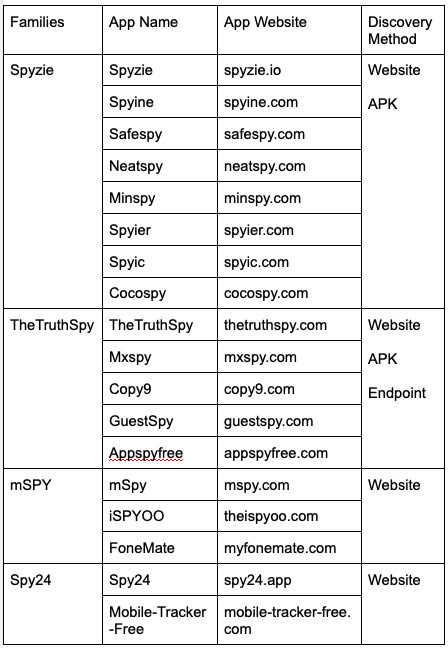
\includegraphics[width=\columnwidth]{figures/app_family.png}
%DIF <  \caption{App families identified while narrowing down the list of apps to study}
%DIF <  \label{tab:apps_family}
%DIF <  \end{figure}
\DIFaddbegin \bibitem{UseofSta91:online}
\BIBentryALTinterwordspacing
\DIFadd{Avast. (2022, 02) Use of stalkerware and spyware apps increase by 93\% since
  lockdown began in the uk. }[\DIFadd{Online}]\DIFadd{. Available:
  }\url{https://press.avast.com/use-of-stalkerware-and-spyware-apps-increase-by-93-since-lockdown-began-in-the-uk}
\BIBentrySTDinterwordspacing

\bibitem{chatterjee2018spyware}
\DIFadd{R.~Chatterjee, P.~Doerfler, H.~Orgad, S.~Havron, J.~Palmer, D.~Freed, K.~Levy,
  N.~Dell, D.~McCoy, and T.~Ristenpart, ``The spyware used in intimate partner
  violence,'' in }\emph{\DIFadd{Proceedings of the 2018 IEEE Symposium on Security and
  Privacy (SP)}}\DIFadd{.}\hskip \DIFadd{1em plus 0.5em minus 0.4em}\relax \DIFadd{IEEE, 2018, pp.
  441--458.
}

\bibitem{woodlock2017abuse}
\DIFadd{D.~Woodlock, ``The abuse of technology in domestic violence and stalking,''
  }\emph{\DIFadd{Violence against women}}\DIFadd{, vol.~23, no.~5, pp. 584--602, 2017.
}

\bibitem{HackerSt66:online}
\BIBentryALTinterwordspacing
\DIFadd{J.~Cox. (2022, 02) Hacker steals customers' text messages from android spyware
  company. }[\DIFadd{Online}]\DIFadd{. Available:
  }\url{https://www.vice.com/en/article/qvm44m/hacker-steals-text-messages-android-spyware-company-spyhuman}
\BIBentrySTDinterwordspacing

\bibitem{Companyt8:online}
\BIBentryALTinterwordspacing
\DIFadd{WAQAS. (2022, 02) Company that sells spyware to domestic abusers hacked.
  }[\DIFadd{Online}]\DIFadd{. Available:
  }\url{https://www.hackread.com/company-that-sells-spyware-to-domestic-abusers-hacked/}
\BIBentrySTDinterwordspacing

\bibitem{mSpybrea38:online}
\BIBentryALTinterwordspacing
\DIFadd{B.~Krebs. (2022, 02) mspy breach \- krebs on security. }[\DIFadd{Online}]\DIFadd{. Available:
  }\url{https://krebsonsecurity.com/tag/mspy-breach/}
\BIBentrySTDinterwordspacing

\bibitem{mSpyCybe86:online}
\BIBentryALTinterwordspacing
\DIFadd{C.~Insurance. (2022, 02) mspy - cyberinsurance.com. }[\DIFadd{Online}]\DIFadd{. Available:
  }\url{https://www.cyberinsurance.com/breaches/mspy/}
\BIBentrySTDinterwordspacing

\bibitem{Cerberus12:online}
\BIBentryALTinterwordspacing
\DIFadd{Rithvik. (2022, 02) Cerberus acknowledges data breach, states some usernames
  and encrypted passwords stolen. }[\DIFadd{Online}]\DIFadd{. Available:
  }\url{https://www.droid-life.com/2014/03/26/cerberus-data-breach/}
\BIBentrySTDinterwordspacing

\bibitem{Stalkerw59:online}
\BIBentryALTinterwordspacing
\DIFadd{L.~Franceschi-Bicchierai. (2022, 02) Stalkerware company flexispy calls
  catastrophic hack 'just some false news'. }[\DIFadd{Online}]\DIFadd{. Available:
  }\url{https://www.vice.com/en/article/xyjwpw/flexispy-calls-catastrophic-hack-just-some-false-news}
\BIBentrySTDinterwordspacing

\bibitem{HackerSt50:online}
\BIBentryALTinterwordspacing
\DIFadd{J.~Cox. (2022, 02) Hacker strikes 'stalkerware' companies, stealing alleged
  texts and gps locations of customers. }[\DIFadd{Online}]\DIFadd{. Available:
  }\url{https://www.vice.com/en/article/7x77ex/hacker-strikes-stalkerware-companies-stealing-alleged-texts-and-gps-locations-of-customers}
\BIBentrySTDinterwordspacing

\bibitem{Spywaref13:online}
\BIBentryALTinterwordspacing
\DIFadd{C.~Osborne. (2022, 02) Spyware firm spyfone leaves customer data, recordings
  exposed online. }[\DIFadd{Online}]\DIFadd{. Available:
  }\url{https://www.zdnet.com/article/spyware-firm-spyfone-leaves-customer-data-recordings-exposed-online/}
\BIBentrySTDinterwordspacing

\bibitem{RetinaXa98:online}
\BIBentryALTinterwordspacing
\DIFadd{Z.~Zorz. (2022, 02) Retina-x admits they have suffered a data breach - help net
  security. }[\DIFadd{Online}]\DIFadd{. Available:
  }\url{https://www.helpnetsecurity.com/2017/05/02/retina-x-data-breach/}
\BIBentrySTDinterwordspacing

\bibitem{Hackercl62:online}
\BIBentryALTinterwordspacing
\DIFadd{L.~Vaas. (2022, 02) Hacker claims spyware maker retina-x has been breached,
  again. }[\DIFadd{Online}]\DIFadd{. Available:
  }\url{https://nakedsecurity.sophos.com/2018/02/23/hacker-claims-spyware-maker-retina-x-has-been-breached-again/}
\BIBentrySTDinterwordspacing

\bibitem{IDOR62:online}
\BIBentryALTinterwordspacing
\DIFadd{Wikipedia. (2022, 08) Insecure direct object reference. }[\DIFadd{Online}]\DIFadd{. Available:
  }\url{https://en.wikipedia.org/wiki/Insecure_direct_object_reference}
\BIBentrySTDinterwordspacing

\bibitem{IDORCWE:online}
\BIBentryALTinterwordspacing
\DIFadd{C.~W. Enumeration. (2022, 08) Cwe - cwe-813: Owasp top ten 2010 category a4.
  }[\DIFadd{Online}]\DIFadd{. Available: }\url{https://cwe.mitre.org/data/definitions/813.html}
\BIBentrySTDinterwordspacing

\bibitem{howToJailbreakIphone:online}
\BIBentryALTinterwordspacing
\DIFadd{Z.~Whittaker. (2022, 02) How to jailbreak your iphone or ipod touch. }[\DIFadd{Online}]\DIFadd{.
  Available:
  }\url{https://www.digitaltrends.com/mobile/how-to-jailbreak-your-iphone/}
\BIBentrySTDinterwordspacing

\bibitem{esetandr4:online}
\BIBentryALTinterwordspacing
\DIFadd{L.~Stefanko. (2021, 05) Android stalkerware vulnerabilities. }[\DIFadd{Online}]\DIFadd{.
  Available:
  }\url{https://www.welivesecurity.com/wp-content/uploads/2021/05/eset_android_stalkerware.pdf}
\BIBentrySTDinterwordspacing

\bibitem{Tekstalk86:online}
\BIBentryALTinterwordspacing
\DIFadd{Te-k. (2022, 01) Te-k/stalkerware-indicators: Indicators of stalkerware apps.
  }[\DIFadd{Online}]\DIFadd{. Available: }\url{https://github.com/Te-k/stalkerware-indicators}
\BIBentrySTDinterwordspacing

\bibitem{pochat2018tranco}
\DIFadd{V.~L. Pochat, T.~Van~Goethem, S.~Tajalizadehkhoob, M.~Korczy}{\DIFadd{\'n}}\DIFadd{ski, and
  W.~Joosen, ``Tranco: A research-oriented top sites ranking hardened against
  manipulation,'' }\emph{\DIFadd{arXiv preprint arXiv:1806.01156}}\DIFadd{, 2018.
}

\bibitem{ApktoolA72:online}
\BIBentryALTinterwordspacing
\DIFadd{Apktool. (2022, 01) Apktool - a tool for reverse engineering 3rd party, closed,
  binary android apps. }[\DIFadd{Online}]\DIFadd{. Available:
  }\url{https://ibotpeaches.github.io/Apktool/}
\BIBentrySTDinterwordspacing

\bibitem{skylotja9:online}
\BIBentryALTinterwordspacing
\DIFadd{skylot. (2022, 01) skylot/jadx: Dex to java decompiler. }[\DIFadd{Online}]\DIFadd{. Available:
  }\url{https://github.com/skylot/jadx}
\BIBentrySTDinterwordspacing

\bibitem{Firebase21:online}
\BIBentryALTinterwordspacing
\DIFadd{Google. (2022, 02) Firebasemessagingservice. }[\DIFadd{Online}]\DIFadd{. Available:
  }\url{https://firebase.google.com/docs/reference/android/com/google/firebase/messaging/FirebaseMessagingService}
\BIBentrySTDinterwordspacing

\bibitem{yan2019understanding}
\DIFadd{Y.~Yan, Z.~Li, Q.~A. Chen, C.~Wilson, T.~Xu, E.~Zhai, Y.~Li, and Y.~Liu,
  ``Understanding and detecting overlay-based android malware at market
  scales,'' in }\emph{\DIFadd{Proceedings of the 17th Annual International Conference on
  Mobile Systems, Applications, and Services}}\DIFadd{, 2019, pp. 168--179.
}

\bibitem{Cameraca74:online}
\BIBentryALTinterwordspacing
\DIFadd{Google. (2021, 08) Camera capture sessions and requests. }[\DIFadd{Online}]\DIFadd{. Available:
  }\url{https://developer.android.com/training/camera2/capture-sessions-requests}
\BIBentrySTDinterwordspacing

\bibitem{SurfaceT78:online}
\BIBentryALTinterwordspacing
\DIFadd{------. (2022, 02) Surfacetexture. }[\DIFadd{Online}]\DIFadd{. Available:
  }\url{https://developer.android.com/reference/android/graphics/SurfaceTexture}
\BIBentrySTDinterwordspacing

\bibitem{WebViewA25:online}
\BIBentryALTinterwordspacing
\DIFadd{------. (2022, 02) Webview. }[\DIFadd{Online}]\DIFadd{. Available:
  }\url{https://developer.android.com/reference/android/webkit/WebView}
\BIBentrySTDinterwordspacing

\bibitem{MediaRec53:online}
\BIBentryALTinterwordspacing
\DIFadd{------. (2021, 08) Mediarecorder.audiosource. }[\DIFadd{Online}]\DIFadd{. Available:
  }\url{https://developer.android.com/reference/android/media/MediaRecorder.AudioSource}
\BIBentrySTDinterwordspacing

\bibitem{VOICECAL55:online}
\BIBentryALTinterwordspacing
\DIFadd{------. (2021, 08) Voice\_call audio source requires
  android.permission.capture\_audio\_output }[\DIFadd{37094464}] \DIFadd{- visible to public -
  issue tracker. }[\DIFadd{Online}]\DIFadd{. Available:
  }\url{https://issuetracker.google.com/issues/37094464}
\BIBentrySTDinterwordspacing

\bibitem{ViktorDe77:online}
\BIBentryALTinterwordspacing
\DIFadd{ViktorDegtyarev. (2021, 08) Viktordegtyarev/callreclib: Call recorder fix for
  android 7 and android 6. }[\DIFadd{Online}]\DIFadd{. Available:
  }\url{https://github.com/ViktorDegtyarev/CallRecLib}
\BIBentrySTDinterwordspacing

\bibitem{coplukAC3:online}
\BIBentryALTinterwordspacing
\DIFadd{Bitbucket. (2021, 08) copluk / acr / issues / \#2418 - }[\DIFadd{kb}] \DIFadd{android 9 (p) call
  recording issues. }[\DIFadd{Online}]\DIFadd{. Available:
  }\url{https://bitbucket.org/copluk/acr/issues/2418/kb-android-9-p-call-recording-issues}
\BIBentrySTDinterwordspacing

\bibitem{services10:online}
\BIBentryALTinterwordspacing
\DIFadd{Google. (2021, 08) services/audioflinger/audioflinger.cpp -
  platform/frameworks/av - git at google. }[\DIFadd{Online}]\DIFadd{. Available:
  }\url{https://android.googlesource.com/platform/frameworks/av/+/android-9.0.0_r30/services/audioflinger/AudioFlinger.cpp}
\BIBentrySTDinterwordspacing

\bibitem{Sharinga60:online}
\BIBentryALTinterwordspacing
\DIFadd{------. (2021, 08) Sharing audio input. }[\DIFadd{Online}]\DIFadd{. Available:
  }\url{https://developer.android.com/guide/topics/media/sharing-audio-input#accessibility_service_ordinary_app}
\BIBentrySTDinterwordspacing

\bibitem{fratantonio2017cloak}
\DIFadd{Y.~Fratantonio, C.~Qian, S.~P. Chung, and W.~Lee, ``Cloak and dagger: from two
  permissions to complete control of the ui feedback loop,'' in
  }\emph{\DIFadd{Proceedings of the 2017 IEEE Symposium on Security and Privacy
  (SP)}}\DIFadd{.}\hskip \DIFadd{1em plus 0.5em minus 0.4em}\relax \DIFadd{IEEE, 2017, pp. 1041--1057.
}

\bibitem{kraunelis2013malware}
\DIFadd{J.~Kraunelis, Y.~Chen, Z.~Ling, X.~Fu, and W.~Zhao, ``On malware leveraging the
  android accessibility framework,'' in }\emph{\DIFadd{Proceedings of the International
  Conference on Mobile and Ubiquitous Systems: Computing, Networking, and
  Services}}\DIFadd{.}\hskip \DIFadd{1em plus 0.5em minus 0.4em}\relax \DIFadd{Springer, 2013, pp.
  512--523.
}

\bibitem{jang2014a11y}
\DIFadd{Y.~Jang, C.~Song, S.~P. Chung, T.~Wang, and W.~Lee, ``A11y attacks: Exploiting
  accessibility in operating systems,'' in }\emph{\DIFadd{Proceedings of the 2014 ACM
  SIGSAC Conference on Computer and Communications Security}}\DIFadd{, 2014, pp.
  103--115.
}

\bibitem{diao2019kindness}
\DIFadd{W.~Diao, Y.~Zhang, L.~Zhang, Z.~Li, F.~Xu, X.~Pan, X.~Liu, J.~Weng, K.~Zhang,
  and X.~Wang, ``Kindness is a risky business: on the usage of the
  accessibility apis in android,'' in }\emph{\DIFadd{Proceedings of the 22nd
  International Symposium on Research in Attacks, Intrusions and Defenses
  ($\{$RAID$\}$ 2019)}}\DIFadd{, 2019, pp. 261--275.
}

\bibitem{kalysch2018android}
\DIFadd{A.~Kalysch, D.~Bove, and T.~M}{\DIFadd{\"u}}\DIFadd{ller, ``How android's ui security is
  undermined by accessibility,'' in }\emph{\DIFadd{Proceedings of the 2nd Reversing and
  Offensive-oriented Trends Symposium}}\DIFadd{, 2018, pp. 1--10.
}

\bibitem{huang2021a11y}
\DIFadd{J.~Huang, M.~Backes, and S.~Bugiel, ``A11y and privacy don't have to be
  mutually exclusive: Constraining accessibility service misuse on android,''
  in }\emph{\DIFadd{Proceedings of the 30th USENIX Security Symposium}}\DIFadd{, 2021.
}

\bibitem{naseri2019accessileaks}
\DIFadd{M.~Naseri, N.~P. Borges~Jr, A.~Zeller, and R.~Rouvoy, ``Accessileaks:
  investigating privacy leaks exposed by the android accessibility service,''
  2019.
}

\bibitem{VB2019Za6:online}
\BIBentryALTinterwordspacing
\DIFadd{R.~Gibson. (2019, 10) Countering tech abuse together. }[\DIFadd{Online}]\DIFadd{. Available:
  }\url{https://www.virusbulletin.com/uploads/pdf/conference_slides/2019/VB2019-ZakorzhevskyG.pdf}
\BIBentrySTDinterwordspacing

\bibitem{ReadUnre55:online}
\BIBentryALTinterwordspacing
\DIFadd{R.~Unread. (2022, 08) Read unread: unseen hide and read, last seenonline.
  }[\DIFadd{Online}]\DIFadd{. Available:
  }\url{https://play.google.com/store/apps/details?id=com.read.unread.last.seen.unseen.hidden.chat}
\BIBentrySTDinterwordspacing

\bibitem{androidH20:online}
\BIBentryALTinterwordspacing
\DIFadd{Stackoverflow. (2021, 10) android - how to use mediaprojection to capture
  screen in a service? - stack overflow. }[\DIFadd{Online}]\DIFadd{. Available:
  }\url{https://stackoverflow.com/questions/51182557/how-to-use-mediaprojection-to-capture-screen-in-a-service}
\BIBentrySTDinterwordspacing

\bibitem{Restrict50:online}
\BIBentryALTinterwordspacing
\DIFadd{Google. (2021, 12) Restrictions on starting activities from the background.
  }[\DIFadd{Online}]\DIFadd{. Available:
  }\url{https://developer.android.com/guide/components/activities/background-starts}
\BIBentrySTDinterwordspacing

\bibitem{Accessib97:online}
\BIBentryALTinterwordspacing
\DIFadd{------. (2021, 12) Accessibilityservice. }[\DIFadd{Online}]\DIFadd{. Available:
  }\url{\DIFadd{https://developer.android.com/reference/android/accessibilityservice/AccessibilityService#takeScreenshot(int,%DIF > 20java.util.concurrent.Executor,%20android.accessibilityservice.AccessibilityService.TakeScreenshotCallback)}
}\BIBentrySTDinterwordspacing

\bibitem{Privacyc52:online}
\BIBentryALTinterwordspacing
\DIFadd{------. (2021, 11) Privacy changes in android 10. }[\DIFadd{Online}]\DIFadd{. Available:
  }\url{https://developer.android.com/about/versions/10/privacy/changes}
\BIBentrySTDinterwordspacing

\bibitem{SolvedCl34:online}
\BIBentryALTinterwordspacing
\DIFadd{Joaoapps. (2022, 08) Solved - clipboard monitor/listener no longer works on
  android 10. }[\DIFadd{Online}]\DIFadd{. Available:
  }\url{https://forum.joaoapps.com/index.php?threads/clipboard-monitor-listener-no-longer-works-on-android-10.49808/}
\BIBentrySTDinterwordspacing

\bibitem{HowcanIt38:online}
\BIBentryALTinterwordspacing
\DIFadd{Google. (2021, 08) How can i turn off camera shutter sound - google pixel
  community. }[\DIFadd{Online}]\DIFadd{. Available:
  }\url{https://support.google.com/pixelphone/thread/69083830/how-can-i-turn-off-camera-shutter-sound?hl=en}
\BIBentrySTDinterwordspacing

\bibitem{petracca2015audroid}
\DIFadd{G.~Petracca, Y.~Sun, T.~Jaeger, and A.~Atamli, ``Audroid: Preventing attacks on
  audio channels in mobile devices,'' in }\emph{\DIFadd{Proceedings of the 31st Annual
  Computer Security Applications Conference}}\DIFadd{, 2015, pp. 181--190.
}

\bibitem{whataret1:online}
\BIBentryALTinterwordspacing
\DIFadd{Stackoverflow. (2021, 11) what are the uses of main, default and launcher in
  manifest file in android - stack overflow. }[\DIFadd{Online}]\DIFadd{. Available:
  }\url{https://stackoverflow.com/questions/9721030/what-are-the-uses-of-main-default-and-launcher-in-manifest-file-in-android}
\BIBentrySTDinterwordspacing

\bibitem{shan2018self}
\DIFadd{Z.~Shan, I.~Neamtiu, and R.~Samuel, ``Self-hiding behavior in android apps:
  detection and characterization,'' in }\emph{\DIFadd{Proceedings of the 40th
  International Conference on Software Engineering}}\DIFadd{, 2018, pp. 728--739.
}

\bibitem{IntentAn33:online}
\BIBentryALTinterwordspacing
\DIFadd{Google. (2022, 02) Intent. }[\DIFadd{Online}]\DIFadd{. Available:
  }\url{https://developer.android.com/reference/android/content/Intent#CATEGORY_LAUNCHER}
\BIBentrySTDinterwordspacing

\bibitem{Launcher79:online}
\BIBentryALTinterwordspacing
\DIFadd{------. (2021, 08) Launcherapps. }[\DIFadd{Online}]\DIFadd{. Available:
  }\url{\DIFadd{https://developer.android.com/reference/android/content/pm/LauncherApps#getActivityList(java.lang.String,%DIF > 20android.os.UserHandle)}
}\BIBentrySTDinterwordspacing

\bibitem{Launcher48:online}
\BIBentryALTinterwordspacing
\DIFadd{LauncherAppsService. (2022, 08) Launcherappsservice.java - android code search.
  }[\DIFadd{Online}]\DIFadd{. Available:
  }\url{https://cs.android.com/android/platform/superproject/+/android-10.0.0_r1:frameworks/base/services/core/java/com/android/server/pm/LauncherAppsService.java;l=439}
\BIBentrySTDinterwordspacing

\bibitem{CreateDe16:online}
\BIBentryALTinterwordspacing
\DIFadd{Google. (2022, 02) Create deep links to app content. }[\DIFadd{Online}]\DIFadd{. Available:
  }\url{https://developer.android.com/training/app-links/deep-linking}
\BIBentrySTDinterwordspacing

\bibitem{Appwidge49:online}
\BIBentryALTinterwordspacing
\DIFadd{------. (2022, 02) App widgets overview. }[\DIFadd{Online}]\DIFadd{. Available:
  }\url{https://developer.android.com/guide/topics/appwidgets/overview}
\BIBentrySTDinterwordspacing

\bibitem{Recentss9:online}
\BIBentryALTinterwordspacing
\DIFadd{------. (2021, 11) Recents screen. }[\DIFadd{Online}]\DIFadd{. Available:
  }\url{https://developer.android.com/guide/components/activities/recents}
\BIBentrySTDinterwordspacing

\bibitem{zhou2020demystifying}
\DIFadd{H.~Zhou, H.~Wang, Y.~Zhou, X.~Luo, Y.~Tang, L.~Xue, and T.~Wang, ``Demystifying
  diehard android apps,'' in }\emph{\DIFadd{Proceedings of the 35th IEEE/ACM
  International Conference on Automated Software Engineering (ASE)}}\DIFadd{.}\hskip \DIFadd{1em
  plus 0.5em minus 0.4em}\relax \DIFadd{IEEE, 2020, pp. 187--198.
}

\bibitem{activity72:online}
\BIBentryALTinterwordspacing
\DIFadd{Google. (2021, 11) <activity>. }[\DIFadd{Online}]\DIFadd{. Available:
  }\url{https://developer.android.com/guide/topics/manifest/activity-element#exclude}
\BIBentrySTDinterwordspacing

\bibitem{IntentAn90:online}
\BIBentryALTinterwordspacing
\DIFadd{------. (2022, 02) Intent. }[\DIFadd{Online}]\DIFadd{. Available:
  }\url{https://developer.android.com/reference/android/content/Intent#FLAG_ACTIVITY_EXCLUDE_FROM_RECENTS}
\BIBentrySTDinterwordspacing

\bibitem{shan2019device}
\DIFadd{Z.~Shan, R.~Samuel, and I.~Neamtiu, ``Device administrator use and abuse in
  android: Detection and characterization,'' in }\emph{\DIFadd{Proceedings of the 25th
  Annual International Conference on Mobile Computing and Networking}}\DIFadd{, 2019,
  pp. 1--16.
}

\bibitem{aljarrah2016maintaining}
\DIFadd{A.~AlJarrah and M.~Shehab, ``Maintaining user interface integrity on android,''
  in }\emph{\DIFadd{Proceedings of the 40th Annual Computer Software and Applications
  Conference (COMPSAC)}}\DIFadd{, vol.~1.}\hskip \DIFadd{1em plus 0.5em minus 0.4em}\relax \DIFadd{IEEE,
  2016, pp. 449--458.
}

\bibitem{shao2019lightweight}
\DIFadd{Y.~Shao, R.~Wang, X.~Chen, A.~M. Azab, and Z.~M. Mao, ``A lightweight framework
  for fine-grained lifecycle control of android applications,'' in
  }\emph{\DIFadd{Proceedings of the Fourteenth EuroSys Conference 2019}}\DIFadd{, 2019, pp.
  1--14.
}

\bibitem{JobSched94:online}
\BIBentryALTinterwordspacing
\DIFadd{Google. (2021, 08) Jobscheduler. }[\DIFadd{Online}]\DIFadd{. Available:
  }\url{https://developer.android.com/reference/android/app/job/JobScheduler}
\BIBentrySTDinterwordspacing

\bibitem{AlarmMan39:online}
\BIBentryALTinterwordspacing
\DIFadd{------. (2021, 08) Alarmmanager. }[\DIFadd{Online}]\DIFadd{. Available:
  }\url{https://developer.android.com/reference/android/app/AlarmManager}
\BIBentrySTDinterwordspacing

\bibitem{Broadcas25:online}
\BIBentryALTinterwordspacing
\DIFadd{------. (2022, 06) Broadcasts overview. }[\DIFadd{Online}]\DIFadd{. Available:
  }\url{https://developer.android.com/guide/components/broadcasts}
\BIBentrySTDinterwordspacing

\bibitem{Implicit72:online}
\BIBentryALTinterwordspacing
\DIFadd{------. (2022, 06) Implicit broadcast exceptions. }[\DIFadd{Online}]\DIFadd{. Available:
  }\url{https://developer.android.com/guide/components/broadcast-exceptions}
\BIBentrySTDinterwordspacing

\bibitem{AndroidA0:online}
\BIBentryALTinterwordspacing
\DIFadd{Accountable2you. (2022, 08) Android accessibility keeps turning off
  accountable2you - accountable2you support. }[\DIFadd{Online}]\DIFadd{. Available:
  }\url{\DIFadd{https://support.accountable2you.com/article/754-android-accessibility-keeps-turning-off-accountable2you#:~:text=If%DIF > 20you%20notice%20that%20Accountable2You,to%20customize%20these%20battery%20settings.}
}\BIBentrySTDinterwordspacing

\bibitem{Accessib46:online}
\BIBentryALTinterwordspacing
\DIFadd{Stackexchange. (2022, 08) Accessibility services gets disabled automatically -
  android enthusiasts stack exchange. }[\DIFadd{Online}]\DIFadd{. Available:
  }\url{https://android.stackexchange.com/questions/137195/accessibility-services-gets-disabled-automatically}
\BIBentrySTDinterwordspacing

\bibitem{fernandes2016android}
\DIFadd{E.~Fernandes, Q.~A. Chen, J.~Paupore, G.~Essl, J.~A. Halderman, Z.~M. Mao, and
  A.~Prakash, ``Android ui deception revisited: Attacks and defenses,'' in
  }\emph{\DIFadd{International Conference on Financial Cryptography and Data
  Security}}\DIFadd{.}\hskip \DIFadd{1em plus 0.5em minus 0.4em}\relax \DIFadd{Springer, 2016, pp. 41--59.
}

\bibitem{HowtoDis42:online}
\BIBentryALTinterwordspacing
\DIFadd{P.~Mitchell. (2021, 04) How to disable auto-start apps on android - techcult.
  }[\DIFadd{Online}]\DIFadd{. Available:
  }\url{https://techcult.com/how-to-disable-auto-start-apps-on-android/}
\BIBentrySTDinterwordspacing

\bibitem{Stalking85:online}
\BIBentryALTinterwordspacing
\DIFadd{A.~Langton. (2019, 12) Stalking stalkerware: A deep dive into flexispy.
  }[\DIFadd{Online}]\DIFadd{. Available:
  }\url{https://blogs.juniper.net/en-us/threat-research/stalking-stalkerware-a-deep-dive-into-flexispy-2}
\BIBentrySTDinterwordspacing

\bibitem{santhanam2022scraping}
\DIFadd{P.~Santhanam, H.~Dang, Z.~Shan, and I.~Neamtiu, ``Scraping sticky leftovers:
  App user information left on servers after account deletion,'' in
  }\emph{\DIFadd{Proceedings of the 2022 IEEE Symposium on Security and Privacy
  (SP)}}\DIFadd{.}\hskip \DIFadd{1em plus 0.5em minus 0.4em}\relax \DIFadd{IEEE, 2022, pp. 2145--2160.
}

\bibitem{SpappSMSCommands:online}
\BIBentryALTinterwordspacing
\DIFadd{S.~Monitoring. (2022, 02) Available sms commands for spapp. }[\DIFadd{Online}]\DIFadd{.
  Available: }\url{https://www.spappmonitoring.com/news/display/live_control}
\BIBentrySTDinterwordspacing

\bibitem{FlexispySMSCommands:online}
\BIBentryALTinterwordspacing
\DIFadd{Flexispy. (2022, 02) Remote commands for flexispy. }[\DIFadd{Online}]\DIFadd{. Available:
  }\url{https://portal.flexispy.com/help/en/misc/sms-commands.html}
\BIBentrySTDinterwordspacing

\bibitem{PowerPoi79:online}
\BIBentryALTinterwordspacing
\DIFadd{J.~Dalman. (2015, 07) Commercial spyware --- detecting the undetectable.
  }[\DIFadd{Online}]\DIFadd{. Available:
  }\url{https://www.blackhat.com/docs/us-15/materials/us-15-Dalman-Commercial-Spyware-Detecting-The-Undetectable.pdf}
\BIBentrySTDinterwordspacing

\bibitem{SpyvsSpy59:online}
\BIBentryALTinterwordspacing
\DIFadd{m.~robinson and c.~taylor. (2020, 02) Spy vs spy: Spying on mobile device
  spyware. }[\DIFadd{Online}]\DIFadd{. Available:
  }\url{\DIFadd{https://media.defcon.org/DEF%DIF > 20CON%2020/DEF%20CON%2020%20presentations/DEF%20CON%2020%20-%20Robinson-Spy-vs-Spy.pdf}
}\BIBentrySTDinterwordspacing

\bibitem{ANewWave1:online}
\BIBentryALTinterwordspacing
\DIFadd{Zscaler. (2019, 11) A new wave of stalkerware apps. }[\DIFadd{Online}]\DIFadd{. Available:
  }\url{https://www.zscaler.com/blogs/security-research/new-wave-stalkerware-apps}
\BIBentrySTDinterwordspacing

\bibitem{Whyyoush17:online}
\BIBentryALTinterwordspacing
\DIFadd{------. (2018, 10) Why you shouldn't trust "safe" spying apps. }[\DIFadd{Online}]\DIFadd{.
  Available:
  }\url{https://www.zscaler.com/blogs/security-research/why-you-shouldnt-trust-safe-spying-apps}
\BIBentrySTDinterwordspacing

\bibitem{ReverseE12:online}
\BIBentryALTinterwordspacing
\DIFadd{M.~Grassi. (2014, 10) Reverse engineering of a commercial spyware for ios and
  android - speaker deck. }[\DIFadd{Online}]\DIFadd{. Available:
  }\url{https://speakerdeck.com/marcograss/reverse-engineering-of-a-commercial-spyware-for-ios-and-android}
\BIBentrySTDinterwordspacing

\bibitem{YourInfo19:online}
\BIBentryALTinterwordspacing
\DIFadd{C.~Admin. (2021, 11) Your infosec s.w.a.t team. }[\DIFadd{Online}]\DIFadd{. Available:
  }\url{https://cyberarch.eu/our-blog/pegasus-spyware-analysis/}
\BIBentrySTDinterwordspacing

\bibitem{FlexSpyA1:online}
\BIBentryALTinterwordspacing
\DIFadd{C.~M. of~Death. (2017, 04) Flexspy application analysis. }[\DIFadd{Online}]\DIFadd{. Available:
  }\url{http://www.cybermerchantsofdeath.com/blog/2017/04/22/FlexiSpy.html}
\BIBentrySTDinterwordspacing

\bibitem{diskurse89:online}
\BIBentryALTinterwordspacing
\DIFadd{diskurse. (2022, 01) diskurse/android-stalkerware: Various analysis of android
  stalkerware. }[\DIFadd{Online}]\DIFadd{. Available:
  }\url{https://github.com/diskurse/android-stalkerware}
\BIBentrySTDinterwordspacing

\bibitem{SpywareP46:online}
\BIBentryALTinterwordspacing
\DIFadd{Zscaler. (05, 2022) Spyware presence in enterprise networks blog. }[\DIFadd{Online}]\DIFadd{.
  Available:
  }\url{https://www.zscaler.com/blogs/security-research/spyware-presence-enterprise-networks}
\BIBentrySTDinterwordspacing

\bibitem{Androida91:online}
\BIBentryALTinterwordspacing
\DIFadd{S.~Sidor. (2022, 05) Android: apps can take photos with your phone without you
  knowing. - mobile security - romanian security team. }[\DIFadd{Online}]\DIFadd{. Available:
  }\url{https://rstforums.com/forum/topic/79016-android-apps-can-take-photos-with-your-phone-without-you-knowing/}
\BIBentrySTDinterwordspacing

\bibitem{parsons2019predator}
\DIFadd{C.~Parsons, A.~Molnar, J.~Dalek, J.~Knockel, M.~Kenyon, B.~Haselton, C.~Khoo,
  and R.~Deibert, ``The predator in your pocket: A multidisciplinary assessment
  of the stalkerware application industry,'' 2019.
}

\bibitem{harkin2019consumer}
\DIFadd{D.~Harkin and A.~Molnar, ``The consumer spyware industry: an australian-based
  analysis of the threats of consumer spyware,'' 2019.
}

\bibitem{harkin2020commodification}
\DIFadd{D.~Harkin, A.~Molnar, and E.~Vowles, ``The commodification of mobile phone
  surveillance: An analysis of the consumer spyware industry,'' }\emph{\DIFadd{Crime,
  media, culture}}\DIFadd{, vol.~16, no.~1, pp. 33--60, 2020.
}

\bibitem{pierazzi2020data}
\DIFadd{F.~Pierazzi, G.~Mezzour, Q.~Han, M.~Colajanni, and V.~Subrahmanian, ``A
  data-driven characterization of modern android spyware,'' }\emph{\DIFadd{ACM
  Transactions on Management Information Systems (TMIS)}}\DIFadd{, vol.~11, no.~1, pp.
  1--38, 2020.
}

\bibitem{feal2020angel}
{\DIFadd{\'A}}\DIFadd{.~Feal, P.~Calciati, N.~Vallina-Rodriguez, C.~Troncoso, and A.~Gorla,
  ``Angel or devil? a privacy study of mobile parental control apps,''
  }\emph{\DIFadd{Proceedings of Privacy Enhancing Technologies}}\DIFadd{, vol. 2020, no.~2, pp.
  314--335, 2020.
}

\bibitem{harkin2021operating}
\DIFadd{D.~Harkin and A.~Molnar, ``Operating-system design and its implications for
  victims of family violence: the comparative threat of smart phone spyware for
  android versus iphone users,'' }\emph{\DIFadd{Violence against women}}\DIFadd{, vol.~27, no.
  6-7, pp. 851--875, 2021.
}

\bibitem{ch33r10S37:online}
\BIBentryALTinterwordspacing
\DIFadd{ch33r10. (2022, 02) ch33r10/stalkerware. }[\DIFadd{Online}]\DIFadd{. Available:
  }\url{https://github.com/ch33r10/Stalkerware}
\BIBentrySTDinterwordspacing

\bibitem{almansoori2022global}
\DIFadd{M.~Almansoori, A.~Gallardo, J.~Poveda, A.~Ahmed, and R.~Chatterjee, ``A global
  survey of android dual-use applications used in intimate partner
  surveillance,'' }\emph{\DIFadd{Proceedings of Privacy Enhancing Technologies}}\DIFadd{, vol.~4,
  pp. 120--139, 2022.
}

\bibitem{han2021towards}
\DIFadd{Y.~Han, K.~A. Roundy, and A.~Tamersoy, ``Towards stalkerware detection with
  precise warnings,'' in }\emph{\DIFadd{Annual Computer Security Applications
  Conference}}\DIFadd{, 2021, pp. 957--969.
}

\bibitem{saroiu2004measurement}
\DIFadd{S.~Saroiu, S.~D. Gribble, and H.~M. Levy, ``Measurement and analysis of spyware
  in a university environment.'' in }\emph{\DIFadd{NSDI}}\DIFadd{, 2004, pp. 141--153.
}

\bibitem{egele2007dynamic}
\DIFadd{M.~Egele, C.~Kruegel, E.~Kirda, H.~Yin, and D.~Song, ``Dynamic spyware
  analysis,'' 2007.
}

\bibitem{roundy2020many}
\DIFadd{K.~A. Roundy, P.~B. Mendelberg, N.~Dell, D.~McCoy, D.~Nissani, T.~Ristenpart,
  and A.~Tamersoy, ``The many kinds of creepware used for interpersonal
  attacks,'' in }\emph{\DIFadd{Proceedings of the 2020 IEEE Symposium on Security and
  Privacy (SP '20)}}\DIFadd{.}\hskip \DIFadd{1em plus 0.5em minus 0.4em}\relax \DIFadd{IEEE, 2020, pp.
  626--643.
}

\bibitem{wang2006netspy}
\DIFadd{H.~Wang, S.~Jha, and V.~Ganapathy, ``Netspy: Automatic generation of spyware
  signatures for nids,'' in }\emph{\DIFadd{Proceedings of the 22nd Annual Computer
  Security Applications Conference (ACSAC'06)}}\DIFadd{.}\hskip \DIFadd{1em plus 0.5em minus
  0.4em}\relax \DIFadd{IEEE, 2006, pp. 99--108.
}

\bibitem{moshchuk2006crawler}
\DIFadd{A.~Moshchuk, T.~Bragin, S.~D. Gribble, and H.~M. Levy, ``A crawler-based study
  of spyware in the web.'' in }\emph{\DIFadd{NDSS}}\DIFadd{, vol.~1, 2006, p.~2.
}

\bibitem{randall2020trufflehunter}
\DIFadd{A.~Randall, E.~Liu, G.~Akiwate, R.~Padmanabhan, G.~M. Voelker, S.~Savage, and
  A.~Schulman, ``Trufflehunter: Cache snooping rare domains at large public dns
  resolvers,'' in }\emph{\DIFadd{Proceedings of the ACM Internet Measurement
  Conference}}\DIFadd{, 2020, pp. 50--64.
}

\bibitem{havron2019clinical}
\DIFadd{S.~Havron, D.~Freed, R.~Chatterjee, D.~McCoy, N.~Dell, and T.~Ristenpart,
  ``Clinical computer security for victims of intimate partner violence,'' in
  }\emph{\DIFadd{Proceedings of the 28th USENIX Security Symposium}}\DIFadd{, 2019, pp. 105--122.
}

\bibitem{freed2019my}
\DIFadd{D.~Freed, S.~Havron, E.~Tseng, A.~Gallardo, R.~Chatterjee, T.~Ristenpart, and
  N.~Dell, ``" is my phone hacked?" analyzing clinical computer security
  interventions with survivors of intimate partner violence,''
  }\emph{\DIFadd{Proceedings of the ACM on Human-Computer Interaction}}\DIFadd{, vol.~3, no.
  CSCW, pp. 1--24, 2019.
}

\bibitem{tseng2020tools}
\DIFadd{E.~Tseng, R.~Bellini, N.~McDonald, M.~Danos, R.~Greenstadt, D.~McCoy, N.~Dell,
  and T.~Ristenpart, ``The tools and tactics used in intimate partner
  surveillance: An analysis of online infidelity forums,'' in }\emph{\DIFadd{Proceedings
  of the 29th USENIX Security Symposium}}\DIFadd{, 2020, pp. 1893--1909.
}

\bibitem{thomas2021sok}
\DIFadd{K.~Thomas, D.~Akhawe, M.~Bailey, D.~Boneh, E.~Bursztein, S.~Consolvo, N.~Dell,
  Z.~Durumeric, P.~G. Kelley, D.~Kumar }\emph{\DIFadd{et~al.}}\DIFadd{, ``Sok: Hate, harassment,
  and the changing landscape of online abuse,'' in }\emph{\DIFadd{Proceedings of the
  2021 IEEE Symposium on Security and Privacy (SP)}}\DIFadd{.}\hskip \DIFadd{1em plus 0.5em minus
  0.4em}\relax \DIFadd{IEEE, 2021, pp. 247--267.
}

\bibitem{freed2018stalker}
\DIFadd{D.~Freed, J.~Palmer, D.~Minchala, K.~Levy, T.~Ristenpart, and N.~Dell, ``“a
  stalker's paradise” how intimate partner abusers exploit technology,'' in
  }\emph{\DIFadd{Proceedings of the 2018 CHI conference on human factors in computing
  systems}}\DIFadd{, 2018, pp. 1--13.
}

\bibitem{fraser2010new}
\DIFadd{C.~Fraser, E.~Olsen, K.~Lee, C.~Southworth, and S.~Tucker, ``The new age of
  stalking: Technological implications for stalking,'' }\emph{\DIFadd{Juvenile and
  family court journal}}\DIFadd{, vol.~61, no.~4, pp. 39--55, 2010.
}

\bibitem{shimizu2013domestic}
\DIFadd{A.~Shimizu, ``Domestic violence in the digital age: Towards the creation of a
  comprehensive cyberstalking statute,'' }\emph{\DIFadd{Berkeley J. Gender L. \& Just.}}\DIFadd{,
  vol.~28, p. 116, 2013.
}

\bibitem{southworth2005high}
\DIFadd{C.~Southworth, S.~Dawson, C.~Fraser, and S.~Tucker, ``A high-tech twist on
  abuse: Technology, intimate partner stalking, and advocacy,'' }\emph{\DIFadd{Violence
  Against Women Online Resources}}\DIFadd{, 2005.
}

\bibitem{southworth2006technology}
\DIFadd{C.~Southworth and S.~Tucker, ``Technology, stalking and domestic violence
  victims,'' }\emph{\DIFadd{Miss. LJ}}\DIFadd{, vol.~76, p. 667, 2006.
}

\bibitem{dragiewicz2019domestic}
\DIFadd{M.~Dragiewicz, B.~Harris, D.~Woodlock, M.~Salter, H.~Easton, A.~Lynch,
  H.~Campbell, J.~Leach, and L.~Milne, ``Domestic violence and communication
  technology: Survivor experiences of intrusion, surveillance, and identity
  crime,'' 2019.
}

\bibitem{mayrhofer2021android}
\DIFadd{R.~Mayrhofer, J.~V. Stoep, C.~Brubaker, and N.~Kralevich, ``The android
  platform security model,'' }\emph{\DIFadd{ACM Transactions on Privacy and Security
  (TOPS)}}\DIFadd{, vol.~24, no.~3, pp. 1--35, 2021.
}

\bibitem{motherboardstalkerwaremarket}
\BIBentryALTinterwordspacing
\DIFadd{V.~Motherboard. (2017) Inside the 'stalkerware' surveillance market, where
  ordinary people tap each other's phones. }[\DIFadd{Online}]\DIFadd{. Available:
  }\url{https://www.vice.com/en_us/article/53vm7n/inside-stalkerware-surveillance-market-flexispy-retina-x}
\BIBentrySTDinterwordspacing

\bibitem{pan2018panoptispy}
\DIFadd{E.~Pan, J.~Ren, M.~Lindorfer, C.~Wilson, and D.~Choffnes, ``Panoptispy:
  Characterizing audio and video exfiltration from android applications,''
  }\emph{\DIFadd{Proceedings of Privacy Enhancing Technologies}}\DIFadd{, vol. 2018, no.~4, pp.
  33--50, 2018.
}

\bibitem{luo2011attacks}
\DIFadd{T.~Luo, H.~Hao, W.~Du, Y.~Wang, and H.~Yin, ``Attacks on webview in the android
  system,'' in }\emph{\DIFadd{Proceedings of the 27th Annual Computer Security
  Applications Conference}}\DIFadd{, 2011, pp. 343--352.
}

\bibitem{chin2013bifocals}
\DIFadd{E.~Chin and D.~Wagner, ``Bifocals: Analyzing webview vulnerabilities in android
  applications,'' in }\emph{\DIFadd{Proceedings of the International Workshop on
  Information Security Applications}}\DIFadd{.}\hskip \DIFadd{1em plus 0.5em minus 0.4em}\relax
  \DIFadd{Springer, 2013, pp. 138--159.
}

\bibitem{neugschwandtner2013view}
\DIFadd{M.~Neugschwandtner, M.~Lindorfer, and C.~Platzer, ``A view to a
  kill:$\{$WebView$\}$ exploitation,'' in }\emph{\DIFadd{Proceedings of the 6th USENIX
  Workshop on Large-Scale Exploits and Emergent Threats (LEET 13)}}\DIFadd{, 2013.
}

\bibitem{ZhangIdentity2022}
\BIBentryALTinterwordspacing
\DIFadd{L.~Zhang, Z.~Zhang, A.~Liu, Y.~Cao, X.~Zhang, Y.~Chen, Y.~Zhang, G.~Yang, and
  M.~Yang, ``Identity confusion in }{\DIFadd{WebView-based}} \DIFadd{mobile app-in-app
  ecosystems,'' in }\emph{\DIFadd{Proceedings of the 31st USENIX Security
  Symposium}}\DIFadd{.}\hskip \DIFadd{1em plus 0.5em minus 0.4em}\relax \DIFadd{Boston, MA: USENIX
  Association, Aug. 2022, pp. 1597--1613. }[\DIFadd{Online}]\DIFadd{. Available:
  }\url{https://www.usenix.org/conference/usenixsecurity22/presentation/zhang-lei}
\BIBentrySTDinterwordspacing

\bibitem{pham2019hidemyapp}
\DIFadd{A.~Pham, I.~Dacosta, E.~Losiouk, J.~Stephan, K.~Huguenin, and J.-P. Hubaux,
  ``$\{$HideMyApp$\}$: Hiding the presence of sensitive apps on android,'' in
  }\emph{\DIFadd{Proceedings of 28th USENIX Security Symposium (USENIX Security 19)}}\DIFadd{, 08
  2019, pp. 711--728.
}

\bibitem{dojstealthgenie}
\BIBentryALTinterwordspacing
\DIFadd{D.~of~Justice. (2022, 02) Pakistani man indicted for selling 'stealthgenie'
  spyware app. }[\DIFadd{Online}]\DIFadd{. Available:
  }\url{https://www.justice.gov/opa/pr/pakistani-man-indicted-selling-stealthgenie-spyware-app}
\BIBentrySTDinterwordspacing

\bibitem{mccoy2012priceless}
\DIFadd{D.~McCoy, H.~Dharmdasani, C.~Kreibich, G.~M. Voelker, and S.~Savage,
  ``Priceless: The role of payments in abuse-advertised goods,'' in
  }\emph{\DIFadd{Proceedings of the 2012 ACM conference on Computer and communications
  security}}\DIFadd{, 2012, pp. 845--856.
}

\bibitem{FTCFinal26:online}
\BIBentryALTinterwordspacing
\DIFadd{FTC. (2022, 02) Ftc finalizes order banning stalkerware provider from spyware
  business. }[\DIFadd{Online}]\DIFadd{. Available:
  }\url{https://www.ftc.gov/news-events/press-releases/2021/12/ftc-finalizes-order-banning-stalkerware-provider-spyware-business}
\BIBentrySTDinterwordspacing

\bibitem{SuarezTangil2013Dendroid}
\BIBentryALTinterwordspacing
\DIFadd{G.~Suarez-Tangil, J.~E. Tapiador, P.~Peris-Lopez, and J.~Blasco, ``Dendroid: A
  text mining approach to analyzing and classifying code structures in android
  malware families,'' }\emph{\DIFadd{Expert Syst. Appl.}}\DIFadd{, vol.~41, no.~4, p.
  1104–1117, mar 2014. }[\DIFadd{Online}]\DIFadd{. Available:
  }\url{https://doi.org/10.1016/j.eswa.2013.07.106}
\BIBentrySTDinterwordspacing

\bibitem{Zhang2014Semantics}
\BIBentryALTinterwordspacing
\DIFadd{M.~Zhang, Y.~Duan, H.~Yin, and Z.~Zhao, ``Semantics-aware android malware
  classification using weighted contextual api dependency graphs,'' in
  }\emph{\DIFadd{Proceedings of the 2014 ACM SIGSAC Conference on Computer and
  Communications Security}}\DIFadd{, ser. CCS '14.}\hskip \DIFadd{1em plus 0.5em minus
  0.4em}\relax \DIFadd{New York, NY, USA: Association for Computing Machinery, 2014, p.
  1105–1116. }[\DIFadd{Online}]\DIFadd{. Available:
  }\url{https://doi.org/10.1145/2660267.2660359}
\BIBentrySTDinterwordspacing

\bibitem{deshotels2014droidlegacy}
\DIFadd{L.~Deshotels, V.~Notani, and A.~Lakhotia, ``Droidlegacy: Automated familial
  classification of android malware,'' in }\emph{\DIFadd{Proceedings of ACM SIGPLAN on
  program protection and reverse engineering workshop 2014}}\DIFadd{, 2014, pp. 1--12.
}

\bibitem{LeaderIn1:online}
\BIBentryALTinterwordspacing
\DIFadd{Guardsquare. (2022, 06) Leader in mobile app security. }[\DIFadd{Online}]\DIFadd{. Available:
  }\url{https://www.guardsquare.com/}
\BIBentrySTDinterwordspacing

\bibitem{MichaelR90:online}
\BIBentryALTinterwordspacing
\DIFadd{MichaelRocks. (2022, 06) Michaelrocks/paranoid: String obfuscator for android
  applications. }[\DIFadd{Online}]\DIFadd{. Available:
  }\url{https://github.com/MichaelRocks/paranoid}
\BIBentrySTDinterwordspacing

\bibitem{giacomof39:online}
\BIBentryALTinterwordspacing
\DIFadd{giacomoferretti. (2022, 06) giacomoferretti/paranoid-deobfuscator: Deobfuscate
  "paranoid" protected apps. }[\DIFadd{Online}]\DIFadd{. Available:
  }\url{https://github.com/giacomoferretti/paranoid-deobfuscator}
\BIBentrySTDinterwordspacing

\end{thebibliography}


%DIF > \clearpage (see appendix.tex)
\DIFaddend \begin{table*}[t]
  \DIFdelbeginFL %DIFDELCMD < \begin{tabular}{lllp{1.0cm}p{1.2cm}lp{2.0cm}}
%DIFDELCMD <     %%%
\DIFdelendFL \DIFaddbeginFL \begin{tabular}{lllp{1.0cm}p{0.8cm}lp{2.0cm}}
    \DIFaddendFL Families                              &App Name             &App Website              &APK Version  \DIFdelbeginFL \DIFdelFL{Code  }\DIFdelendFL &Target SDK  \DIFdelbeginFL \DIFdelFL{Version  }\DIFdelendFL &Package Name              &Discovery Method                                               \\
    \midrule                              
    \multirow{7}{*}{Spyic}                &Cocospy              &cocospy.com              &16.3              &22                  &com.sc.cocospy.v2         &\multirow{7}{*}{\shortstack[l]{Website \\ \& \\ APK}}          \\
                                          &Minspy               &minspy.com               &16.3              &22                  &com.minspy.v3             &                                                               \\
                                          &Neatspy              &neatspy.com              &16.3              &22                  &com.sc.spyic.v3           &                                                               \\
                                          &Spyic                &spyic.com                &16.3              &22                  &com.sc.spyic.v3           &                                                               \\
                                          &Spyier               &spyier.com               &16.3              &22                  &com.sc.spyier.v2          &                                                               \\
                                          &Spyine               &spyine.com               &16.3              &22                  &com.sc.spyine.v2          &                                                               \\
                                          &Spyzie               &spyzie.io                &16.4              &22                  &com.dy.spyzie.v4          &                                                               \\
    \hline                                
    \multirow{5}{*}{TheTruthSpy}          &Copy9                &copy9.com                &7.85              &28                  &com.systemservice         &\multirow{5}{*}{\shortstack[l]{Website \& APK \\ \& Backend}}  \\
                                          &GuestSpy             &guestspy.com             &5.0.1             &28                  &com.systemservice         &                                                               \\
                                          &iSpyoo               &ispyoo.com               &8.80              &28                  &com.systemservice         &                                                               \\
                                          &Mxspy                &mxspy.com                &1.0               &22                  &com.mxspy                 &                                                               \\
                                          &TheTruthSpy          &thetruthspy.com          &9.41              &28                  &com.systemservice         &                                                               \\
    %DIF > \hline                                
    %DIF > \multirow{2}{*}{Mobile-tracker-free}  &Mobile-tracker-free  &mobile-tracker-free.com  &153               &28                  &mobile.monitor.child2021  &\multirow{2}{*}{Website}                                       \\
    %DIF >                                       &Spy24                &spy24.app                &1.0               &29                  &net.spy24.wifi            &                                                               \\
    \hline                                
    \DIFdelbeginFL %DIFDELCMD < \multirow{2}{*}{Mobile-tracker-free}  &%%%
\DIFdelFL{Mobile-tracker-free  }%DIFDELCMD < &%%%
\DIFdelFL{mobile-tracker-free.com  }%DIFDELCMD < &%%%
\DIFdelFL{153               }%DIFDELCMD < &%%%
\DIFdelFL{28                  }%DIFDELCMD < &%%%
\DIFdelFL{mobile.monitor.child2021  }%DIFDELCMD < &\multirow{2}{*}{Website}                                       \\
%DIFDELCMD <                                           &%%%
\DIFdelFL{Spy24                }%DIFDELCMD < &%%%
\DIFdelFL{spy24.app                }%DIFDELCMD < &%%%
\DIFdelFL{1.0               }%DIFDELCMD < &%%%
\DIFdelFL{29                  }%DIFDELCMD < &%%%
\DIFdelFL{net.spy24.wifi            }%DIFDELCMD < &                                                               \\
%DIFDELCMD <     \hline                                
%DIFDELCMD <     %%%
\DIFdelendFL \multirow{2}{*}{HoverWatch}           &HoverWatch           &hoverwatch.com           &7.2.338           &28                  &com.android.core.mntw     &\multirow{2}{*}{\shortstack[l]{Website \& APK \\ \& Backend}}  \\
                                          &Snoopza              &snoopza.com              &6.1.56            &28                  &com.android.core.mngu     &                                                               \\
  \end{tabular}
\DIFaddbeginFL 

  \DIFaddendFL \caption{App families identified while \DIFdelbeginFL \DIFdelFL{narrowing down the list of }\DIFdelendFL \DIFaddbeginFL \DIFaddFL{selecting }\DIFaddendFL apps to study\DIFaddbeginFL \DIFaddFL{.  For
  each app in a family we show its name, website domain, APK version
  code, target SDK version, package name, and how we discovered the
  family connection.  }\DIFaddendFL \label{tab:apps_family}}
  \DIFaddbeginFL \vspace*{0.1in}
\DIFaddendFL \end{table*}


\DIFaddbegin \newpage
\DIFadd{\hspace*{0.1in}}\newpage
\appendix


\DIFaddend \section{App Observations}
\label{subsec:additional_observation}
\DIFaddbegin 

\DIFaddend In the process of examining the spyware apps, we \DIFdelbegin \DIFdel{observe that spyware apps }\DIFdelend \DIFaddbegin \DIFadd{observed that they
}\DIFaddend share many characteristics\DIFdelbegin \DIFdel{, such as installation-time configurations required.  Additional, we identify apps that likely belong to the
same family based on our preliminary analysis of candidate apps in our list}\DIFdelend .  \DIFaddbegin \DIFadd{To supplement our main results, we also
describe similarities in their installation configurations and the
families of apps we discovered during our app selection process.
}\DIFaddend 

\subsection{\DIFdelbegin \DIFdel{Installation-time }\DIFdelend \DIFaddbegin \DIFadd{Installation }\DIFaddend Configuration}
\label{subsubsec:install_configure}
\DIFdelbegin \DIFdel{We observe various installation-time configurations required by spyware apps , many of which are shared among almost all spyware apps}\DIFdelend \DIFaddbegin 

\DIFadd{Many spyware apps share common installation configurations}\DIFaddend .  These
configurations help spyware apps stay stealthy and improve
\DIFdelbegin \DIFdel{persistency}\DIFdelend \DIFaddbegin \DIFadd{persistence}\DIFaddend . Broadly, we see the following common \DIFdelbegin \DIFdel{installation-time }\DIFdelend configurations
recommended by spyware apps: (1) turn off Google Play protection; (2)
turn off notification of the app; (3) grant various permissions (e.g.,
accessibility); and (4) disable battery optimization.  Additionally,
we note that \DIFdelbegin \DIFdel{2 apps }\DIFdelend \DIFaddbegin \DIFadd{7 apps (Clevguard, HoverWatch, iKeyMonitor, Meuspy, Spyhuman, Spy24, and TheTruthSpy) }\DIFaddend abuse accessibility to
automatically click buttons \DIFdelbegin \DIFdel{when granting certain permissions }\DIFdelend (e.g., \DIFaddbegin \DIFadd{automatically clicking on the grant permission button when the app is requesting }\DIFaddend MediaProjection permission), a
behavior much like that of malware. Finally, we find that 3 apps
(\DIFdelbegin \textsc{\DIFdel{Meuspy}}%DIFAUXCMD
\DIFdel{, }\textsc{\DIFdel{Mobile-tracker-free}}%DIFAUXCMD
\DIFdel{, and }\textsc{\DIFdel{Spy24}}%DIFAUXCMD
\DIFdelend \DIFaddbegin \DIFadd{Meuspy, Mobile-tracker-free, and Spy24}\DIFaddend ) use a loader app to install
the actual app\DIFaddbegin \DIFadd{, and a load facilitates the installation process of the 2 apps (Meuspy and Spy24) that do not have a launcher activity (as mentioned in Section~\ref{subsubsec:hide_icon})}\DIFaddend .

\subsection{App Family}
\DIFdelbegin %DIFDELCMD < 

%DIFDELCMD < %%%
\DIFdelend \label{subsubsec:app_family}
\DIFaddbegin 

\DIFaddend In the process of \DIFdelbegin \DIFdel{distilling }\DIFdelend \DIFaddbegin \DIFadd{selecting the }\DIFaddend 14 apps \DIFdelbegin \DIFdel{to }\DIFdelend \DIFaddbegin \DIFadd{in our }\DIFaddend study, we \DIFdelbegin \DIFdel{have }\DIFdelend identified
various families of apps that are \DIFdelbegin \DIFdel{potentially connected: (1) }\DIFdelend \DIFaddbegin \DIFadd{connected: }\DIFaddend some apps
are rebranded versions of others\DIFdelbegin \DIFdel{; and (2) some apps advertise for others on their websites. Our findings }\DIFdelend \DIFaddbegin \DIFadd{.  Table~\ref{tab:apps_family} lists the
three families of apps we observed. The families we identify }\DIFaddend echo what is documented by
other industry reports~\cite{Tekstalk86:online,
esetandr4:online}. \DIFdelbegin \DIFdel{Table~\ref{tab:apps_family} lists the four families of apps we observe. We name the }\DIFdelend \DIFaddbegin \DIFadd{We name each }\DIFaddend family using the name
of the app \DIFdelbegin \DIFdel{with }\DIFdelend \DIFaddbegin \DIFadd{whose website domain has }\DIFaddend the highest Tranco ranking\DIFaddbegin \DIFadd{, as shown in
Table~\ref{tab:apps_selected}}\DIFaddend .

\DIFdelbegin \DIFdel{Spyzie is the biggest }\DIFdelend \DIFaddbegin \DIFadd{Spyic is the largest }\DIFaddend family we find, consisting of \DIFdelbegin \DIFdel{multiple }\DIFdelend \DIFaddbegin \DIFadd{seven }\DIFaddend variants.
After examining their APKs, we conclude that all apps in this family
are rebranded versions of each other with different package names.  We
\DIFdelbegin \DIFdel{also note that some of the debug strings are in Chinese. Furthermore, }\DIFdelend \DIFaddbegin \DIFadd{note that }\DIFaddend websites used by these apps all include a CSS file
(\texttt{alicdn.com/t/font\_xxx.css}) hosted at Alicdn (a Chinese
CDN)\DIFdelbegin \DIFdel{. Lastly, while }\DIFdelend \DIFaddbegin \DIFadd{, and some of the debug strings are in Chinese.
While }\DIFaddend it is likely that this family of apps is operated
by a Chinese-speaking group, it does not seem to operate in China and
does not offer Chinese as a language option on its website,
potentially due to legal concerns.
\DIFdelbegin \DIFdel{\damon{Any citation for the legal concerns?}
}\DIFdelend 

\DIFdelbegin \textsc{\DIFdel{TheTruthSpy}} %DIFAUXCMD
\DIFdelend \DIFaddbegin \DIFadd{TheTruthSpy }\DIFaddend family includes five apps: \DIFdelbegin \textsc{\DIFdel{Copy9}}%DIFAUXCMD
\DIFdel{, }\textsc{\DIFdel{GuestSpy}}%DIFAUXCMD
\DIFdel{, }\textsc{\DIFdel{Mxspy}} %DIFAUXCMD
\DIFdel{and }\textsc{\DIFdel{TheTruthSpy}}%DIFAUXCMD
\DIFdel{, }\textsc{\DIFdel{iSpyoo}}%DIFAUXCMD
\DIFdel{. Examining }\textsc{\DIFdel{Copy9}}%DIFAUXCMD
\DIFdel{'s and }\textsc{\DIFdel{GuestSpy}}%DIFAUXCMD
\DIFdel{'s APKs }\DIFdelend \DIFaddbegin \DIFadd{Copy9, GuestSpy, Mxspy, iSpyoo
and TheTruthSpy. Examining the APKs of Copy9 and GuestSpy }\DIFaddend suggests that
they are simply rebranded versions of \DIFdelbegin \textsc{\DIFdel{TheTruthSpy}}%DIFAUXCMD
\DIFdelend \DIFaddbegin \DIFadd{TheTruthSpy}\DIFaddend . Mxspy uses the same
backend as \DIFdelbegin \textsc{\DIFdel{Copy9}}%DIFAUXCMD
\DIFdel{.  }\textsc{\DIFdel{Snoopza}} %DIFAUXCMD
\DIFdelend \DIFaddbegin \DIFadd{Copy9.  Snoopza }\DIFaddend is a rebranded version of \DIFdelbegin \textsc{\DIFdel{HoverWatch}}%DIFAUXCMD
\DIFdelend \DIFaddbegin \DIFadd{HoverWatch}\DIFaddend , which
can be determined by examining its APK (similar code), backend (same
infrastructure) and website (generated with the same
template).
\DIFdelbegin \DIFdel{Lastly, }\textsc{\DIFdel{Spy24}} %DIFAUXCMD
\DIFdelend \DIFaddbegin 

\DIFadd{We also note that Spy24 }\DIFaddend advocates for Mobile-tracker-free on its
website. However, we \DIFdelbegin \DIFdel{observed }\DIFdelend \DIFaddbegin \DIFadd{observe }\DIFaddend that the two apps are very different in
their implementation, and we include both of them in our study.

We \DIFdelbegin \DIFdel{conclude by noting two things. First, we are not trying to comprehensively list families of apps that are in the wild in Table~\ref{tab:apps_family}. Instead, we only list apps that were considered by us.  Second, our main }\DIFdelend \DIFaddbegin \DIFadd{end by noting that this list is not comprehensive.  When investigating apps
to study, our primarily }\DIFaddend goal was to filter out duplicate apps that are
likely rebranded versions of others \DIFdelbegin \DIFdel{, and
classifying an app into a specific family was not our focus (it }\DIFdelend \DIFaddbegin \DIFadd{to avoid redundant work and
results.  Classifying apps more systematically and comprehensively }\DIFaddend is
a research area \DIFdelbegin \DIFdel{by }\DIFdelend \DIFaddbegin \DIFadd{in }\DIFaddend itself~\cite{SuarezTangil2013Dendroid,
Zhang2014Semantics, deshotels2014droidlegacy, pierazzi2020data}\DIFdelbegin \DIFdel{)}\DIFdelend .

%DIF > % We conclude by noting two things. First, we are not trying to
%DIF > % comprehensively list families of apps that are in the wild in
%DIF > % Table~\ref{tab:apps_family}. Instead, we only list apps that were
%DIF > % considered by us. Second, our main goal was to filter out duplicate
%DIF > % apps that are likely rebranded versions of others, and classifying an
%DIF > % app into a specific family was not our focus (it is a research area in
%DIF > % itself~\cite{SuarezTangil2013Dendroid, Zhang2014Semantics,
%DIF > % deshotels2014droidlegacy, pierazzi2020data}).
\DIFaddbegin 

\newcommand{\hash}[1]{\texttt{#1}}

\begin{table*}[t]
  \begin{tabular}{lll}
    \DIFaddFL{App Name  }& \DIFaddFL{APK Version }& \DIFaddFL{SHA-1 Hash of the APK }\\
%DIF >     App Name\hspace*{0.6in}\hfill             &APK Version Code\hspace*{0.2in}\hfill   &SHA-1 Hash of the APK                         \\
    \midrule             
    \DIFaddFL{mSPY                 }&\DIFaddFL{6.3.2             }& \hash{4e675734487baaa93533f5c187c376d37ce28eb3}  \\
    \DIFaddFL{Mobile-tracker-free  }&\DIFaddFL{153               }& \hash{e18637c9576a295b02ab3dc8282eb4ca242942dd}  \\
    \DIFaddFL{Clevguard            }&\DIFaddFL{4.0.7             }& \hash{e8234174971f4c50964f8b12987f1fa6ce47699a}  \\
    \ltgrey \DIFaddFL{HoverWatch   }&\DIFaddFL{7.2.338           }& \hash{33c12f3fbe2b510ceb3111f8198f974040ab05ba}  \\
    \ltgrey \DIFaddFL{Flexispy     }&\DIFaddFL{4.16.1            }& \hash{07786dc314f8cab968d0c5a310a71601543bea0e}  \\
    \ltgrey \DIFaddFL{Spyic        }&\DIFaddFL{16.3              }& \hash{37ea4d27e3ac25c48b72d99c1503e56853ce7260}  \\
    \DIFaddFL{Spyhuman             }&\DIFaddFL{311               }& \hash{f567eff3134b04c0efbc14fa6bc4916bb851ae0c}  \\
    \DIFaddFL{TheTruthSpy          }&\DIFaddFL{9.41              }& \hash{d421e9a94c742f80e9ff573b73576eaf1bb8dc25} \\
    \DIFaddFL{iKeyMonitor          }&\DIFaddFL{9.8               }& \hash{2f6f807f2ac1b5a423e006a667db15c3f7229c6d}  \\
    \ltgrey \DIFaddFL{Cerberus     }&\DIFaddFL{3.6.9             }& \hash{40345be0287e47224d951cd3644ac0bd7f49e150}  \\
    \ltgrey \DIFaddFL{Spy24        }&\DIFaddFL{1.0               }& \hash{324fb89cec42ab67be6b644b62522c89711b53b0}  \\
    \ltgrey \DIFaddFL{Spapp        }&\DIFaddFL{16.6              }& \hash{7936fa6cf35cf74b5e156d63849188c28de86d0b}  \\
    \DIFaddFL{Meuspy               }&\DIFaddFL{5.20              }& \hash{2eb5bc667a499e44d3c77c9f16c23d278e56e9f7}  \\
    \DIFaddFL{Highstermobile       }&\DIFaddFL{3.26              }& \hash{c0d6b1a18a8cc49f7f804451ee992fe0670072ec}  \\
  \end{tabular}
  \caption{\DIFaddFL{The APK's version code and SHA-1 hash of the apps we study.
  }\label{tab:add_app_info}}
  \vspace*{0.1in}
\end{table*}


\DIFaddend \section{Code Obfuscation}
\label{sec:apk_obfuscation}
\DIFaddbegin 

\DIFaddend After decompiling all the APKs with \texttt{JADX} and examining the
decompiled Java code, we observed that \DIFdelbegin \DIFdel{two apps (}\textsc{\DIFdel{Highstermobile}}%DIFAUXCMD
\DIFdel{, }\textsc{\DIFdel{iKeyMonitor}}%DIFAUXCMD
\DIFdelend \DIFaddbegin \DIFadd{2 apps (Highstermobile and
iKeyMonitor}\DIFaddend ) did not protect their code \DIFdelbegin \DIFdel{at all and have no }\DIFdelend \DIFaddbegin \DIFadd{with }\DIFaddend obfuscation
(i.e., the names of classes, fields, and methods are preserved). \DIFdelbegin \DIFdel{Seven }\DIFdelend \DIFaddbegin \DIFadd{9
}\DIFaddend apps obfuscated the names of classes, fields, and methods, which could
be done easily with tools such as ProGuard~\cite{LeaderIn1:online}.
The last \DIFdelbegin \DIFdel{five (}\textsc{\DIFdel{Meuspy}}%DIFAUXCMD
\DIFdel{, }\textsc{\DIFdel{Mobile-Tracker-Free}}%DIFAUXCMD
\DIFdel{, }\textsc{\DIFdel{SPAPP}}%DIFAUXCMD
\DIFdel{, }\textsc{\DIFdel{Spylive360}} %DIFAUXCMD
\DIFdel{and }\textsc{\DIFdel{Spyhuman}}%DIFAUXCMD
\DIFdelend \DIFaddbegin \DIFadd{3 (Meuspy, SPAPP, and Spyhuman}\DIFaddend )
went a step further and also obfuscated strings (potentially to hinder
reverse engineering efforts). Among these \DIFdelbegin \DIFdel{five, four of them used
paranoid }\DIFdelend \DIFaddbegin \DIFadd{three, Meuspy used
}\texttt{\DIFadd{paranoid}} \DIFaddend (an open source string obfuscation
tool~\cite{MichaelR90:online})\DIFdelbegin \DIFdel{. We }\DIFdelend \DIFaddbegin \DIFadd{, and we }\DIFaddend deobfuscated their strings with
an open source \DIFdelbegin \DIFdel{paranoid }\DIFdelend \DIFaddbegin \texttt{\DIFadd{paranoid}}
\DIFaddend deobfuscator~\cite{giacomof39:online}. \DIFdelbegin \textsc{\DIFdel{Spyhuman}} %DIFAUXCMD
\DIFdel{employs the most sophisticated version of obfuscation, for which case we had to write our own deobfuscator}\DIFdelend \DIFaddbegin \DIFadd{We wrote our own deobfuscators
for SPAPP and Spyhuman}\DIFaddend .


\section{Additional Figures \DIFaddbegin \DIFadd{and Tables}\DIFaddend }
\DIFaddbegin \label{sec:additional_figures}
\DIFaddend 

\DIFdelbegin %DIFDELCMD < \begin{figure}[t]
%DIFDELCMD < \centering
%DIFDELCMD < 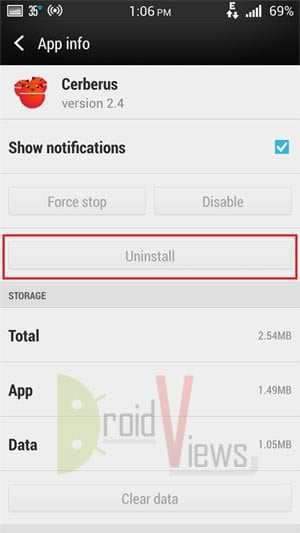
\includegraphics[width=0.8\columnwidth]{figures/DA.png}
%DIFDELCMD < %%%
%DIFDELCMD < \caption{%
{%DIFAUXCMD
\DIFdelFL{An example of an app disabling both the
Force Stop and Uninstall buttons on Android 6.}}
%DIFAUXCMD
%DIFDELCMD < \label{fig:da}
%DIFDELCMD < \end{figure}
%DIFDELCMD < 

%DIFDELCMD < %%%
\DIFdelend Figure~\ref{fig:da} shows an example of an app disabling both the Force Stop and Uninstall buttons on a phone running Android 6. \DIFaddbegin \DIFadd{Table~\ref{tab:add_app_info} shows the list of spyware of apps we chose, their APK version code, and the SHA-1 hash for the corresponding APK we study.
}

\begin{figure}[t]
\centering
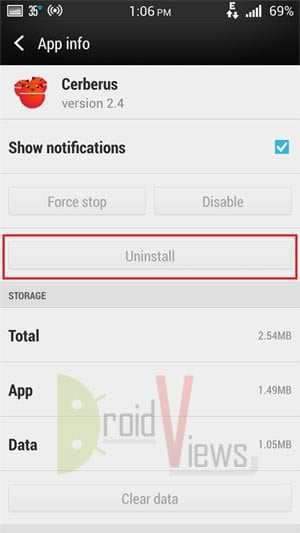
\includegraphics[width=0.8\columnwidth]{figures/DA.pdf}
\caption{\DIFaddFL{An example of an app disabling both the
Force Stop and Uninstall buttons on Android 6.}}
\label{fig:da}
\end{figure}
\DIFaddend 







%%%%%%%%%%%%%%%%%%%%%%%%%%%%%%%%%%%%%%%%%%%%%%%%%%%%%%%%%%%%%%%%%%%%%%%%%%%%%%%%
\end{document}
%%%%%%%%%%%%%%%%%%%%%%%%%%%%%%%%%%%%%%%%%%%%%%%%%%%%%%%%%%%%%%%%%%%%%%%%%%%%%%%%

%%  LocalWords:  endnotes includegraphics fread ptr nobj noindent
%%  LocalWords:  pdflatex acks
